
\documentclass[twocolumn,doublespacing]{aastex631} 
\usepackage{amsmath}
\usepackage{mathtools}
%\usepackage{lineno}
\usepackage{appendix}
\usepackage{dsfont}
\usepackage{listings}
\usepackage{placeins}
\usepackage{booktabs}
\newcommand{\vdag}{(v)^\dagger}
\newcommand\aastex{AAS\TeX}
\newcommand\latex{La\TeX}
\newcommand{\mearth}{M$_\oplus$}
\usepackage{hyperref}

\shorttitle{Tidal Forces on `Oumuamua}
\shortauthors{Taylor et al.}

\graphicspath{{./}{figures/}}


\begin{document}
\title{Assessing Potential Contributions from Outgassing and Tidal Effects on the Evolving Rotational State of 1I/`Oumuamua}

\correspondingauthor{Aster Taylor}
\email{astertaylor@uchicago.edu}
\author[0000-0002-0140-4475]{Aster G. Taylor}
\affiliation{Dept. of Astronomy and Astrophysics, University of Chicago, 5640 S Ellis Ave, Chicago, IL 60637} 

\author[0000-0002-0726-6480]{Darryl Z. Seligman}
\affiliation{Dept. of Astronomy and Carl Sagan Institute, Cornell University, 122 Sciences Drive, Ithaca, NY, 14853, USA}

\author[0000-0003-0647-6176]{Douglas R. MacAyeal}
\affil{Dept. of Geophysical Sciences, University of Chicago, 5734 S Ellis Ave, Chicago, IL 60637}

\author[0000-0001-6952-9349]{Olivier R. Hainaut}
\affiliation{European Southern Observatory, Karl-Schwarzschild-Strasse 2, Garching bei München, D-85748, Germany}

\author[0000-0002-2058-5670]{Karen J. Meech}
\affil{Institute for Astronomy, University of Hawaii, 2680 Woodlawn Drive, Honolulu, HI 96822, USA}

\begin{abstract}

In this paper, we attempt to interpret the photometric light curve of 1I/`Oumuamua, the first interstellar object discovered traversing the inner Solar System. We compare photometric data with synthetic light curves of ellipsoidal bodies for a range of rotational states and observing geometries. While previous work reported an increase in the periodicity of the object during October, we find a $\Delta p\simeq0.21$ hour decrease in the spin period between October and November. We investigate potential contributions to the evolving spin period from both outgassing and tidal effects using a general formalism which may be applied to any elongated object. While sublimation is a stronger effect, tidal deformation could change the moment of inertia and subsequent spin period based on the bulk material properties. We present an open source software which simulates constant-density liquid bodies subject to tidal forces for a range of assumed viscosites and sizes (\texttt{SAMUS}). These numerical simulations, when applied to `Oumuamua, demonstrate that it may have experienced significant tidal deformation in the presence of sublimation. However, synthetic observations which incorporate tidal effects demonstrate that little deformation is necessary to match the composite light curve. We find that a dynamic viscosity of $\mu\geq10^9$ g cm$^{-1}$ s$^{-1}$, corresponding to a 0.1\% change in moment of inertia, best reproduces the photometric data. This allowable viscosity range is compatible with materials such as water ice, bitumen pitch, and the terrestrial mantle. It is feasible that tidal deformation contributed to the shorter timescale spin-down in October, while outgassing induced the secular spin-up. 

\end{abstract}

%\keywords{Interstellar Objects}
\keywords{Interstellar Objects (52); Comets (280); Hydrodynamics (1963)}

\section{Introduction}

In October 2017, the Minor Planet Center announced the discovery of 1I/2017 U1, a small body which was extrasolar in nature \citep{mpec2017}, later named 1I/‘Oumuamua. By the time this object was discovered, it had already passed its perihelion and was quickly departing from the Solar System. 

There was an immediate acquisition of ground- and space-based observations of the rapidly fading object. These observations produced a high-quality composite light curve spanning approximately a month (29.3 days) and a spatial segment of $l\simeq0.13$ au. In total there were 818 observations, reported by \citet{meech2017}, \citet{bolin2017}, \citet{bannister2017}, \citet{drahus2017}, \citet{fraser2018}, \citet{jewitt2017}, \citet{knight2017}, and \citet{belton2018}. These observations were collected in \citet{belton2018}. `Oumuamua was interpreted to be highly elongated, with an aspect ratio estimated to be $>$3:1 \citep{bolin2017,knight2017}, $>$5:1 \citep{bannister2017,fraser2018,jewitt2017}, and up to 10:1 \citep{meech2017}. Frequency analysis of the light curve showed a maximum at a period of $p\simeq4.3$ hours \citep{belton2018}. This was interpreted to be half of the rotational period --- corresponding to a revolution of 180$^\circ$. `Oumuamua's variations in absolute magnitude of $H\simeq22.5\pm1.3$ over its rotation led to the conclusion that it was exhibiting complex, non-principal axis rotation \citep{drahus2017,meech2017,fraser2018}.

This analysis was further refined by \citet{mashchenko2019} who demonstrated via full light curve modeling that a near-symmetric oblate ellipsoid with dimensions of 115:111:19$\sim$6:6:1 meters provided a best fit geometry for the light curve data. This size estimate assumes a geometric albedo of $A=0.1$ and would change with a different albedo, but with appropriately scaled dimensions. While a prolate ellipsoid with dimensions of 342:42:42 meters is also allowable, the torques required to replicate the motion are highly tuned, so the prolate geometry is disfavored. 

Deep imaging revealed a notable lack of cometary activity, classifying `Oumuamua as an asteroidal body and restricting possible dust outputs (upper limits range from $\sim2\cdot10^{-4}$ kg s$^{-1}$ \citep{jewitt2017} to $1.7\cdot10^{-3}$ kg s$^{-1}$ \citep{meech2017}). Additionally, while outbound at 2 au, there was a significant non-detection of the object with the \textit{Spitzer Space Telescope}. This non-detection placed limits on the production of CO and CO$_2$ \citep{trilling2018}. 

Astrometric positional data revealed that the trajectory was inconsistent with pure Keplerian motion \citep{micheli2018}. The addition of a radially outward non-gravitational acceleration of the form $a=4.92\cdot10^{-4}\, (r/1\, {\rm au})^{-2}\, \boldsymbol{\hat{r}}$ cm s$^{-2}$ provides a greatly improved, $30\sigma$ fit to the trajectory.\footnote{An acceleration with a form of $r^{-1}$ is nearly as good of a fit.} \citet{micheli2018} proposed a comet-like outgassing as an explanation for this acceleration, ruling out radiation pressure, the Yarkovsky effect, magnetic forces, and others which would require extreme physical properties.

The restrictions on the coma and micron-scale dust presence in the vicinity are quite stringent. Therefore, theories for the provenance of the object positing cometary outgassing as the source of the acceleration require additional complexity to avoid violating the \textit{Spitzer} or photometric observations.\footnote{Although the original Spitzer estimates had a computational error, see \citet{seligman2021}. Even these revised CO limits, however, are prohibitive to the $1/r^2$ fit.} H$_2$O ice was initially proposed as an outgassing accelerant because it is the most common volatile in Solar System comets \citep{Rickman2010,Ahearn2012,Ootsubo2012,Cochran2015,Biver2016,Bockelee2017} and its presence is not in tension with the \textit{Spitzer} non-detection. However, the relatively high enthalpy of sublimation (51 kJ mol$^{-1}$) of H$_2$O implies that water sublimation would require more energy input than `Oumuamua received from solar radiation \citep{sekanina2019}.

Attempting to unify these constraints, \citet{SL2020} argued that only hypervolatiles could serve as the accelerant for `Oumuamua. They found that only molecular hydrogen (H$_2$), neon, molecular nitrogen (N$_2$), and argon were allowable accelerants for an oblate spheroid --- although CO was also shown to be energetically feasible. Those authors also investigated the feasibility of hydrogen ice as the bulk constituent --- originally hypothesized by \citet{fuglistaler2018solid} --- as it requires the lowest active surface fraction to be explanatory. In this hypothesis, `Oumuamua would have formed in a failed prestellar core in a Giant Molecular Cloud. This model naturally explains the extreme shape (via continuous H$_2$ ablation), the low excess velocity speed, and young age \citep{mamajek2017,Gaidos2017a, Feng2018,Fernandes2018,hallatt2020,Hsieh2021}. However, there are theoretical barriers to the formation of macroscopic bodies composed of solid hydrogen, such as the frigid temperatures required for formation and rapid evaporation in the interstellar medium \citep{hoang2020,phan2021,levine2021,LL2021}. Although the low condensation temperature of molecular hydrogen ($<$10K) poses difficulties for its formation, \citet{LL2021} demonstrated that adiabatic expansion pockets were a plausible formation environment for such an object.

\citet{jackson2021} instead suggested that `Oumuamua was composed of molecular nitrogen (N$_2$) ice, while \citet{desch2021} proposed that impacts on extrasolar Pluto analogues would provide a plausible source for objects like `Oumuamua. However, \citet{levine2021} demonstrated that the necessary mass density for this formation to be plausible is unreasonably high.

\citet{seligman2021} found that a typographical mistake in \citet{trilling2018} led to the reported outgassing limits of CO to be underestimated by two orders of magnitude. When this error was corrected for, those authors showed that a body characterized by a modest covering fraction of CO exhibiting sporadic activity could explain both the acceleration and Spitzer observations. 

However, all outgassing hypotheses fail to explain the lack of a dust coma satisfactorily. \citet{micheli2018} and \citet{seligman2021} argued that the post-perihelion detection of `Oumuamua could explain the lack of dust, since subsurface cometary layers are expected to be enriched with larger dust grains \citep{laufer2005,micheli2018}, and `Oumuamua had likely already lost a fraction of its surface at detection \citep{SLB2019,SL2020,desch2021,jackson2021}. In addition, the interstellar medium would remove small dust grains from the surface of such interstellar objects \citep{stern1987,stern1990} via drag effects, particularly when passing through supernova remnants.

Finally, \citet{micheli2018} considered and rejected radiation pressure as the source of the anomalous acceleration, since this would require `Oumuamua to have bulk densities of $\rho<10^{-5}$ g cm$^{-3}$. However, \citet{bialyloeb2018}, \citet{moro-martin2019}, \citet{flekkoy2019}, \citet{luu2020}, and \citet{sekaninacomet} proposed various geometries and compositions which would allow radiation pressure to produce the non-ballistic trajectory. \citet{bialyloeb2018} explored radiation pressure in the context of a millimeter-thick minor axis geometry implying an artificial origin. However, radio signals from the object were not detected \citep{Enriquez2018,Tingay2018,Harp2019} and there is a $\sim$1\% probability for this geometry to produce the observed brightness variations \citep{Zhou2022}. \citet{sekaninacomet} proposed a disintegrated dwarf comet as an origin. \citet{moro-martin2019}, \citet{flekkoy2019}, and \citet{luu2020} proposed that `Oumuamua could be a fractal, hyper-porous dust aggregate, formed either in a proto-planetary disk \citep{moro-martin2019} or in the inner coma of an Oort-cloud comet \citep{flekkoy2019,luu2020}. Other theories have invoked circumbinary systems \citep{Cuk2017,Jackson2017,Childs2022}, tidal fragmentation \citep{Raymond2018b,zhang2020tidal,Raymond2020}, and/or ejection from post-main sequence stars \citep{Hansen2017,Rafikov2018c,Katz2018}. 

The material composition of `Oumuamua and the source of its anomalous acceleration remain unclear. For recent reviews, see \citet{Jewitt2022ARAA} and \citet{MoroMartin2022}. Until now, shearing effects due to tidal forces have been ignored in the context of an icy cometary body. At perihelion, `Oumuamua passed within $r_H\simeq0.256$ au of the Sun, subjecting it to non-trivial tidal stresses --- although attempts to pre-discover the object here resulted in non-detections \citep{hui2019}. The tidal stresses, combined with the large-magnitude centrifugal force produced by `Oumuamua's high aspect ratio and rapid rotation, produce significant shearing stress on the body. By modeling `Oumuamua as a fluid body,\footnote{Semi-crystalline solids such as ices are commonly modeled as fluids, since they deform continuously under pressure.} we investigate the effects of these shearing forces to provide constraints on the size and bulk dynamic viscosity of `Oumuamua. The latter could provide a constraint on the possible material composition of `Oumuamua.

Unfortunately, these constraints are weakened by the difficulty of measuring the viscosity of proposed materials. While water ice has a known dynamic viscosity of $10^{13}$ g cm$^{-1}$ s$^{-1}$ \citep{fowler1997}, exotic solids such as CO, H$_2$, and N$_2$ ice are far more difficult to measure. \citet{vilelladeschamps2017} analyzed the dynamics of N$_2$ ice glaciers in the Sputnik Planitia of Pluto, and found that the observed polygonal structure is consistent with viscosities of $10^{15}$--$10^{17}$ g cm$^{-1}$ s$^{-1}$, although these values are not well-constrained and are highly uncertain. Due to experimental barriers, however, no measurements are available for the viscosity of H$_2$ or CO ice. In addition, the structural composition of and material mixing within the body further complicates the viscosity measurements. Despite these practical difficulties, constraining the material properties provides a new methodology to test proposed structures and compositions for `Oumuamua, future interlopers of this type, and Solar System minor bodies. 

\citet{flekkoy2019} considered the effects of tidal forces in the context of a dust aggregate and demonstrated a surprising stability against tidal stresses. On the other hand, outgassing of the scale necessary to provide the acceleration would have been significantly stronger than tidal forces on the small object. The tidal acceleration is $a_{\rm tidal}\simeq GM_\Sun (1/(r_H-x)^2-1/r_H^2)$, where $M_\Sun$ is the Solar mass, $r_H$ is the heliocentric distance, and $D$ is the maximum size of the object. At 1 au, with an object size of $D\simeq100$ m, the tidal acceleration is $a\simeq10^{-9}$ cm s$^{-2}$, approximately 5 orders of magnitude smaller than the observed non-gravitational acceleration. However, tidal forces may have been comparable to outgassing forces when `Oumuamua approached perihelion at $r_H\simeq0.256$au. Moreover, depending on the material properties, tidal forces may have distorted the shape in the presence of outgassing. This distortion may have induced observational signatures in the rotational state and light curve.

This paper is organized as follows: In \S \ref{sec:lightcurvefits}, we identify a decrease in the spin period of `Oumuamua between October and November. We use synthetic light curves (\S\ref{sec:simplemodel}-\ref{subsec:phaseaspectanalysis}) to optimize model parameters to the photometric data in \S\ref{subsec:gettingaxis}. In order to interpret this change in rotational period, we quantify tidal and outgassing torques on elongated small bodies via an idealized 2-dimensional model in \S \ref{sec:bigana}. In \S \ref{sec:numerics}, we present a publicly available open-source code which simulates the response of cometary bodies with arbitrary geometries, bulk material properties, and trajectories to tidal and rotational stress forces. In \S \ref{sec:oumuamuasim}, we present simulations of the deformation of `Oumuamua under tidal stresses throughout its trajectory. In \S \ref{sec:lightcurvesim}, we use these simulations to produce synthetic light curves for `Oumuamua under the action of tidal deformation. In \S \ref{sec:discussion}, we conclude and discuss future research prospects. 

\section{Light Curve Models}\label{sec:lightcurvefits}

In this section, we generate synthetic light curves of `Oumuamua for a range of simplifying assumptions. To validate our methodology, we adopt idealized rotational states and orbital geometries in \S\ref{sec:simplemodel}. We then include complex rotation in \S\ref{subsec:arblightmodel}, and varying phase angles and distances in \S\ref{subsec:evolvinglightmodel}. We fit the photometric brightness variations to obtain optimal parameters for single-axis rotation in \S\ref{subsec:gettingaxis}. Finally, we report a spin-up in `Oumuamua's rotation period between October and November, and resolve tension with the October spin-down identified by \citet{flekkoy2019} in \S\ref{sec:flekkoyana}.

\begin{figure}
\centering
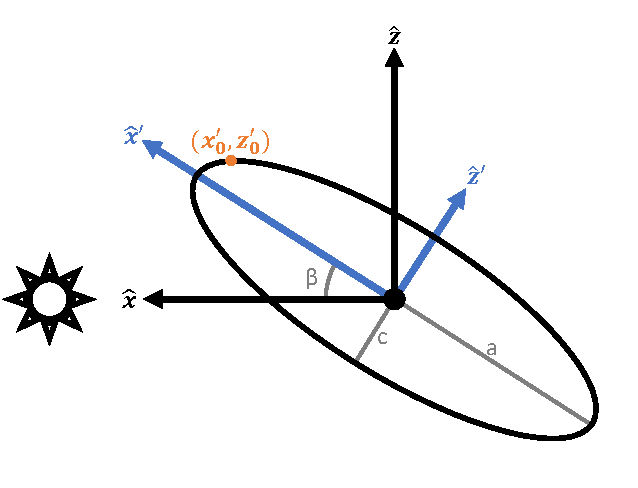
\includegraphics[width=\linewidth,angle=0]{cross_section_ellipse.pdf}
\caption{Diagram of the cross-sectional ellipse. Unprimed coordinates are fixed in the reference frame of the Solar System, while primed coordinates are fixed in the reference frame of the object. The angle $\beta$ defines the rotation state of the body with respect to the Sun. }
\label{fig:ell-cross-section}
\end{figure}

\subsection{Fixed-Position and Fixed-Axis Rotation}\label{sec:simplemodel}

In this subsection, we produce synthetic photometric time series of `Oumuamua assuming single-axis rotation, a simplified viewing geometry, and no modulation from phase angle. We position the Sun, the Earth, and `Oumuamua along the x-axis in conjunction, roughly representative of the astrometric orbital arrangement when `Oumuamua was discovered. The non-rotating unprimed (x, y, z) axes move with `Oumuamua along its trajectory, while the primed coordinate axes (x', y', z') align with the principal axes and co-rotate with the body. We orient the body such that its semi-major principal axes are a:b:c$\sim$6:6:1 \citep{mashchenko2019}, and we assume that `Oumuamua rotates solely about the y-axis. 

We derive the projected area of an ellipsoid with an arbitrary rotation angle (with respect to the x-axis) $\beta$. It is known that any cross-section of an ellipsoid is an ellipse, although possibly with different aspect ratio and orientation. With rotation about the y-axis, the principal axes of the ellipse are along the Cartesian axes, and we solve for the lengths of these 2-dimensional principal axes. The semi-major axis in the y-direction is $b$, and so we now solve for the semi-major axis in the x-z plane which is orthogonal to the rotation axis. In this plane, the cross-section has an aspect ratio of 6:1, with $a=6$ in the x'-direction and $c=1$ in the z'-direction (Figure \ref{fig:ell-cross-section}). The observation vector, defined to be parallel to $\boldsymbol{\hat{x}}$, is rotated about the y-axis such that the rotated axis is $\cos\beta\,\boldsymbol{\hat{x}'}+\sin\beta\,\boldsymbol{\hat{z}'}$, in the primed frame. We then find the location of the points $(x'_0,z'_0)$ where the tangent to the ellipse is parallel to the observation vector, whose projection along the z-axis is this semi-major axis.

The cross-sectional ellipse is defined by the function $f_\text{2d}(x',z')$, where 
\begin{equation}\label{eq:ellipsesimple}
	f_\text{2d}(x',z')=\frac{x'^2}{a^2}+\frac{z'^2}{c^2}-1.
\end{equation}
The tangent $\partial z'/\partial x'$ is the derivative with respect to x of Equation \ref{eq:ellipsesimple}, given by
\begin{equation}
	\frac{\partial z'}{\partial x'}(x)=\mp \frac{c x'}{a^2\sqrt{1-x'^2/a^2}}\,.
\end{equation}
The $\mp$ reflects the degeneracy of the ellipse along slices in the x' axis. The slope of the observation vector in the x'-z' plane is simply $\tan(\beta)$, so by setting $\partial z'/\partial x'=\tan(\beta)$, and simplifying, we obtain 
\begin{equation}\label{eq:csfinalx}
    x'_0=\pm\frac{a^2\tan\beta}{\sqrt{c^2+a^2\tan^2(\beta)}}\,.
\end{equation}
Now by substituting Equation \ref{eq:csfinalx} into $z'=\pm c\sqrt{1-x'^2/a^2}$ (derived from Equation \ref{eq:ellipsesimple}), the points $(x'_0,z'_0)$ are given by
\begin{equation}\label{eq:x0z0}
    (x'_0,z'_0)=(\pm\frac{a^2\tan\beta}{\sqrt{c^2+a^2\tan^2(\beta)}},\mp \frac{c^2}{\sqrt{c^2+a^2\tan^2(\beta)}}).
\end{equation}

The distance between these points and the observation line which passes through the origin is the second semi-major axis of the projected ellipse. For a point $(x'_0,\ z'_0)$, the distance is the projection onto the z-axis, so $d=|\sin\beta\, x'_0+\cos\beta\, z'_0|$. Substituting Equation \ref{eq:x0z0}, the distance is
\begin{equation}
\begin{aligned}
	d=\frac{|a^2\sin\beta\tan\beta+c^2\cos\beta|}{\sqrt{c^2+a^2\tan^2(\beta)}}\,.
\end{aligned}
\end{equation}
Since the area of the ellipse is $\pi b d$, the brightness $L_\text{fix}$ (with simplification) is given by
\begin{equation}\label{eq:fixedlightcurve}
	L_\text{fix}=\pi b\sqrt{(a\sin\beta)^2+(c\cos\beta)^2}. 
\end{equation}
We verified (not shown) that this simple analytic model roughly reproduces the photometric data given in \citet{belton2018}.

\subsection{Fixed-Position and Arbitrary Single-Axis Rotation}\label{subsec:arblightmodel}

In this subsection, we add an arbitrary rotation axis with fixed orbital positioning and produce a numerical light curve model. We again assume that the ellipsoid has principal semi-major axes $a,b,c$ along the x, y, and z axes respectively. The instantaneous rotational state is defined by the matrix $\boldsymbol{R}^{-1}$, which maps from the unprimed, fixed frame to the primed body frame. As before, the observation direction is defined to be along $\boldsymbol{\hat{x}}$. 

We first generate a collection of points in the body frame which satisfy the ellipsoid function $f_\text{3d}(x',y',z')$ defined as
\begin{equation}
  f_\text{3d}(x',y',z')= \frac{x'^2}{a^2}+\frac{y'^2}{b^2}+\frac{z'^2}{c^2}-1=0\,.
\end{equation}
We then project all of these points into the plane orthogonal to the observation direction, thereby removing a dimension. For a point vector $\boldsymbol{r}$ and observation direction $\boldsymbol{\hat{e}}_\Earth$, the projection into this plane is $\boldsymbol{r}_{\|}=\boldsymbol{r}-(\boldsymbol{r}\cdot\boldsymbol{\hat{e}}_\Earth)\boldsymbol{\hat{e}}_\Earth$, where `$\cdot$' represents a vector dot product. We then rotate these points to the y-z plane by taking $\boldsymbol{R}*\boldsymbol{r}_{\|}$, where `$*$' represents matrix multiplication. 

With these 2-dimensional points, we use the SciPy function \texttt{scipy.spatial.ConvexHull} \citep{scipy} to extract all points defining the convex hull (the smallest convex set which contains all of the projected points). Here, the total surface area of the hull is the projected surface area of the rotated ellipsoid. The brightness again scales with the projected area, so this area is defined to be the reflected brightness $L_\text{arb}$.

This numerical approximation is only precise for a large number of points --- as the number of sampled points $N\rightarrow\infty$, the error of this approximation $E\rightarrow0$. We therefore compare this model to the analytic model given in \S\ref{sec:simplemodel} for $N\simeq$ 4,000, $N\simeq$ 15,000 and $N\simeq$ 60,000 points versus the analytical model, by setting the rotation axis and principal axes to be equal. The fractional errors $E_{\rm frac}$ for these $N$-values, which are defined as 
\begin{equation}\label{eq:frac_err}
  E_\text{frac}\equiv\,\bigg(\,\frac{|L_\text{fix}-L_\text{arb}|}{L_\text{fix}}\,\bigg)\,,
\end{equation} 
are plotted in Figure \ref{fig:numer_light_comparison}. An order of magnitude increase in the number of points reduces the error by nearly an order of magnitude, demonstrating numerical convergence.

\begin{figure}
\centering
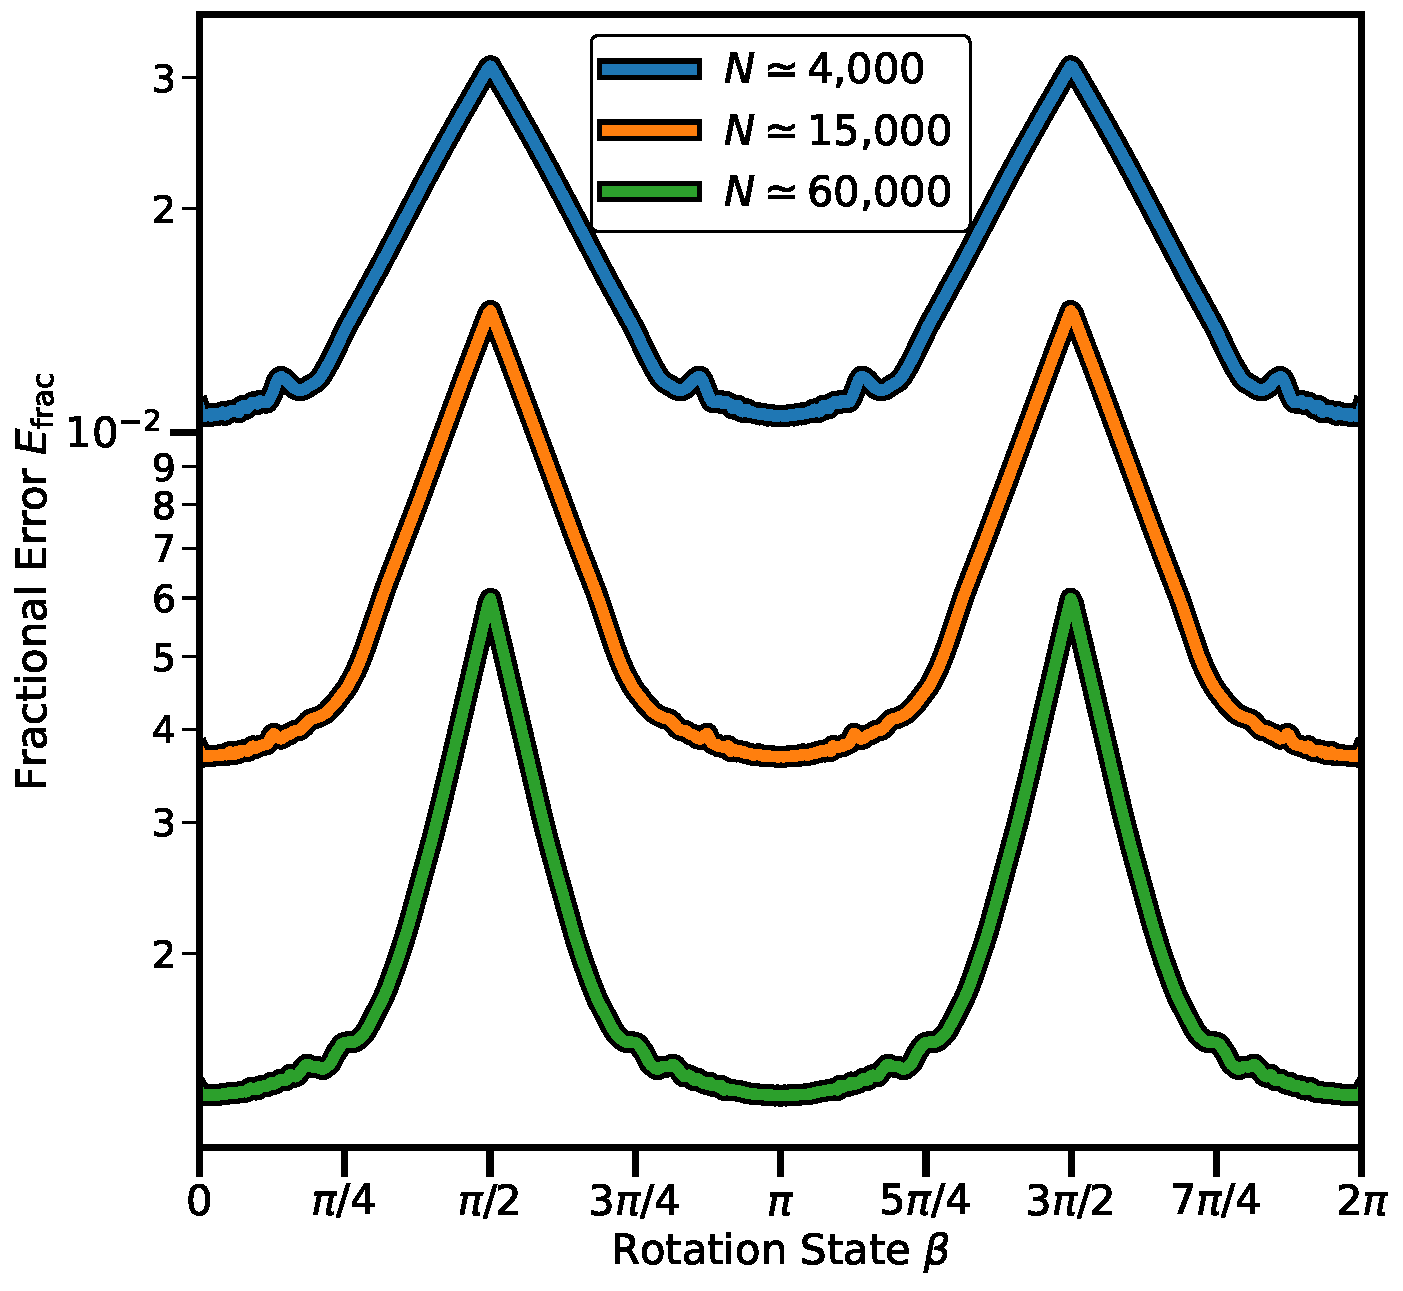
\includegraphics[width=\linewidth,angle=0]{num_lightcurve_comp.pdf}
\caption{Fractional error (Equation \ref{eq:frac_err}) of the fixed- and arbitrary-axis light curve models. }
\label{fig:numer_light_comparison}
\end{figure}

\subsection{Evolving-Position and Single-Axis Rotation}\label{subsec:evolvinglightmodel}

In this subsection, we include the motion of the Earth and `Oumuamua in our model. We use Equation 10 from \citet{muinonen2015}, which we refer to as `ML15' for the remainder of this paper. We assume that `Oumuamua has a diffuse Lommel-Seeliger scattering surface, which represents a closely-packed particulate medium with weak multiple scattering. Integrating the Lommel-Seeliger scattering fucntion over the exposed-and-visible surface gives an expression for the brightness at any orientation.

We assume a single-scattering albedo $A$ and an isometric single-scattering phase function $P(\alpha)=1$. This incorporates modulation based on the body orientation, but assumes no additional modulation from the scattering function. We define the phase angle $\alpha$ as the interior Sun-object-Earth angle, and note that $\cos\alpha=\boldsymbol{\hat{e}}_{\Sun}\cdot\boldsymbol{\hat{e}}_{\Earth}$, where $\boldsymbol{\hat{e}}_{\Sun}$ and $\boldsymbol{\hat{e}}_\Earth$ are unit vectors in the direction of the Sun and Earth respectively. We also define the matrix $\boldsymbol{C}$ as
\begin{equation}
    \boldsymbol{C}\equiv\begin{pmatrix}
    \frac{1}{a^2} & 0 & 0\\
    0 & \frac{1}{b^2} & 0\\
    0 & 0 & \frac{1}{c^2}
    \end{pmatrix}\,,
\end{equation}
and the parameters $T_{\Sun}$ and $T_\Earth$ to be
\begin{equation}
    \begin{aligned}
        T_{\Sun}\equiv&\sqrt{\boldsymbol{\hat{e}}_{\Sun}^TC\boldsymbol{\hat{e}}_\Sun}\\
        T_\Earth\equiv&\sqrt{\boldsymbol{\hat{e}}_\Earth^TC\boldsymbol{\hat{e}}_{\Earth}}\,.
    \end{aligned}
\end{equation}
We further define the parameter $T$ as
\begin{equation}
    T\equiv\sqrt{T_{\Sun}^2+T_\Earth^2+2T_{\Sun}T_\Earth\cos\alpha'}\,,
\end{equation}
the angle $\alpha'$ as 
\begin{equation}
\begin{aligned}
    \cos\alpha'=&\frac{\boldsymbol{\hat{e}}_{\Sun}^TC\boldsymbol{\hat{e}}_\Earth}{T_{\Sun}T_\Earth}\\
    \sin\alpha'=&\sqrt{1-\cos^2\alpha'}\,,
\end{aligned}
\end{equation}
and the angle $\lambda'$ as 
\begin{equation}
\begin{aligned}
    \cos\lambda'=&\frac{T_\Sun+T_\Earth\cos\alpha'}{T}\\
    \sin\lambda'=&\frac{T_\Sun\sin\alpha'}{T}\,.
\end{aligned}
\end{equation}
Then the disk-integrated brightness $L_{\rm ML15}$ is 
\begin{equation}
\begin{aligned}
    L_{{\rm ML15}}(\alpha)=&\frac{1}{8}\pi F_0AP(\alpha)abc\frac{T_\Sun T_\Earth}{T}\\
    &\bigg(\cos(\lambda'-\alpha')+\cos\lambda'+\sin\lambda'\sin(\lambda'-\alpha')\\
    &\ln{\big[\cot(\frac{1}{2}\lambda')\cot(\frac{1}{2}(\alpha'-\lambda'))\big]}\bigg),
\end{aligned}
\end{equation}
where $\pi F_0$ is the incident flux density. The absolute magnitude is given by
\begin{equation}\label{eq:MLmodel}
\begin{aligned}
        H=\Delta V-&2.5\log\bigg(abc\frac{T_\Sun T_\Earth}{T}\\
        &\big(\cos(\lambda'-\alpha')+\cos\lambda'+\sin\lambda'\sin(\lambda'-\alpha')\\
        &\ln{\big[\cot(\frac{1}{2}\lambda')\cot(\frac{1}{2}(\alpha'-\lambda'))\big]}\big)\bigg),
\end{aligned}
\end{equation}
where $\Delta V$ is a constant to absorb the flux and magnitude conversion \citep{mashchenko2019}.

\begin{figure}
    \centering
    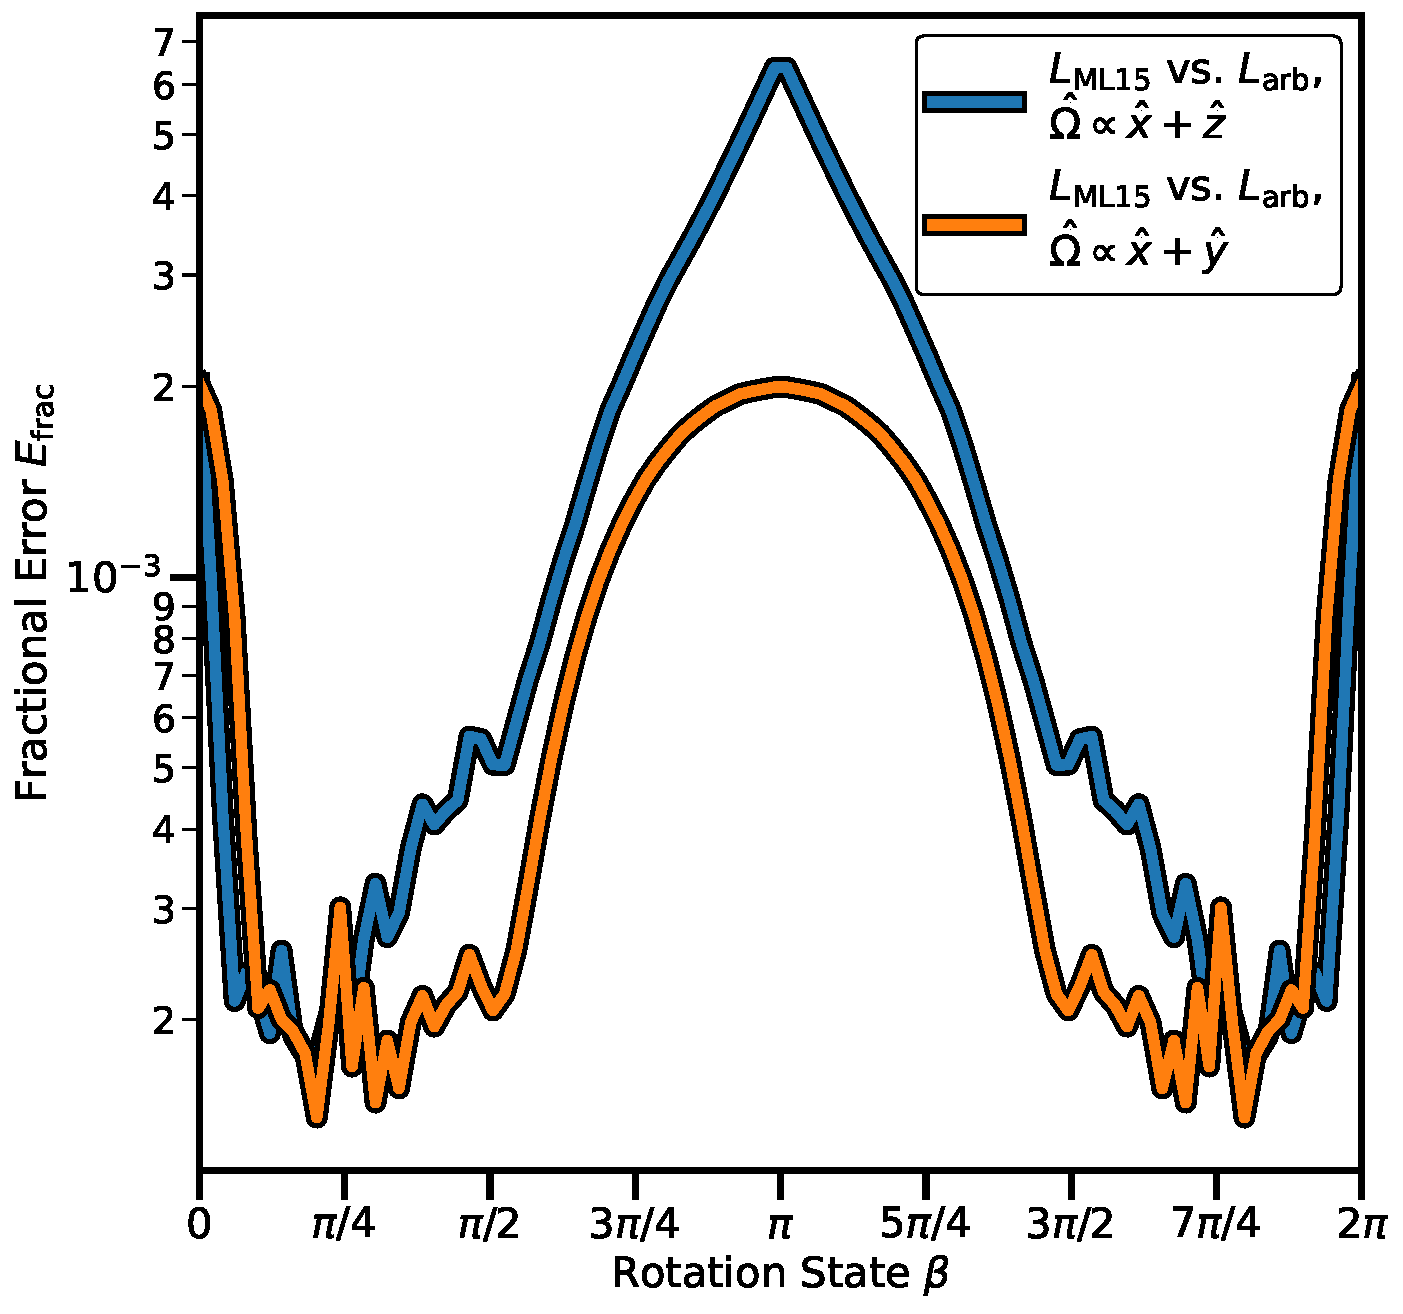
\includegraphics[width=\linewidth,angle=0]{ml_comp.pdf}
    \caption{Fractional error of the ML15 (Equation \ref{eq:MLmodel}) and arbitrary-axis models. Blue and orange curves indicate this comparison for two choices of rotation axes.}
    \label{fig:ml_comparison}
\end{figure}

The fractional error comparing $L_{{\rm ML15}}$ and $L_\text{arb}$ is plotted in Figure \ref{fig:ml_comparison}, with the fractional error defined as $E_\text{frac}\equiv|L_\text{arb}-L_\text{ML15}|/L_\text{arb}$, as in Equation \ref{eq:frac_err}. We show the comparison for rotation axes of $\boldsymbol{\hat{\Omega}}=\boldsymbol{\hat{x}}/\sqrt{2}+\boldsymbol{\hat{z}}/\sqrt{2}$ and $\boldsymbol{\hat{\Omega}}=\boldsymbol{\hat{x}}/\sqrt{2}+\boldsymbol{\hat{y}}/\sqrt{2}$, which were chosen as simple rotational states which produce non-trivial light curves.

The error is comparable to that shown in Figure \ref{fig:numer_light_comparison} for the numerical model, and at machine precision for the fixed-axis model (not shown). We shall use the ML15 evolving-axis model for the remainder of this paper, due to its accuracy and speed.

\begin{figure}
\centering
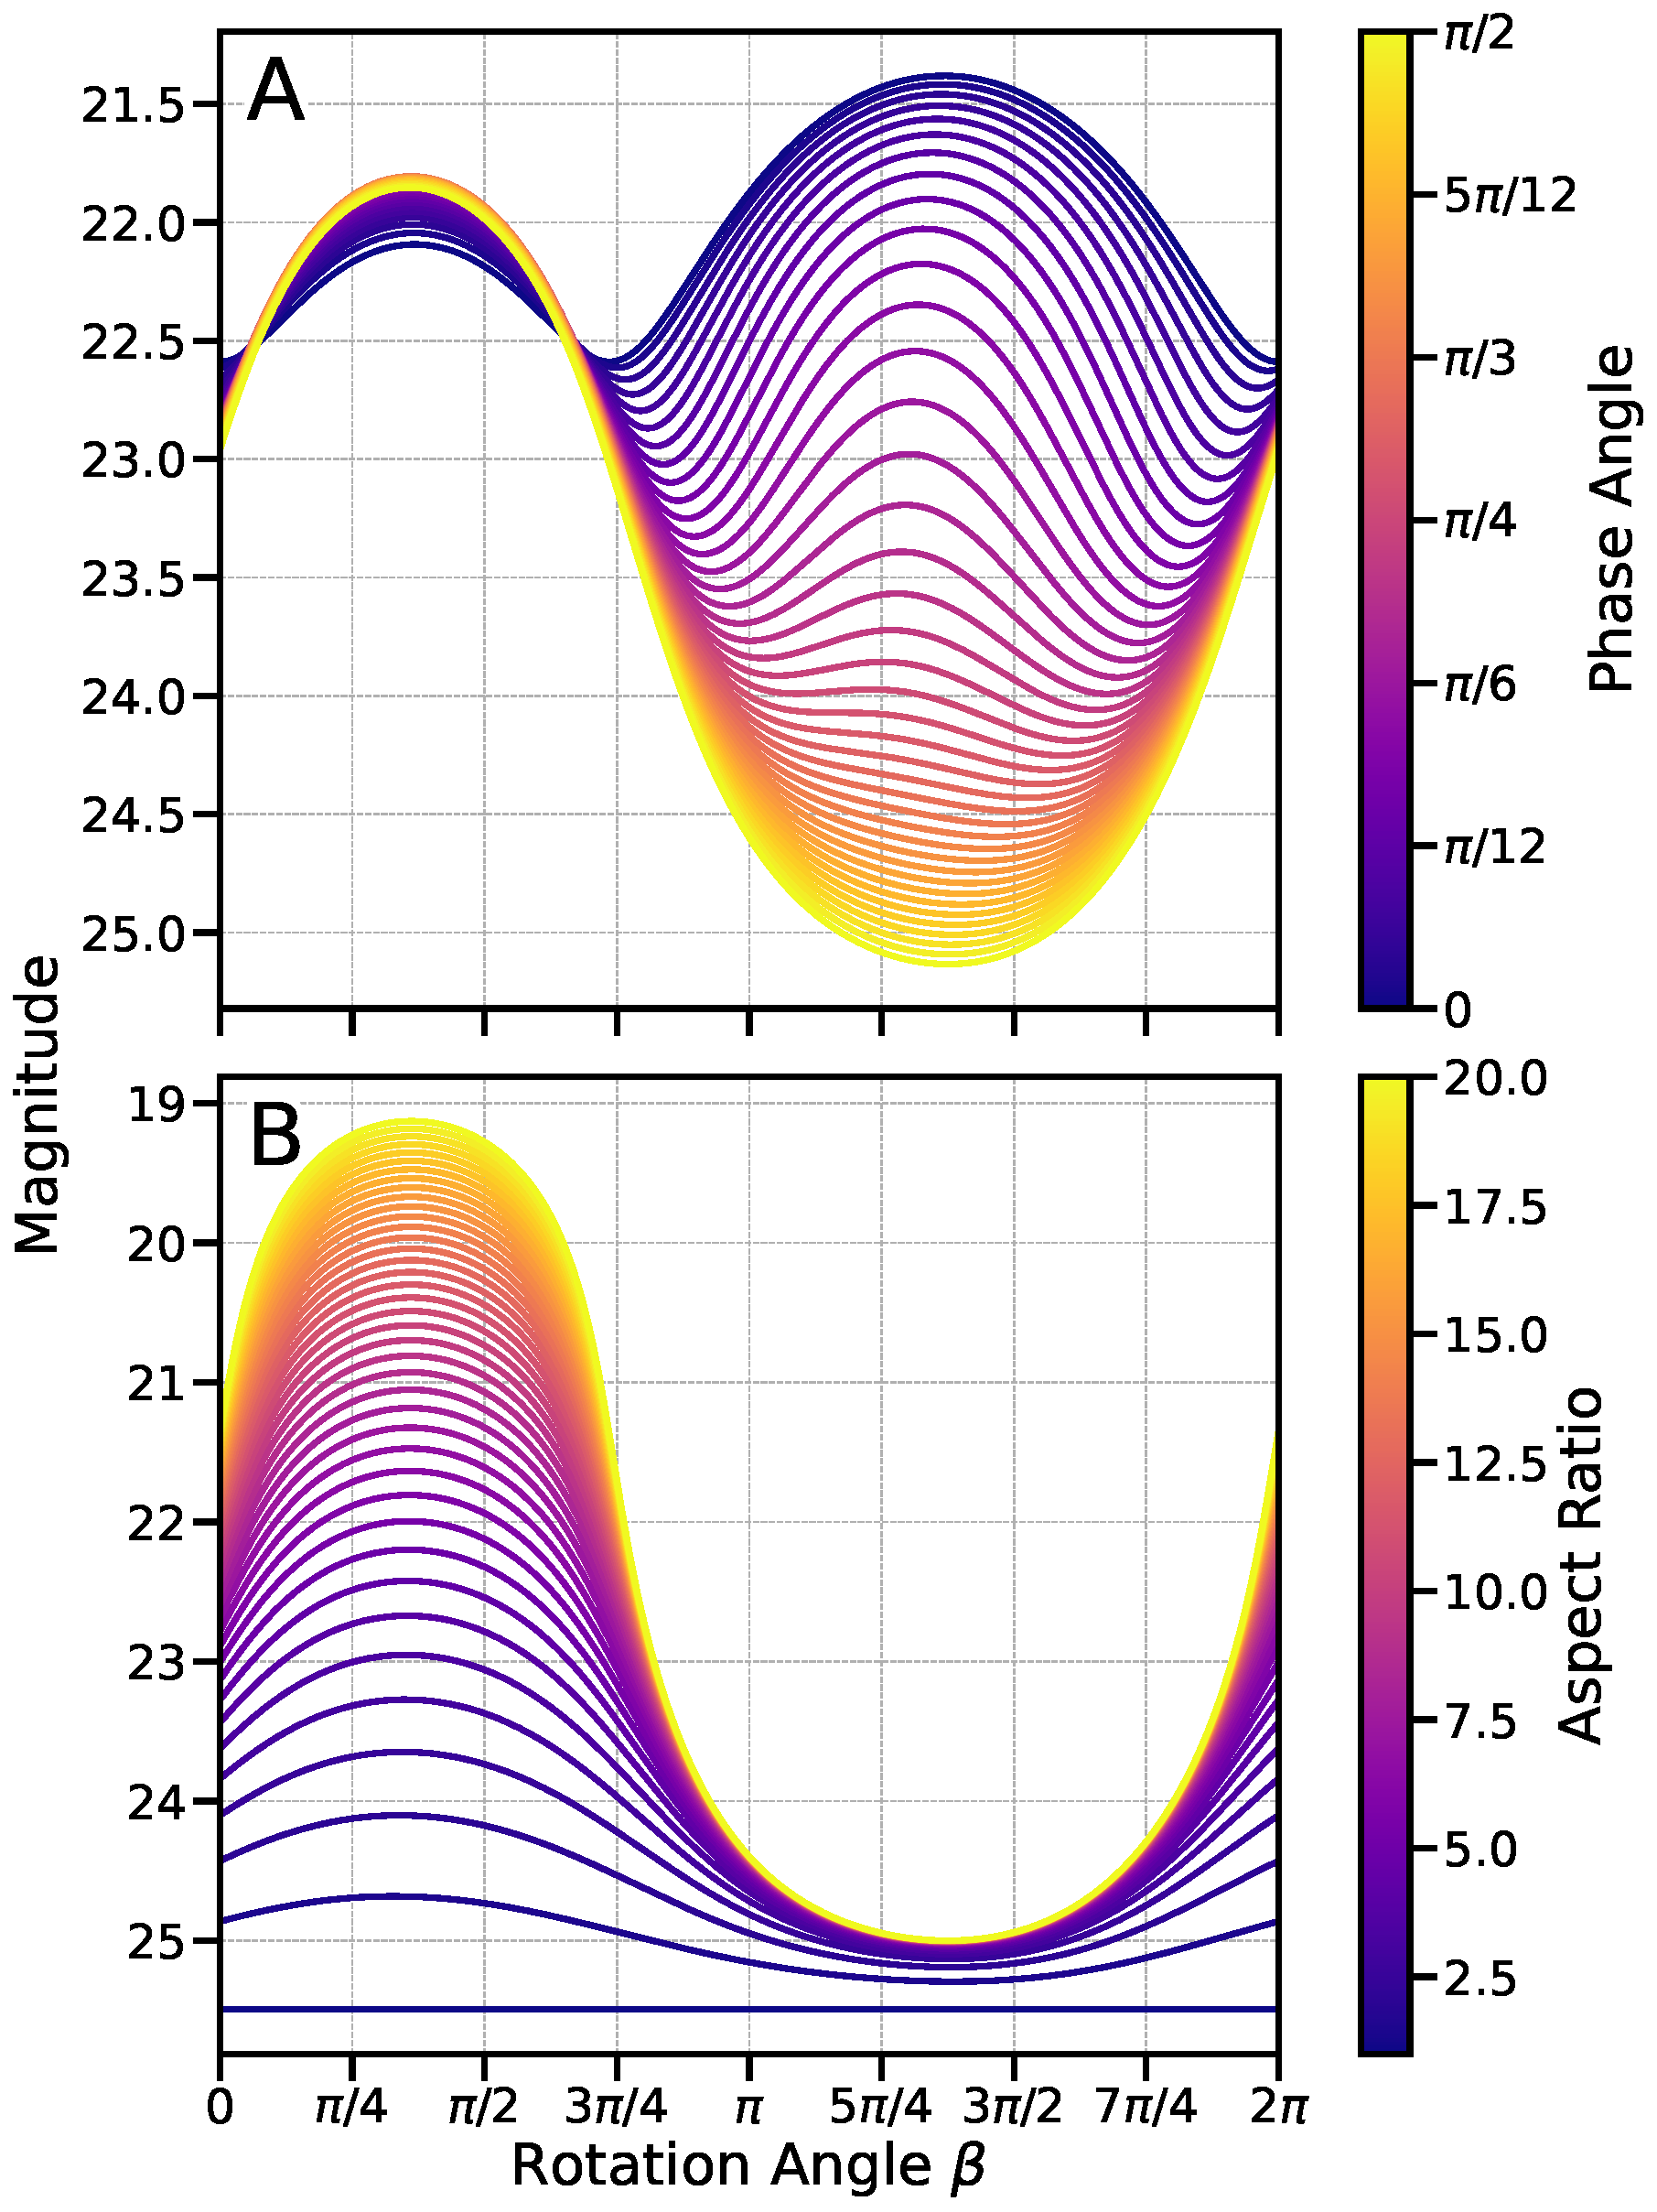
\includegraphics[width=\linewidth,angle=0]{ML15_dependence_effects.pdf}
\caption{Synthetic light curves of a body rotating with an arbitrary period for a range of phase angle (A) and aspect ratio (B). }
\label{fig:phaseeffects}
\end{figure}

\subsection{Phase Angle and Aspect Ratio Dependence}\label{subsec:phaseaspectanalysis}

In this subsection, we investigate the dependence of the ML15 model on phase angle and aspect ratio. We compute synthetic light curves for a single (arbitrary) period with varying phase angle and aspect ratio, and set the parameters ($\theta$, $\phi$, $\psi$, $\beta_0$, and $\Delta V$) to the optimized values given in \S \ref{subsec:gettingaxis}. However, we verified that the phase angle-- and aspect ratio-- dependent behavior of the light curve does not sensitively depend on the other parameters. This analysis both validates the ML15 model and explains components of the synthetic light curves in Figure \ref{fig:optimalaxiscurvesimdata}. 

We present 40 synthetic light curves with phase angles ($\alpha$) uniformly distributed in [$0$,$\pi/2$) and with an aspect ratio of 6:6:1 in Figure \ref{fig:phaseeffects}A. For low phase angle, there are two distinct peaks at $\beta=\pi/2$ and $\beta=3\pi/2$, caused by the half-period cycles of illumination from the larger and smaller cross-sections. As $\alpha\rightarrow\pi/2$, the light curve becomes approximately sinusoidal, as at $\alpha=\pi/2$ only a single face of the body is observable, with brightness variation due to changing exposure. 

We also show 40 synthetic light curves for aspect ratios ranging from 1 to 20 and with $\alpha=\pi/2$ in Figure \ref{fig:phaseeffects}B. Here, the magnitude variation scales with increasing aspect ratio and is zero for a sphere. This effect is simply due to the increasing cross-sectional area contrast for larger aspect ratios. 

\subsection{Obtaining an Optimal Rotation Axis}\label{subsec:gettingaxis}

In this subsection, we use the ML15 model to find an optimal rotational axis for `Oumuamua under the assumption of single axis rotation by fitting a synthetic light curve generated with Equation \ref{eq:MLmodel} to the October photometric data. These data were corrected for light travel time, helio- and geo-centric distance, Solar magnitude, and filter color \citep{belton2018}, and the phase angle data are taken from JPL's Horizons database (\url{https://ssd.jpl.nasa.gov/horizons.cgi}). 

We use the SciPy package's \texttt{scipy.optimize.curve\_fit} for the optimization, which uses a non-linear least squares algorithm to minimize $\chi^2$, where
\begin{equation}
\begin{aligned}
    \chi^2\equiv&\sum_i\left(\frac{(y_i-\mu_i)^2}{\sigma_{y_i}^2}\right)\,.
\end{aligned}
\end{equation}
Here, $y_i$ and $\sigma_{y_i}$ denote photometric measurements and associated errors, while $\mu_i$ denotes corresponding synthetic values. The optimized parameters define the rotation axis and the Earth-pointing axis. 

The Sun-pointing direction $\boldsymbol{\hat{e}}_\Sun$ is along the $\boldsymbol{\hat{x}}$ direction. For a fixed phase angle $\alpha$, the direction of the observer $\boldsymbol{\hat{e}}_\Earth$ is therefore constrained to a cone centered on the x-axis such that $\boldsymbol{\hat{e}}_\Sun\cdot\boldsymbol{\hat{e}}_\Earth=\boldsymbol{\hat{x}}\cdot\boldsymbol{\hat{e}}_\Earth=\cos\alpha$. We then define a new variable $\theta$ such that the direction of the observation is $\boldsymbol{\hat{e}}_\Earth=\cos\alpha\,\boldsymbol{\hat{x}}+\sin\alpha\cos\theta\,\boldsymbol{\hat{y}}+\sin\alpha\sin\theta\,\boldsymbol{\hat{z}}$, with $\theta=0$ if $\boldsymbol{\hat{e}}_\Earth$ lies in the x-y plane.

\begin{figure*}
\centering
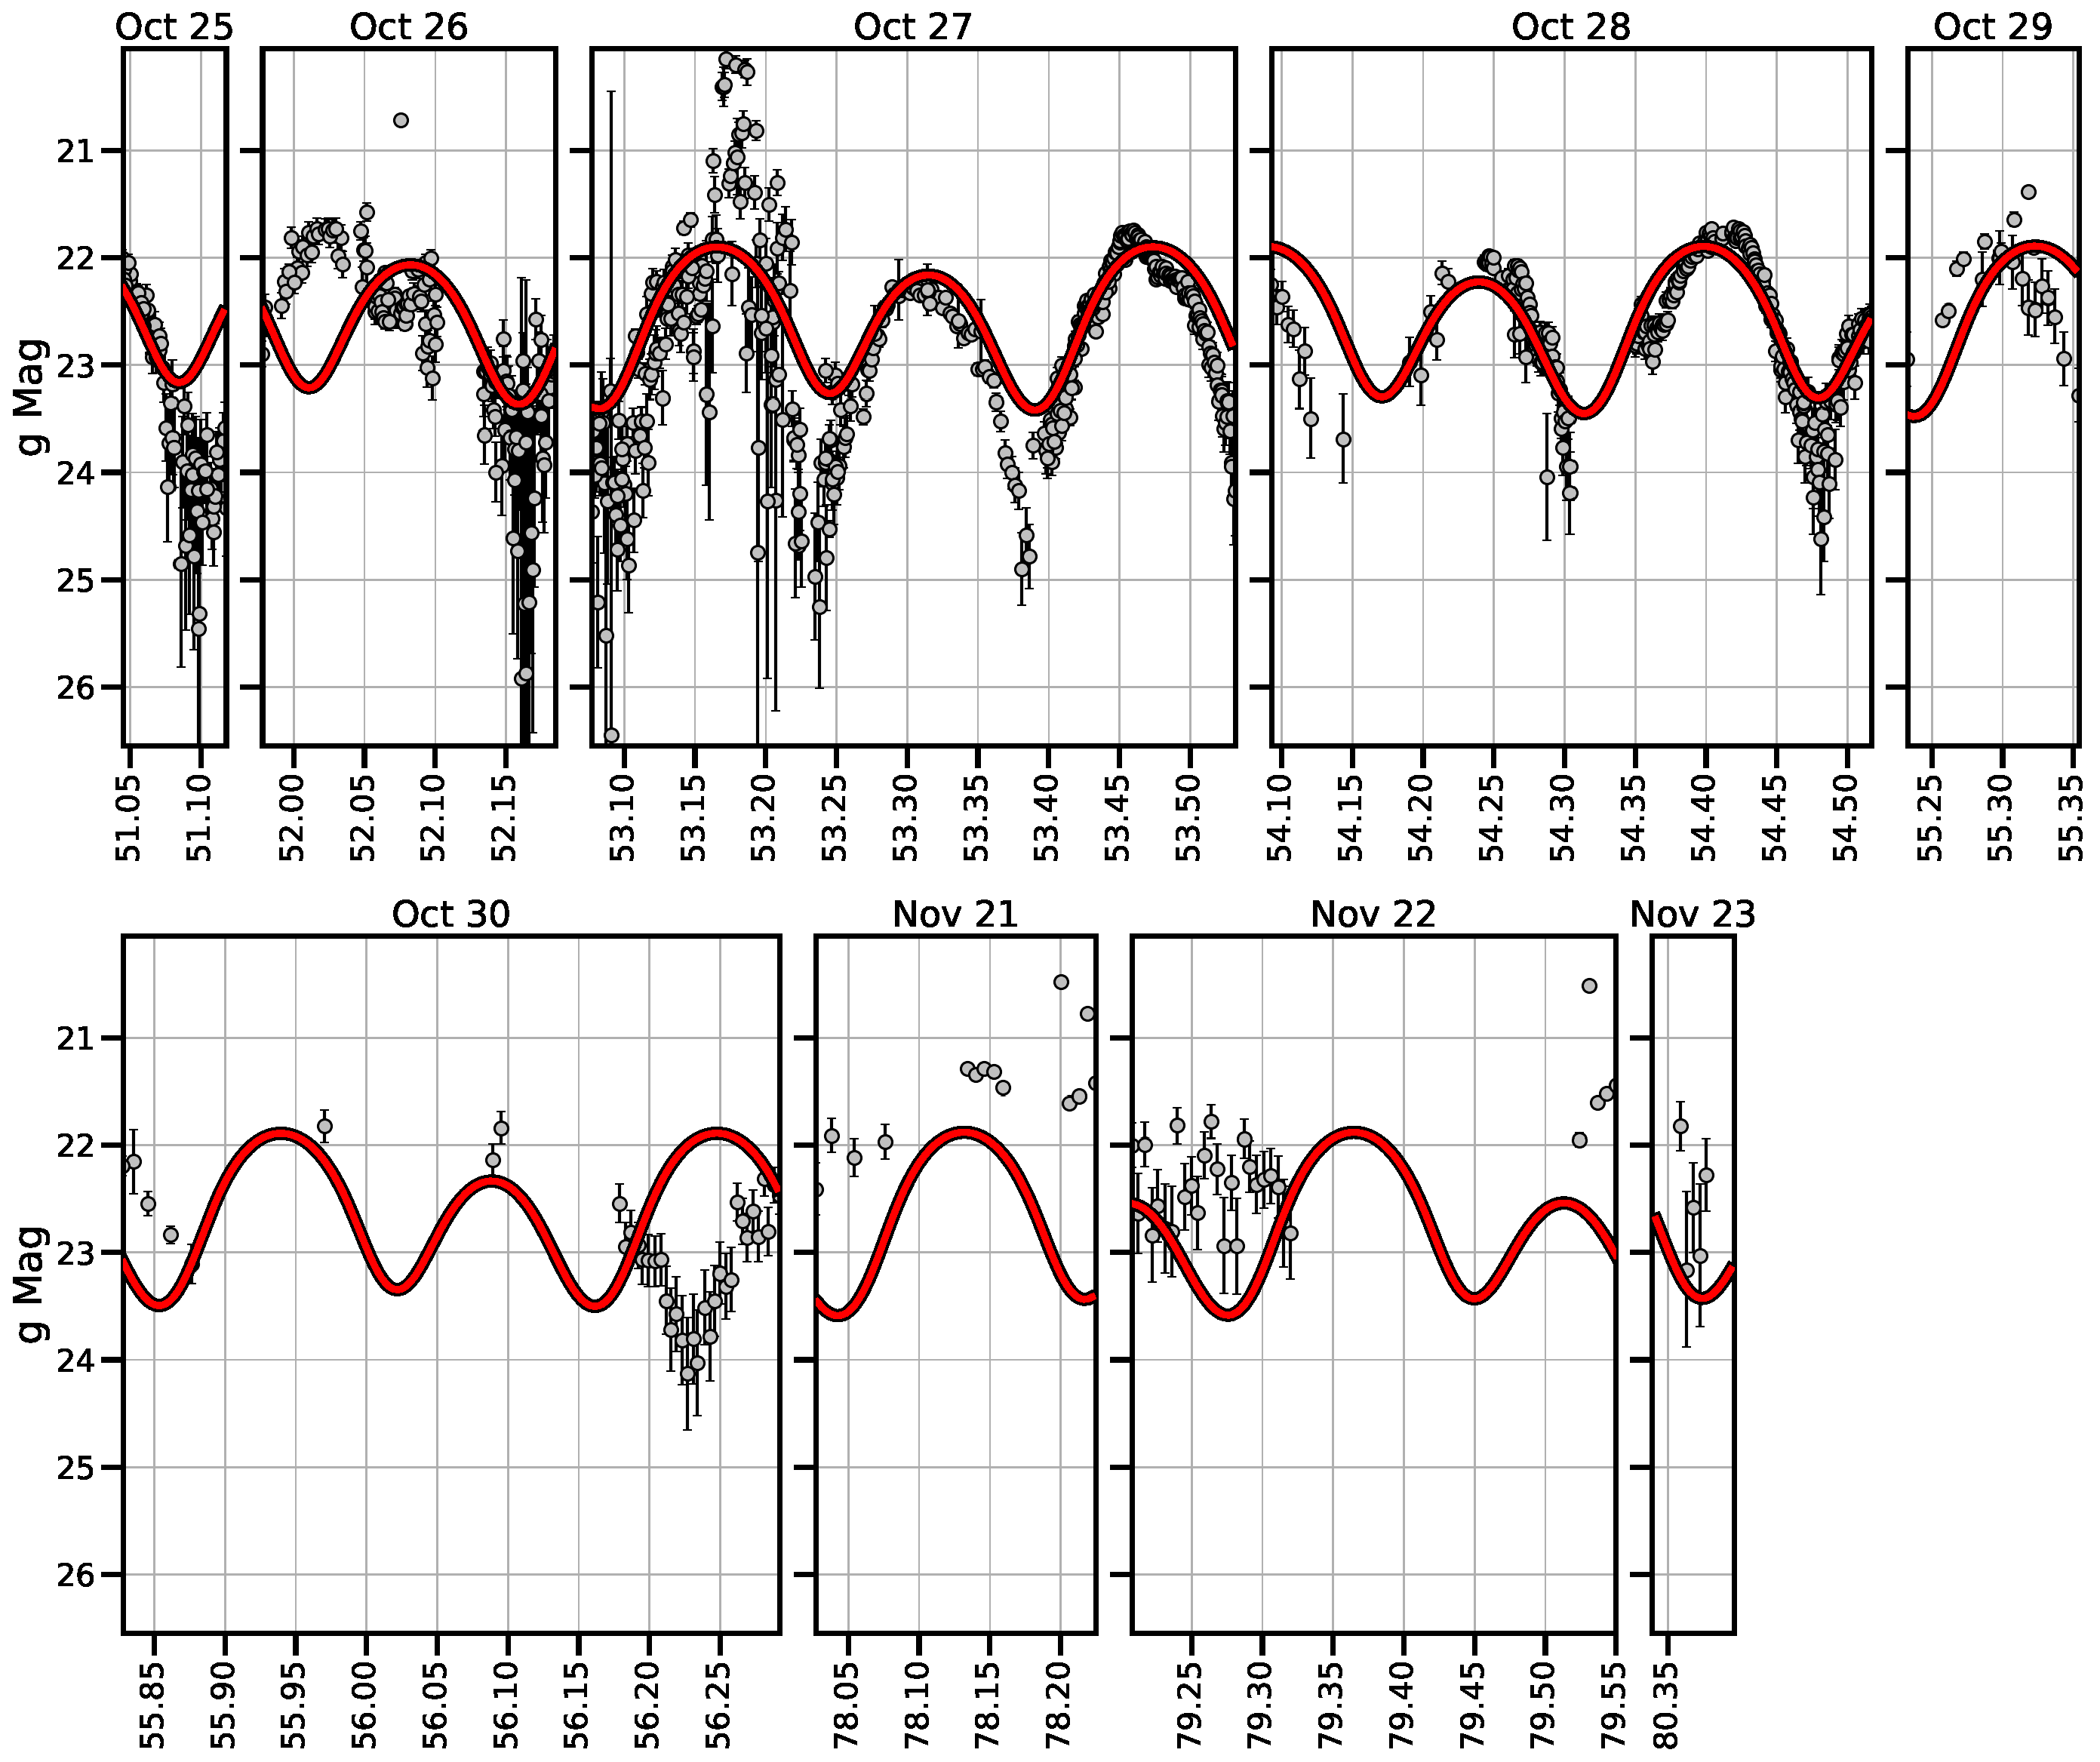
\includegraphics[width=\textwidth,angle=0]{evolving_axis_lightcurve.pdf}
\caption{Synthetic light curve using the ML15 model (red line) alongside photometric observations of `Oumuamua (grey points). The period, initial rotation state, and average magnitude are optimized for the first 6 nights. }
\label{fig:evolvinglightcurve}
\end{figure*}

We additionally parameterize the rotation axis $\boldsymbol{\hat{\Omega}}$ by spherical coordinates about the x-axis. We use a polar angle $\phi$ such that $\boldsymbol{\hat{\Omega}}\cdot\boldsymbol{\hat{x}}=\cos\phi$ and an azimuthal angle $\psi$ measured from the y-axis and restricted to the y-z plane. With these definitions, $\boldsymbol{\hat{\Omega}}=\cos\phi\,\boldsymbol{\hat{x}}+\sin\phi\cos\psi\,\boldsymbol{\hat{y}}+\sin\phi\sin\psi\,\boldsymbol{\hat{z}}$. We restrict the optimization to $\theta\in[0,2\pi)$, $\phi\in[0,\pi/2]$, and $\psi\in[0,2\pi)$ to reflect both the modular domain and symmetry. We optimize two additional variables from Equation \ref{eq:MLmodel} --- the initial attitude about the rotation axis $\beta_0$, and the constant $\Delta V$, which parameterizes the flux and albedo. We also optimize the rotational period $p$, which we restrict to $[5,10]$ hours, encompassing all previously measured values. This period maps the time of observation $t$ to the rotation attitude $\beta$ via $\beta=2\pi\cdot(t\%p)/p$, a continuous linear mapping from $(t\in[0,\infty))\rightarrow(\beta\in[0,2\pi))$. Validation of the search method is presented in Appendix \ref{sec:lightfitvalid}.

\begin{table}[ht]
\begin{tabular}{ |c|r| } 
 \hline
 \multicolumn{2}{||c||}{META-OPTIMAL PARAMETERS} \\
 \hline\hline
 Parameter: & \multicolumn{1}{c|}{Value:} \\ 
 \hline
 $p$ [h] & $7.3975\pm1.11\cdot10^{-3}$ \\
 \hline
 $\theta$ & $4.6995\pm1.69\cdot10^{-2}$ \\
 \hline
 $\phi$ & $1.4193\pm1.32\cdot10^{-3}$ \\
 \hline
 $\psi$ & $1.2545\pm3.77\cdot10^{-3}$ \\
 \hline
 $\beta_0$ & $4.3950\pm9.82\cdot10^{-3}$ \\
 \hline
 $\Delta V$ & $32.1560\pm1.26\cdot10^{-2}$ \\
 \hline
\end{tabular}
\caption{The meta-optimal parameters for the ML15 model in comparison to the photometric data. Note that the errors here are not for the meta-optimization but for the single, maximal optimization, as the meta-optimization uncertainty is unknown. Our methods have no obvious uncertainty measures, and obtaining the uncertainty through Monte Carlo methods are computationally infeasible for this problem.}
\label{table:optimalparams}
\end{table}

The parameter space has many minima because it is highly degenerate and interdependent --- (i) there are multiple well-fitting single-axis rotations due to `Oumuamua's tumbling, (ii) there is often weak dependence of the light curve on parameter sets, and (iii) there are distinct parameter sets which produce relatively similar light curves. Therefore, the optimal parameters depend strongly on the initial conditions. To account for this, we perform a meta-optimization (optimization of optimizations) over this data set, using 3,000 grid-spaced initial guesses for the parameters ($p$, $\theta$, $\phi$, $\psi$, $\beta_0$, and $\Delta V$). Optimized parameters for each initial guess are computed with \texttt{curve\_fit}, and the ``meta-optimal" parameters (Table \ref{table:optimalparams}) define the parameter set with the lowest $\chi^2$ (27,160) from all 3,000 initial guesses. These parameters correspond to a rotation axis of $\boldsymbol{\hat{\Omega}} =0.1509\boldsymbol{\hat{x}}+0.3075\boldsymbol{\hat{y}}+0.9395\boldsymbol{\hat{z}}$.

We show the synthetic light curve for these ``meta-optimal" parameters in Figure \ref{fig:evolvinglightcurve}. The fit is qualitatively accurate for the October nights, but matches the November data poorly. However, this fit has a lower $\chi^2$ than best-fit light curves obtained using the more simplified models. The lack of tumbling in the model causes the fit to be non-exact, even in October. 

\begin{figure}
\centering
    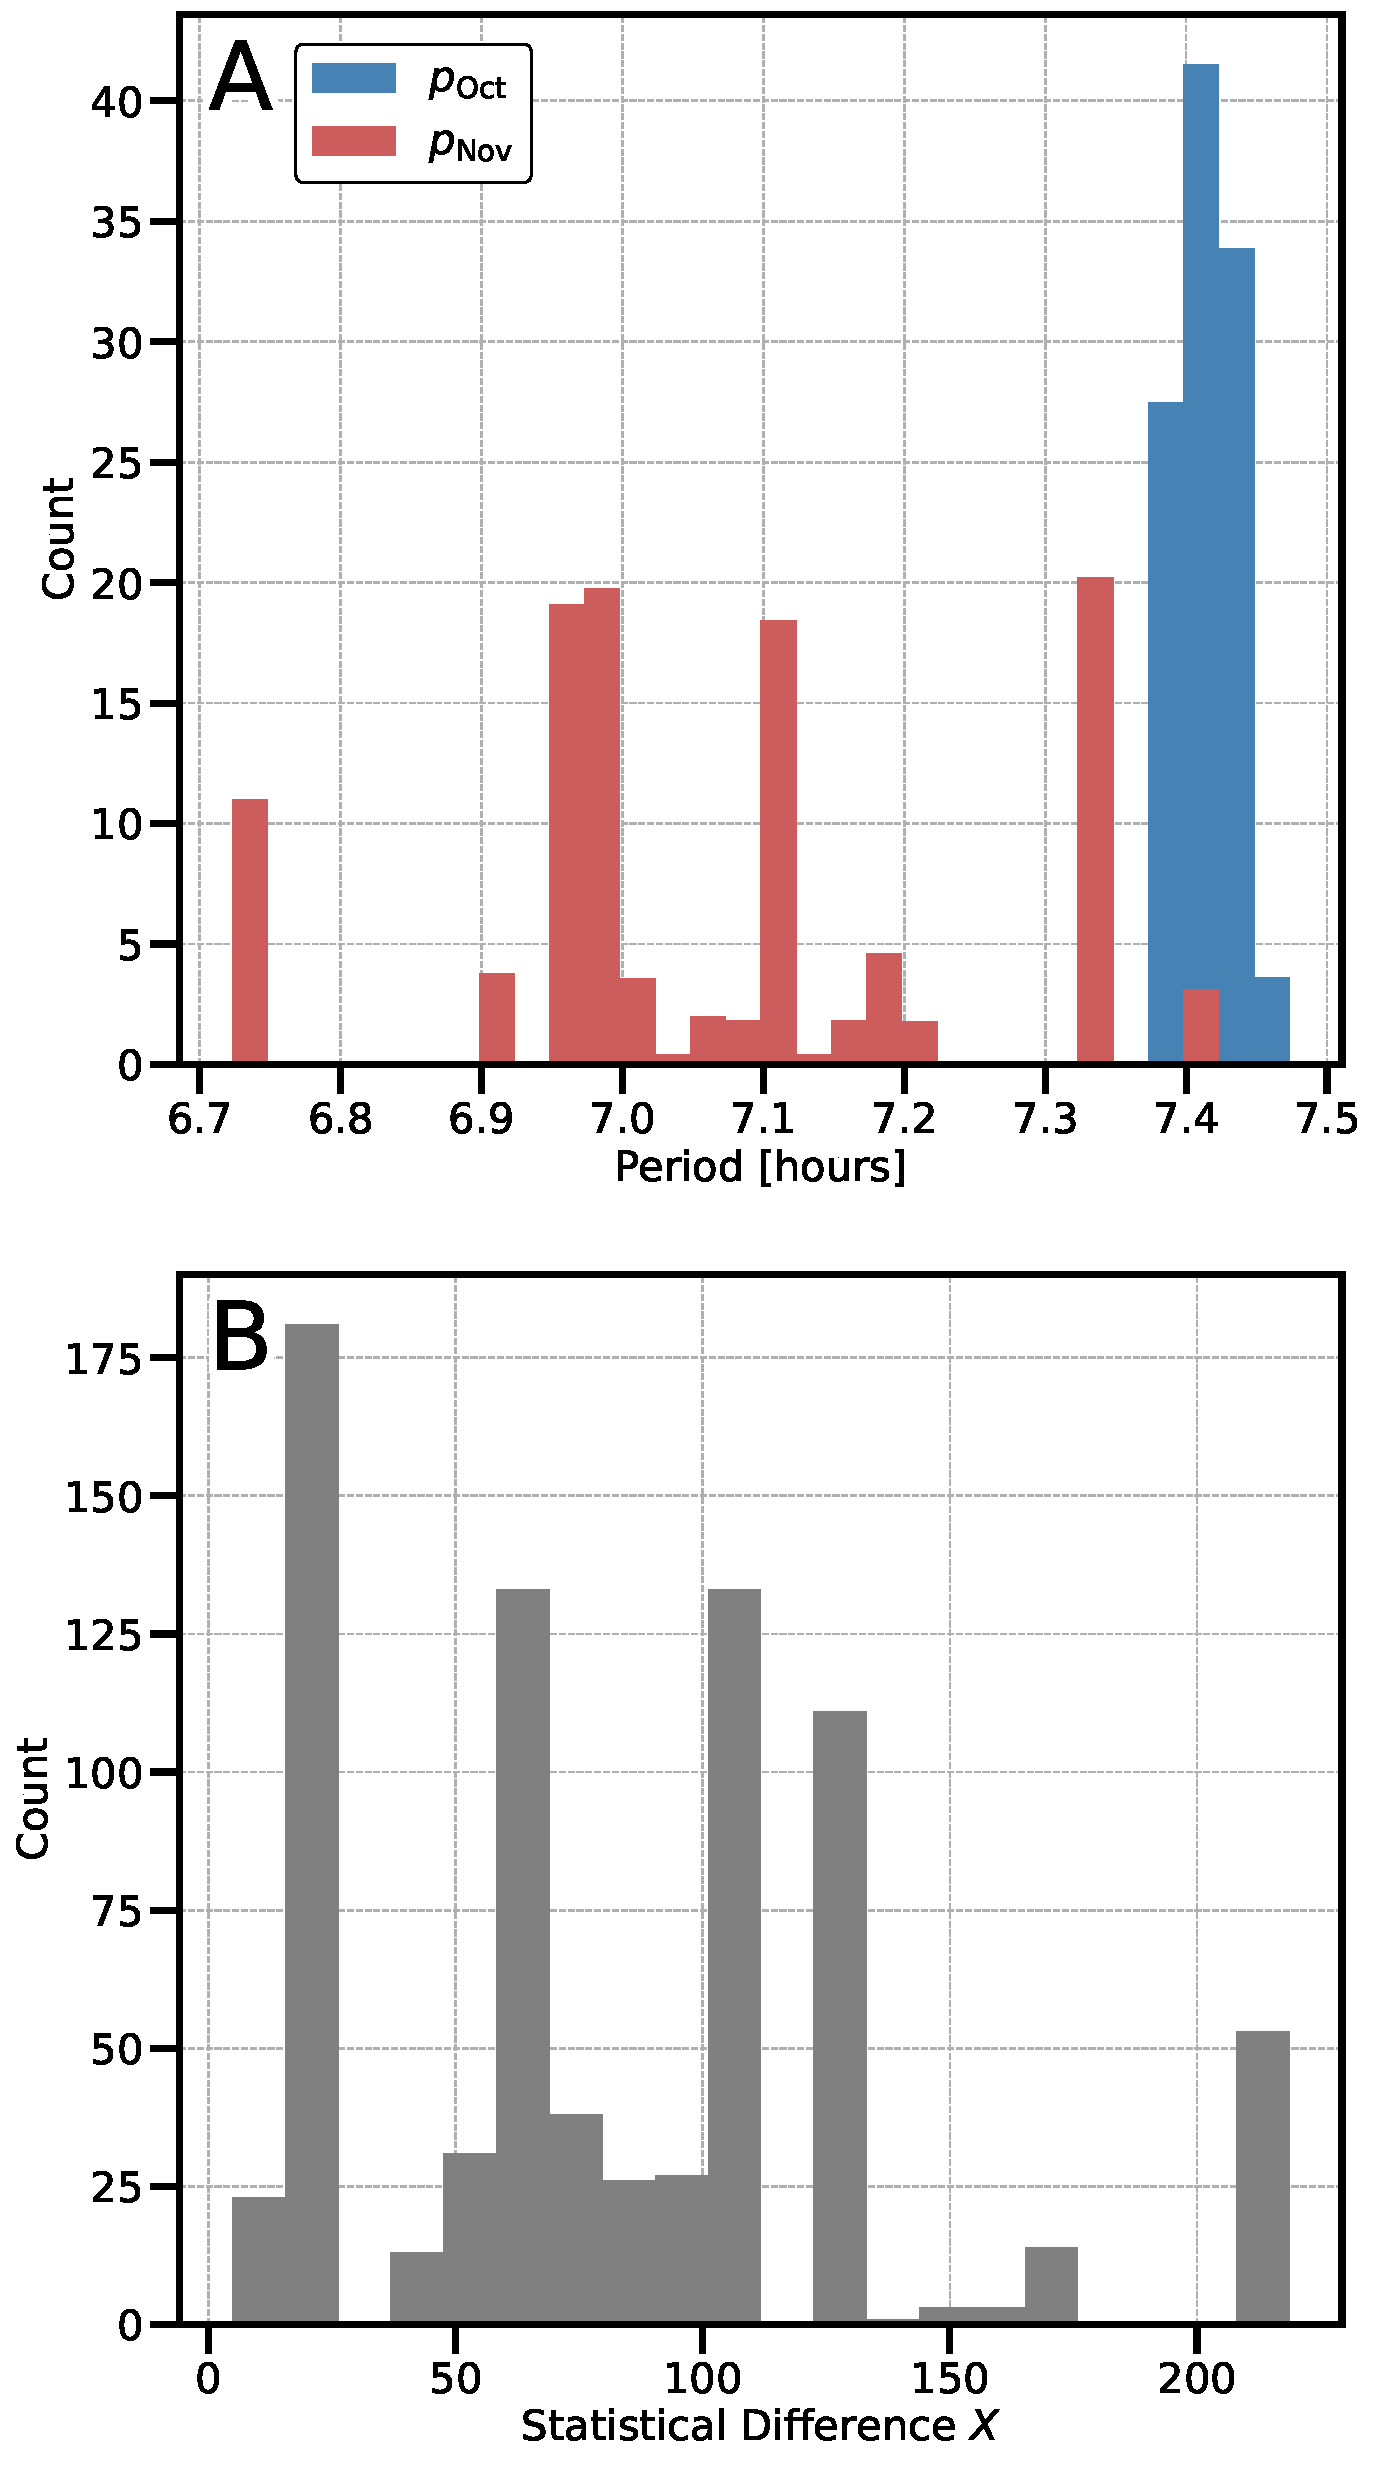
\includegraphics[width=\linewidth,angle=0]{period_comp_hist.pdf}
    \caption{ Histograms of (A) the computed October and November periods and (B) the statistical difference between each October and November period pair.}
    \label{fig:percomphist}
\end{figure}

To identify potential changes in the rotational period, we perform a similar meta-optimization for data obtained during 2017 November 21-23. Here, we optimize all parameters except $\theta$, $\phi$, and $\psi$, which are held constant. We compute the statistical difference $X$ between the October and November periods identified with this method, although we only include high-quality fits in the comparison by restricting $\chi^2<$30,000. The statistical difference is computed between paired data as $X=|p_\text{Oct}-p_\text{Nov}|/\sqrt{\sigma_\text{Oct}^2+\sigma_\text{Nov}^2}$, where $p_{\rm Oct}$, $p_{\rm Nov}$ are the periods fit to the October and November data and $\sigma_\text{Oct},\,\sigma_\text{Nov}$ are the uncertainties in the periods. Histograms of the identified periods and their corresponding statistical difference are shown in Figure \ref{fig:percomphist}. 

\begin{figure}
\centering
    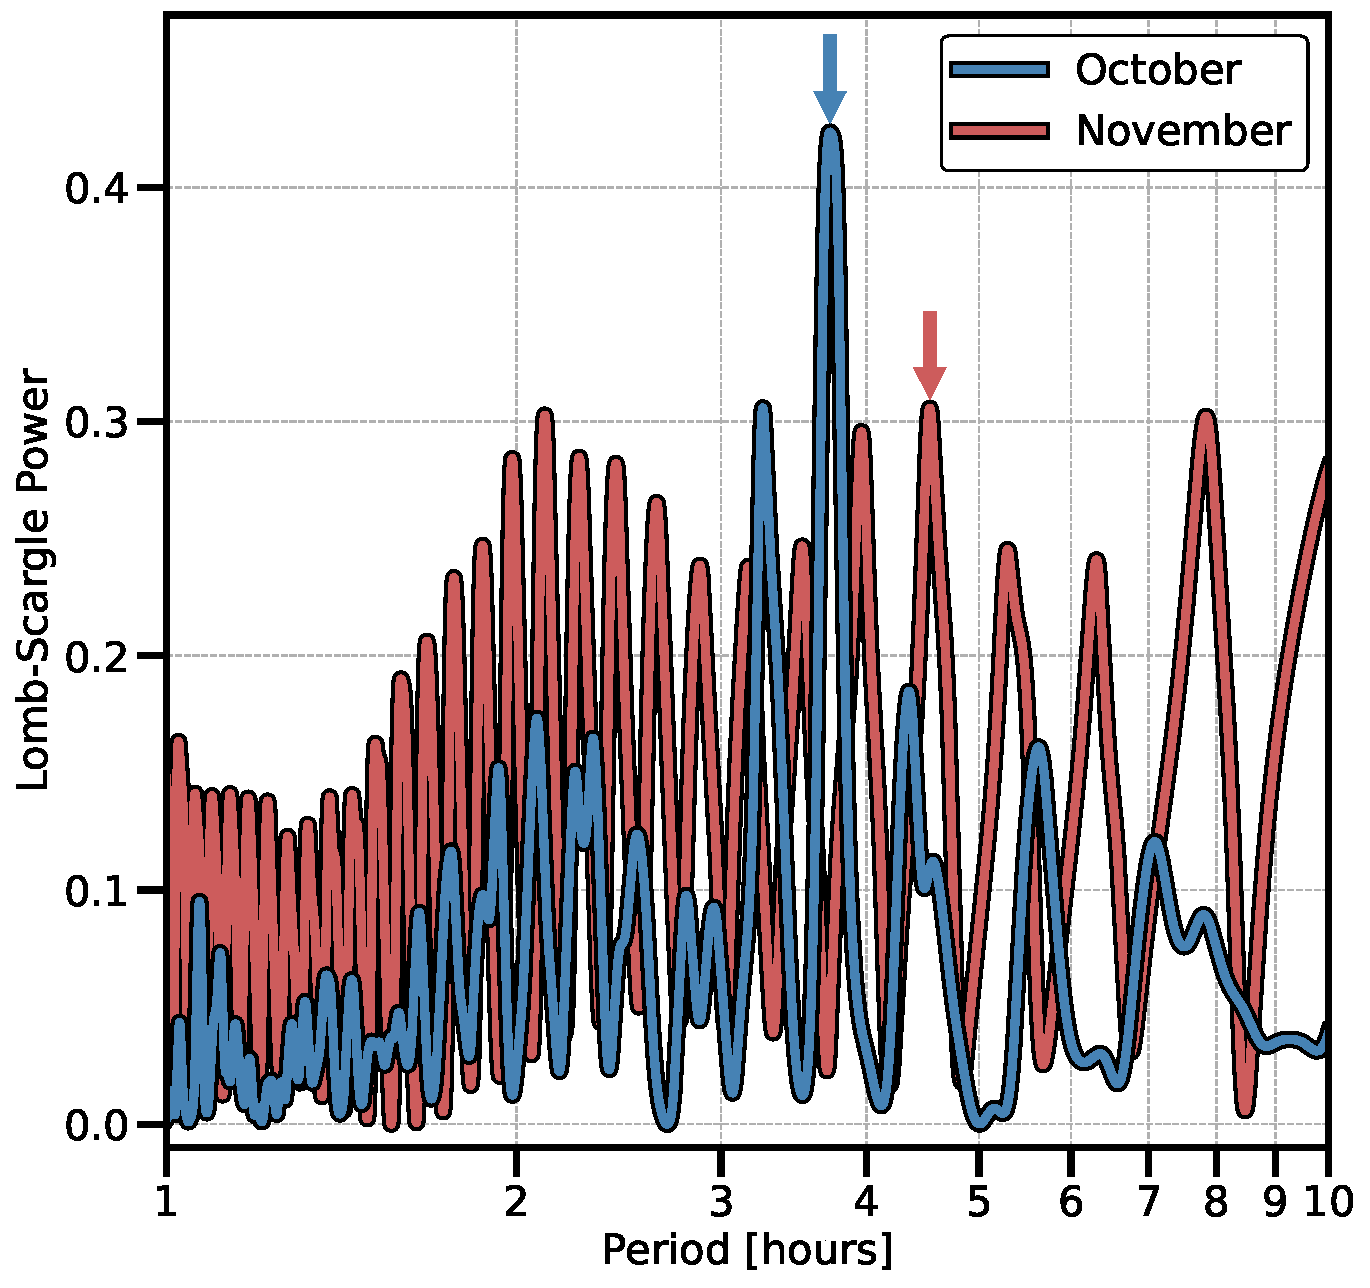
\includegraphics[width=\linewidth,angle=0]{lomb_scargle_power.pdf}
    \caption{Lomb-Scargle periodogram for the October 25-30 and November 21-23 data. Maxima are indicated with arrows.}
    \label{fig:lombscargle}
\end{figure}

The minimum statistical difference between two October-November periods is $X\simeq5\sigma$, while the maximum is $X\simeq219\sigma$. This is a significant detection of spin-up, further corroborated by the minimal overlap between the October and November histograms. The optimal fit to the October and November nights have periods $p=7.3975\pm1.11\cdot10^{-3}$ and $p_\text{Nov}=7.1910\pm9.84\cdot10^{-3}$ respectively, with $X\simeq21\sigma$. 

\begin{figure*}
    \centering
    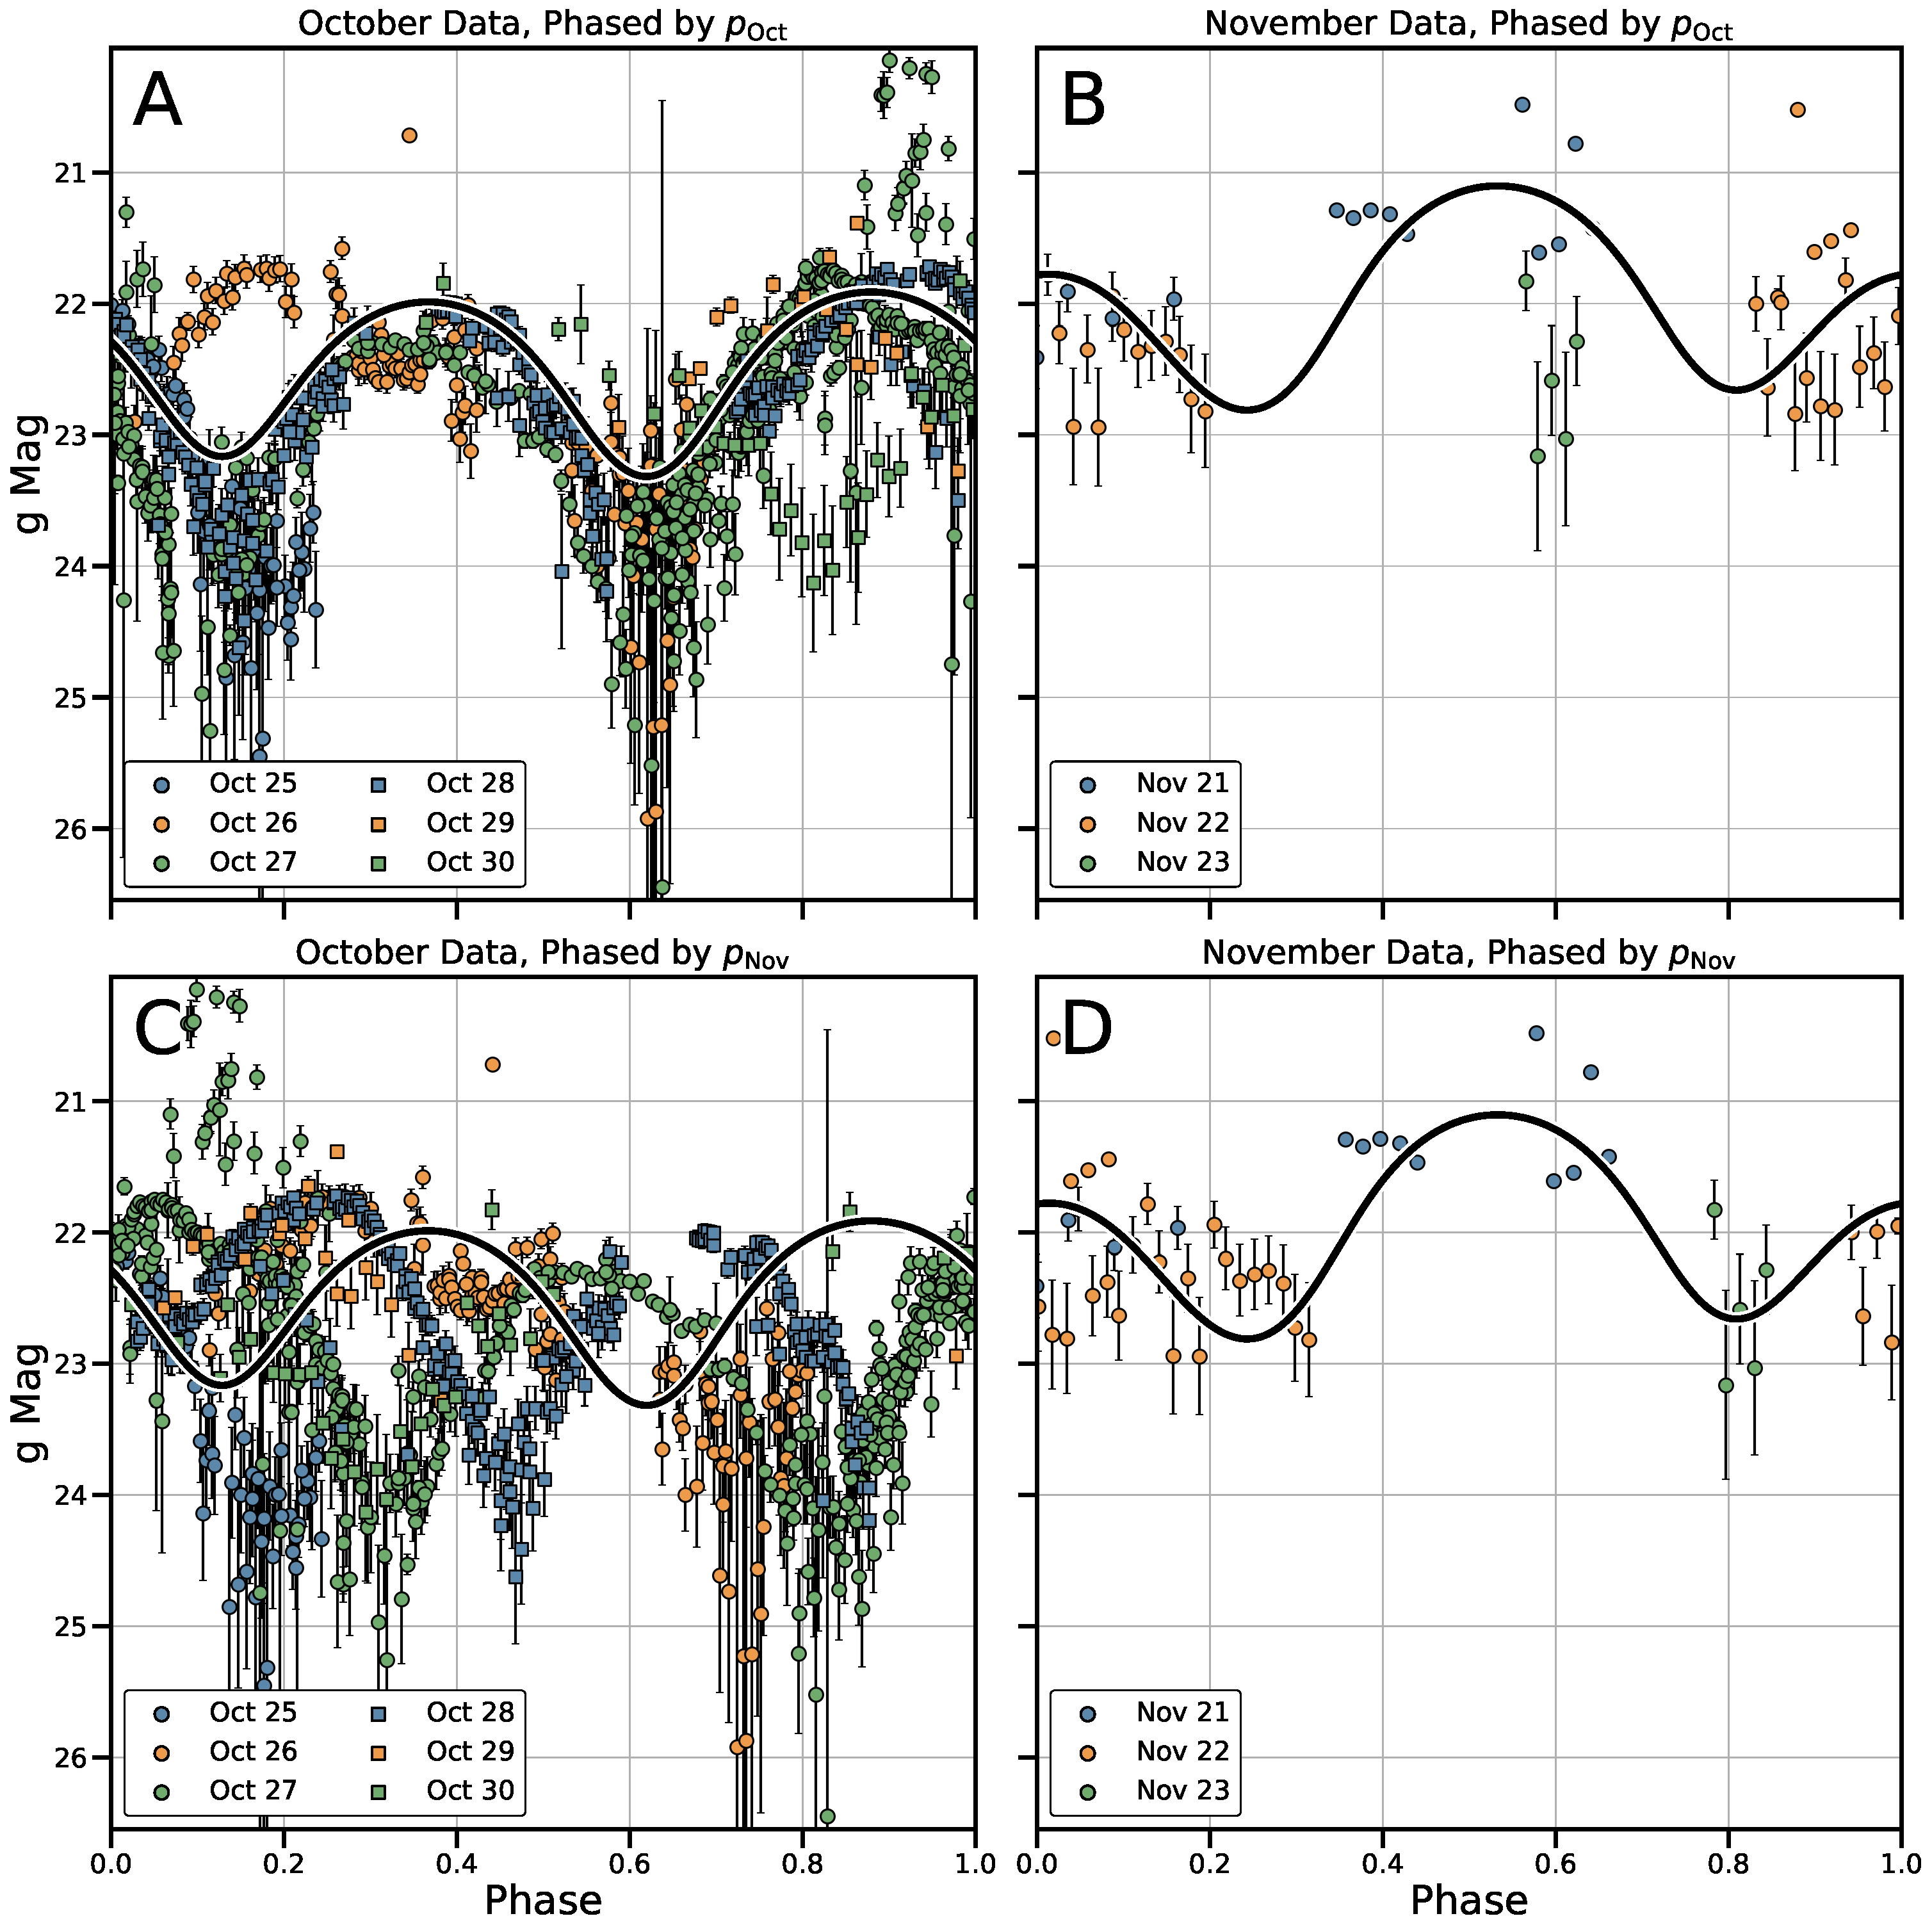
\includegraphics[width=\textwidth,angle=0]{phased_lightcurve.pdf}
    \caption{A comparison of the best fitting October and November periods with phase folded synthetic light curves and data. The points are color coded by date. A) October 25-30 data phased by October 25-29 period. B) November 21-23 data phased by October 25-29 period. C) October 25-30 data phased by November 21-23 period. D) November 21-23 data phased by November 21-23 period.}
    \label{fig:phasedcurve}
\end{figure*}

We compute Lomb-Scargle periodograms \citep{lomb1976,scargle1982} of the October and November data (Figure \ref{fig:lombscargle}) using the \texttt{astropy.timeseries.LombScargle} class \citep{astropy1,astropy2}, over a period domain of $[1,10]$ hours. There is a clear difference between both periodograms --- while the October periodogram exhibits a $1/2$ harmonic maximum at $p\simeq4$ hours, the November periodogram exhibits no obvious maxima. The lack of maxima is likely caused by the sparse sampling of data available in November, which creates artificial periods. Curiously, the October maxima correspond to November minima, further demonstrating the change in `Oumuamua's spin period between October and November.

In Figure \ref{fig:phasedcurve}, we present the photometric data phase folded by the best-fitting October and November periods, $p_\text{Oct}$ and $p_\text{Nov}$. $p_\text{Oct}$ is a significantly better fit to the October data than $p_\text{Nov}$ (Figure \ref{fig:phasedcurve}A and \ref{fig:phasedcurve}C); similarly, $p_\text{Nov}$ is a better fit to the November nights than $p_\text{Oct}$ (Figure \ref{fig:phasedcurve}B and \ref{fig:phasedcurve}D). Comparisons of these phased data further corroborate the change in spin period between October and November, and are not simply a manifestation of a paucity of data in November.

\subsection{Resolving Tension with Existing Work}\label{sec:flekkoyana}

In this subsection, we attempt to resolve the contradiction between this identified spin-up and the spin-down reported by \citet{flekkoy2019}. Firstly, that analysis used data from a variety of sources, sorted into authorial categories. The data quantity, quality, and cadence therefore vary between each observational campaign (whose lengths vary from 1-2 days). Further, different methodologies were used to compute the period in each study, making direct comparison difficult. 

The spin-down reported by \citet{flekkoy2019} was only detected during October. Therefore, it appears that `Oumuamua exhibited a slight spin-down during the October nights and a secular spin-up from October to November. Such a long-term spin-up due to outgassing torques is a well established effect \citep{Kokotanekova2018,Jewitt2021} which contributes to disintegration \citep{Jewitt2022} and fading \citep{brasser2015}. \citet{rafikov2018b} argued that `Oumuamua should have experienced significant spin-up from outgassing torques, consistent with this secular spin up. \citet{SLB2019} demonstrated that idealized arrangements of outgassing jets cause rotation without significant spin-up, which may explain the short-term lack of spin up in October.

It is also possible that tidal forces deformed `Oumuamua and changed the moment of inertia slightly. If this occurred, it could potentially affect either the amplitude of the light curve and the rotational period. While tidal forces are weaker than outgassing forces, it is plausible that deformation moderated the outgassing spin-up during October. `Oumuamua was closer to the Sun in October than it was in November, and the tidal forces were therefore stronger. With this motivation, we explore this possibility for the remainder of this paper.

\begin{figure}
\centering
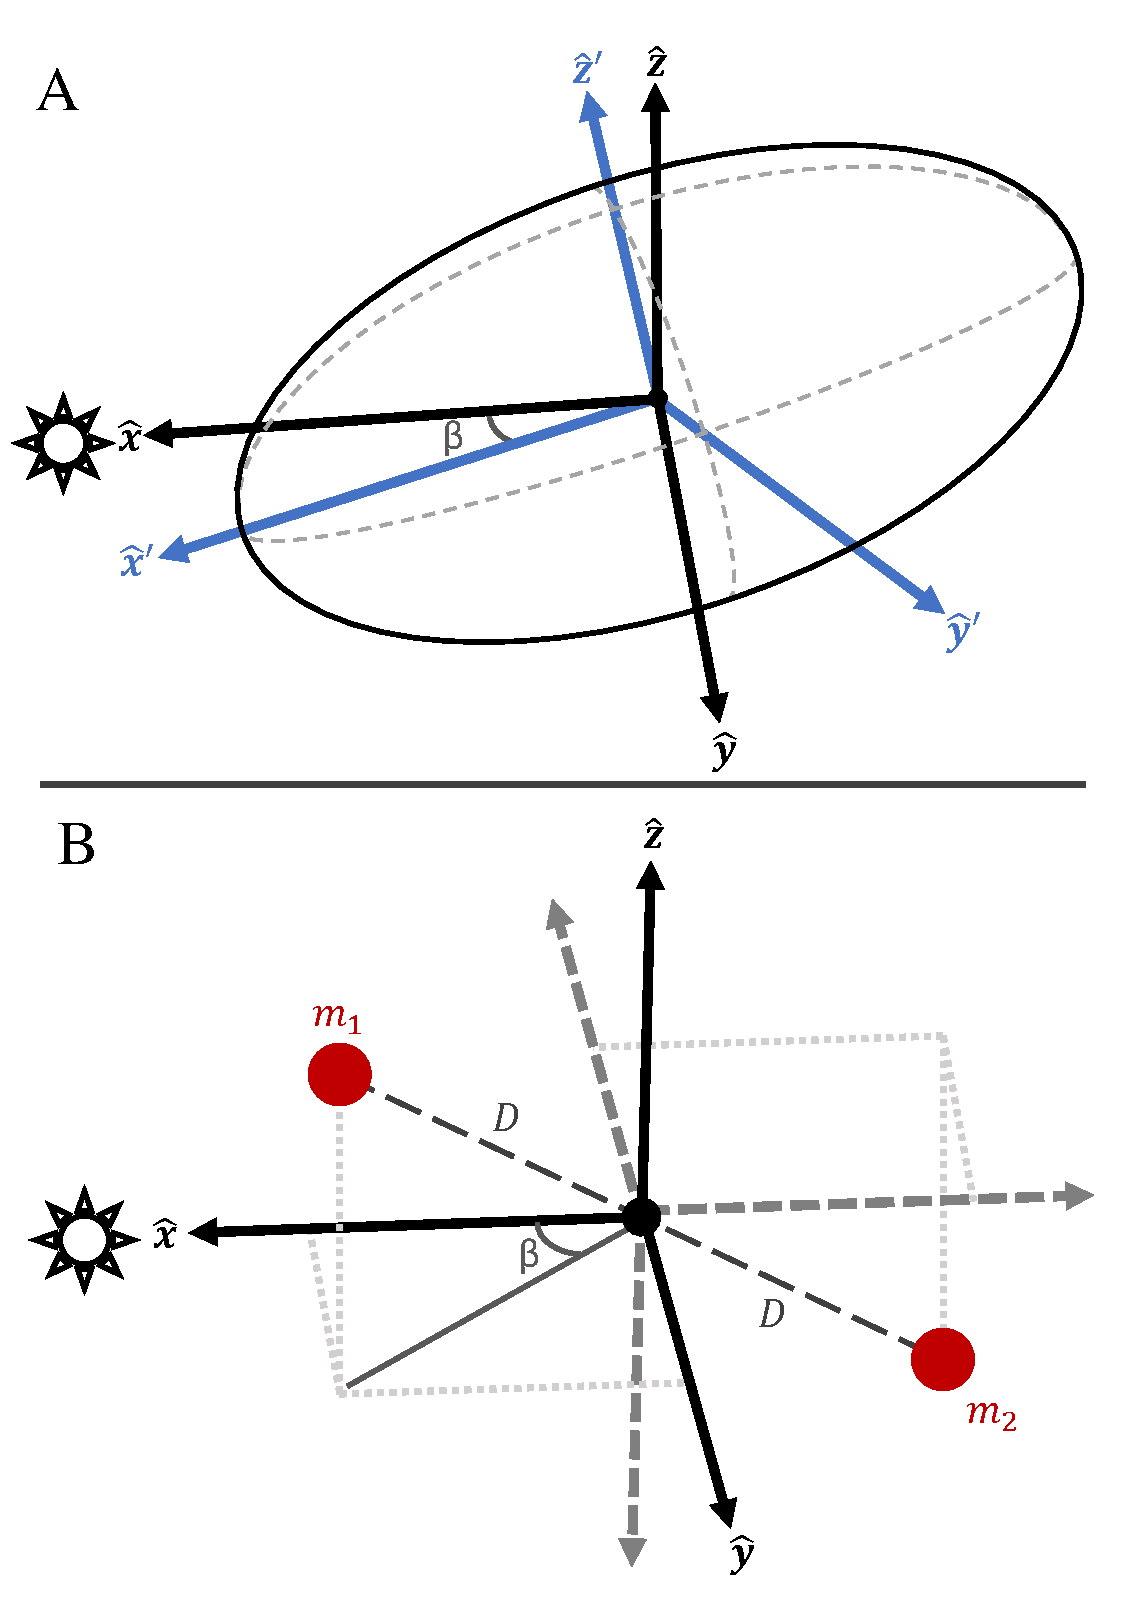
\includegraphics[width=\linewidth,angle=0]{dumbbellmodel.pdf}
\caption{Idealized models of an elongated object with primed and unprimed axes shown. A) Ellipsoid model and B) Dumbbell model.}
\label{fig:object_model}
\end{figure}

\section{Comparison of Outgassing and Tidal Torques}\label{sec:bigana}

In this section, we compare the effects of tidal and outgassing induced torques. In \S\ref{sec:tidana} and \S\ref{sec:jetana}, we calculate the magnitudes of each individual effect, which we compare in \S\ref{sec:torquecomp}. In \S\ref{sec:angleana}, we repeat this analysis with a more complex outgassing model. Mathematica files producing each of the equations presented here are publicly available at \url{https://github.com/astertaylor/Oumuamua}. 

\subsection{Tidal Torques}\label{sec:tidana}

In this subsection, we calculate the effect of tidal forces on `Oumuamua's rotation. We assume the body is an ellipsoid with semi-major axes $(a,b,c)$, $a=b,a>c$, and aspect ratio $\epsilon\equiv c/a$. We approximate the permanent quadrupole moment of the object as two concentric point masses of mass $m$ at a distance $D$ from the center of mass, similar to the ``dumbbell" model developed by \citet{Batygin2015} and \citet{Seligman2021_spin}. The use of this model is validated in Appendix \ref{sec:dumbval}.

We calculate values of $m$ and $D$ which reproduce the quadrupole moment of an ellipsoid. With the point masses located at $\pm(x,y,z)$, the dumbbell model has a quadrupole moment $Q_D$ given by 
\begin{equation}\label{eq:dumbbellquad}
Q_D=m \begin{pmatrix}
2x^2-y^2-z^2 & 0 & 0\\
0 & 2y^2-x^2-z^2 & 0\\
0 & 0 & 2z^2-x^2-y^2
\end{pmatrix}\,.
\end{equation} 
The quadrupole moment of an ellipsoid $Q_E$ is given by
\begin{equation}\label{eq:ellipsoidquad}
Q_E=\frac{M}{5}\begin{pmatrix}
2a^2-b^2-c^2 & 0 & 0\\
0 & 2b^2-a^2-c^2 & 0\\
0 & 0 & 2c^2-a^2-b^2
\end{pmatrix}\,,
\end{equation}
where $M=(4\pi/3)abc\rho$ is the total mass of the ellipsoid. 

By equating Equations \ref{eq:dumbbellquad} and \ref{eq:ellipsoidquad}, we find that the point masses are located at $\pm (R,R,0)$, where $R\equiv\sqrt{a^2-c^2}$. Therefore, $D=\sqrt{2}R$ and $m=(4\pi/15)abc\rho$. Schematic diagrams of this configuration are shown in Figure \ref{fig:object_model}. It is worth noting that for $a<c$, the point positions are distinct but the torques are equal (Appendix \ref{sec:cigtor}). 

We now provide a brief overview of the coordinate systems used in this section, although they are identical to those defined in \S \ref{sec:simplemodel}. The x-axis is the direction towards the Sun; the unprimed axes do not rotate with `Oumuamua. The object rotates about the y-axis by an angle $\beta$ with respect to the x-axis. The primed axes co-rotate with the body and align with its three principal axes. 

The two point masses, denoted by $m_1$ and $m_2$, are located at
\begin{equation}\label{eq:dumbbellpts}
    \begin{dcases}
    +\,R\,\big(\cos\beta\,\boldsymbol{\hat{x}'}+\boldsymbol{\hat{y}'}-\sin\beta\,\boldsymbol{\hat{z}'}\big), &\text{for $m_1$}\\
    -\,R\,\big(\cos\beta\,\boldsymbol{\hat{x}'}+\boldsymbol{\hat{y}'}-\sin\beta\,\boldsymbol{\hat{z}'}\big), &\text{for $m_2$}\,.
    \end{dcases}
\end{equation}
At a heliocentric distance $r_H$, the acceleration on the center of mass $\boldsymbol{a}_{\text{COM}}$ is given by
\begin{equation}\label{eq:comacc}
    \boldsymbol{a}_{\text{COM}}=-\bigg(\frac{G M_{\Sun}}{r_H^2}\bigg)\,\boldsymbol{\hat{x}}\,,
\end{equation} 
while the acceleration of each of the point masses is given by
\begin{equation}
    \begin{dcases}
    \boldsymbol{a}_{m_1}=-\,\bigg(\,\frac{G M_{\Sun}}{\left(r_H-R\cos{\beta}\right)^2}\,\bigg)\,\boldsymbol{\hat{x}}\\
    \boldsymbol{a}_{m_2}=-\,\bigg(\,\frac{G M_{\Sun}}{\left(r_H+R\cos{\beta})\right)^2}\,\bigg)\,\boldsymbol{\hat{x}}\,.
    \end{dcases}
\end{equation} 
The tidal acceleration is the difference in these accelerations, and so the force is simply
\begin{equation}\label{eq:torqueforce}
    \begin{dcases}
    \boldsymbol{F}_{\text{tidal}}(m_1)=-\,G M_{\Sun}m \bigg(\,\frac{1}{\left(r_H-R\cos{\beta}\right)^2}-\frac{1}{r_H^2}\, \bigg)\,\boldsymbol{\hat{x}}\\
    \boldsymbol{F}_{\text{tidal}}(m_2)=-\,G M_{\Sun}m \bigg(\,\frac{1}{\left(r_H+R\cos{\beta}\right)^2}-\frac{1}{r_H^2}\, \bigg)\,\boldsymbol{\hat{x}}.
    \end{dcases}
\end{equation} 

The lever arm is given by Equation \ref{eq:dumbbellpts}, and the corresponding tidal torque is given by the cross product of Equations \ref{eq:dumbbellpts} and \ref{eq:torqueforce}. The vector component is $\mp R(\sin{\beta}\,\boldsymbol{\hat{y}}+\boldsymbol{\hat{z}})$, and we take only the y-component. The z-component of the torque arises from asymmetry across the x-axis in the `dumbbell' model not present in the ellipsoidal object and is ignored. The magnitude of the total torque about the y-axis is then 
\begin{equation}\label{eq:tidal}
    \tau_{\text{tidal}}=\frac{8\pi}{15}G M_{\Sun} \left( \frac{r_Ha^5\rho\epsilon(1-\epsilon^2)\sin(2\beta)}{\big(r_H^2- a^2(1-\epsilon^2)\cos^2{\beta}\big)^2} \right),
\end{equation} 
where we have substituted $a=b$, $R=\sqrt{a^2-c^2}$, $m=(4\pi/15)abc\rho$, and $\epsilon=c/a$. Notably, this is equivalent to the y- or z-axis rotating torque for a body with $b=c$ and $a>c$ (see Appendix \ref{sec:cigtor}).

\subsection{Outgassing Torques}\label{sec:jetana}

In this subsection, we calculate the magnitude of outgassing torques on `Oumuamua. The outgassing force is $M\,4.92\cdot10^{-4}\, (r_H)^{-2}\,\boldsymbol{\hat{r}}$ cm s$^{-2}$, with $r_H$ in au and $M$ the object mass \citep{micheli2018}. We assume this force operates at the substellar point and normal to the surface of the ellipsoidal body, as in \citet{SLB2019}.

Without loss of generality, we only consider the rotation about the y-axis. The rotation matrix $\boldsymbol{R}$, which transforms from the primed to the unprimed axes, is given by
\begin{equation}
    \boldsymbol{R}=\begin{pmatrix}
    \cos\beta & 0 & \sin\beta \\
    0 & 1 & 0\\
    -\sin\beta & 0 & \cos\beta
    \end{pmatrix}\,,
\end{equation} 
and the inverse is simply the transpose.

In the primed body frame, the equation of the ellipsoid is given by the relationship
\begin{equation}
    f_{\rm 3d}(x',y',z')=\frac{x'^2}{a^2}+\frac{y'^2}{b^2}+\frac{z'^2}{c^2}-1=0\,,
\end{equation}
and the unit vector normal to this surface is 
\begin{equation}\label{eq:norm}
    \frac{\nabla f_{\rm 3d}}{\|\nabla f_{\rm 3d}\|}=\left[\frac{x'^2}{a^4}+\frac{y'^2}{b^4}+\frac{z'^2}{c^4}\right]^{-1/2}\left[\frac{x'}{a^2}\boldsymbol{\hat{x}}+\frac{y'}{b^2}\boldsymbol{\hat{y}}+\frac{z'}{c^2}\boldsymbol{\hat{z}}\right]. 
\end{equation}
We further define a normalization factor, $f$, to be
\begin{equation}\label{eq:f_def}
    f\equiv\sqrt{(a\cos\beta)^2+(c\sin\beta)^2}\,.
\end{equation} 
Then the position of the substellar point, $(x_{ss}',y_{ss}',z_{ss}')$, is located where Equation \ref{eq:norm} is equal to $\boldsymbol{R}^{-1}\boldsymbol{\hat{x}}$, at
\begin{equation}
\begin{aligned}
\begin{dcases}
  x_{ss}'=\pm a^2\cos\beta/f\\
  y_{ss}'=0\\ 
  z_{ss}'=\pm c^2\sin\beta/f 
\end{dcases}\,,
\end{aligned}
\end{equation} 
under the condition that
\begin{equation}\label{eq:ellcondition}
    \cos(\beta)x_{ss}'/a^2+\sin(\beta)z_{ss}'/c^2<0\,.
\end{equation}

Substituting ($x'_{ss}$, $y'_{ss}$, $z'_{ss}$) into Equation \ref{eq:ellcondition}, we choose the negative variant to ensure that the outgassing jet points towards the Sun rather than away. $f$ is positive, so 
\begin{equation}\label{eq:ssprimepoints}
\begin{aligned}
\begin{dcases}
    x_{ss}'=-a^2\cos\beta/f\\
    y_{ss}'= 0 \\ 
    z_{ss}'=-c^2\sin\beta/f.
\end{dcases}
\end{aligned}
\end{equation}

We now rotate this point to the unprimed substellar point $(x_{ss},\,y_{ss},\,z_{ss})$ using the rotation matrix $\boldsymbol{R}$. The torque is then given by the cross product of the substellar points with the force, so
\begin{equation}\label{eq:jetvec}
\begin{aligned}
    \boldsymbol{\tau}=&MA_{ng}\left(\frac{\sin(2\theta)}{2f}(a^2-c^2)\right)\hat{\mathbf{y}}.
\end{aligned}
\end{equation}
Recall that $M=(4\pi/3)abc\rho$, $A_{ng}=4.92\cdot10^{-4}\,r_H^{-2}$ cm s$^{-2}$, with $r_H$ in au. We then define $B=1.101\cdot10^{23}$ cm$^3$ s$^{-2}$ (in cgs) such that $A_{ng}=B\, r_H^{-2}$. The magnitude of the outgassing torque which operates along the y-axis $\tau_{\text{jet}}$ is then finally given by
\begin{equation}\label{eq:jet}
\begin{aligned}
    \tau_{\text{jet}}=\,\bigg(\,\frac{2\pi}{3}Ba^4\rho\,\bigg)\,\bigg( \frac{\epsilon(1-\epsilon^2)\sin(2\beta)}{r_H^2\sqrt{\cos^2\beta+\epsilon^2\sin^2\beta}}\,\bigg)\,.
\end{aligned}
\end{equation}

\begin{figure}
    \centering
    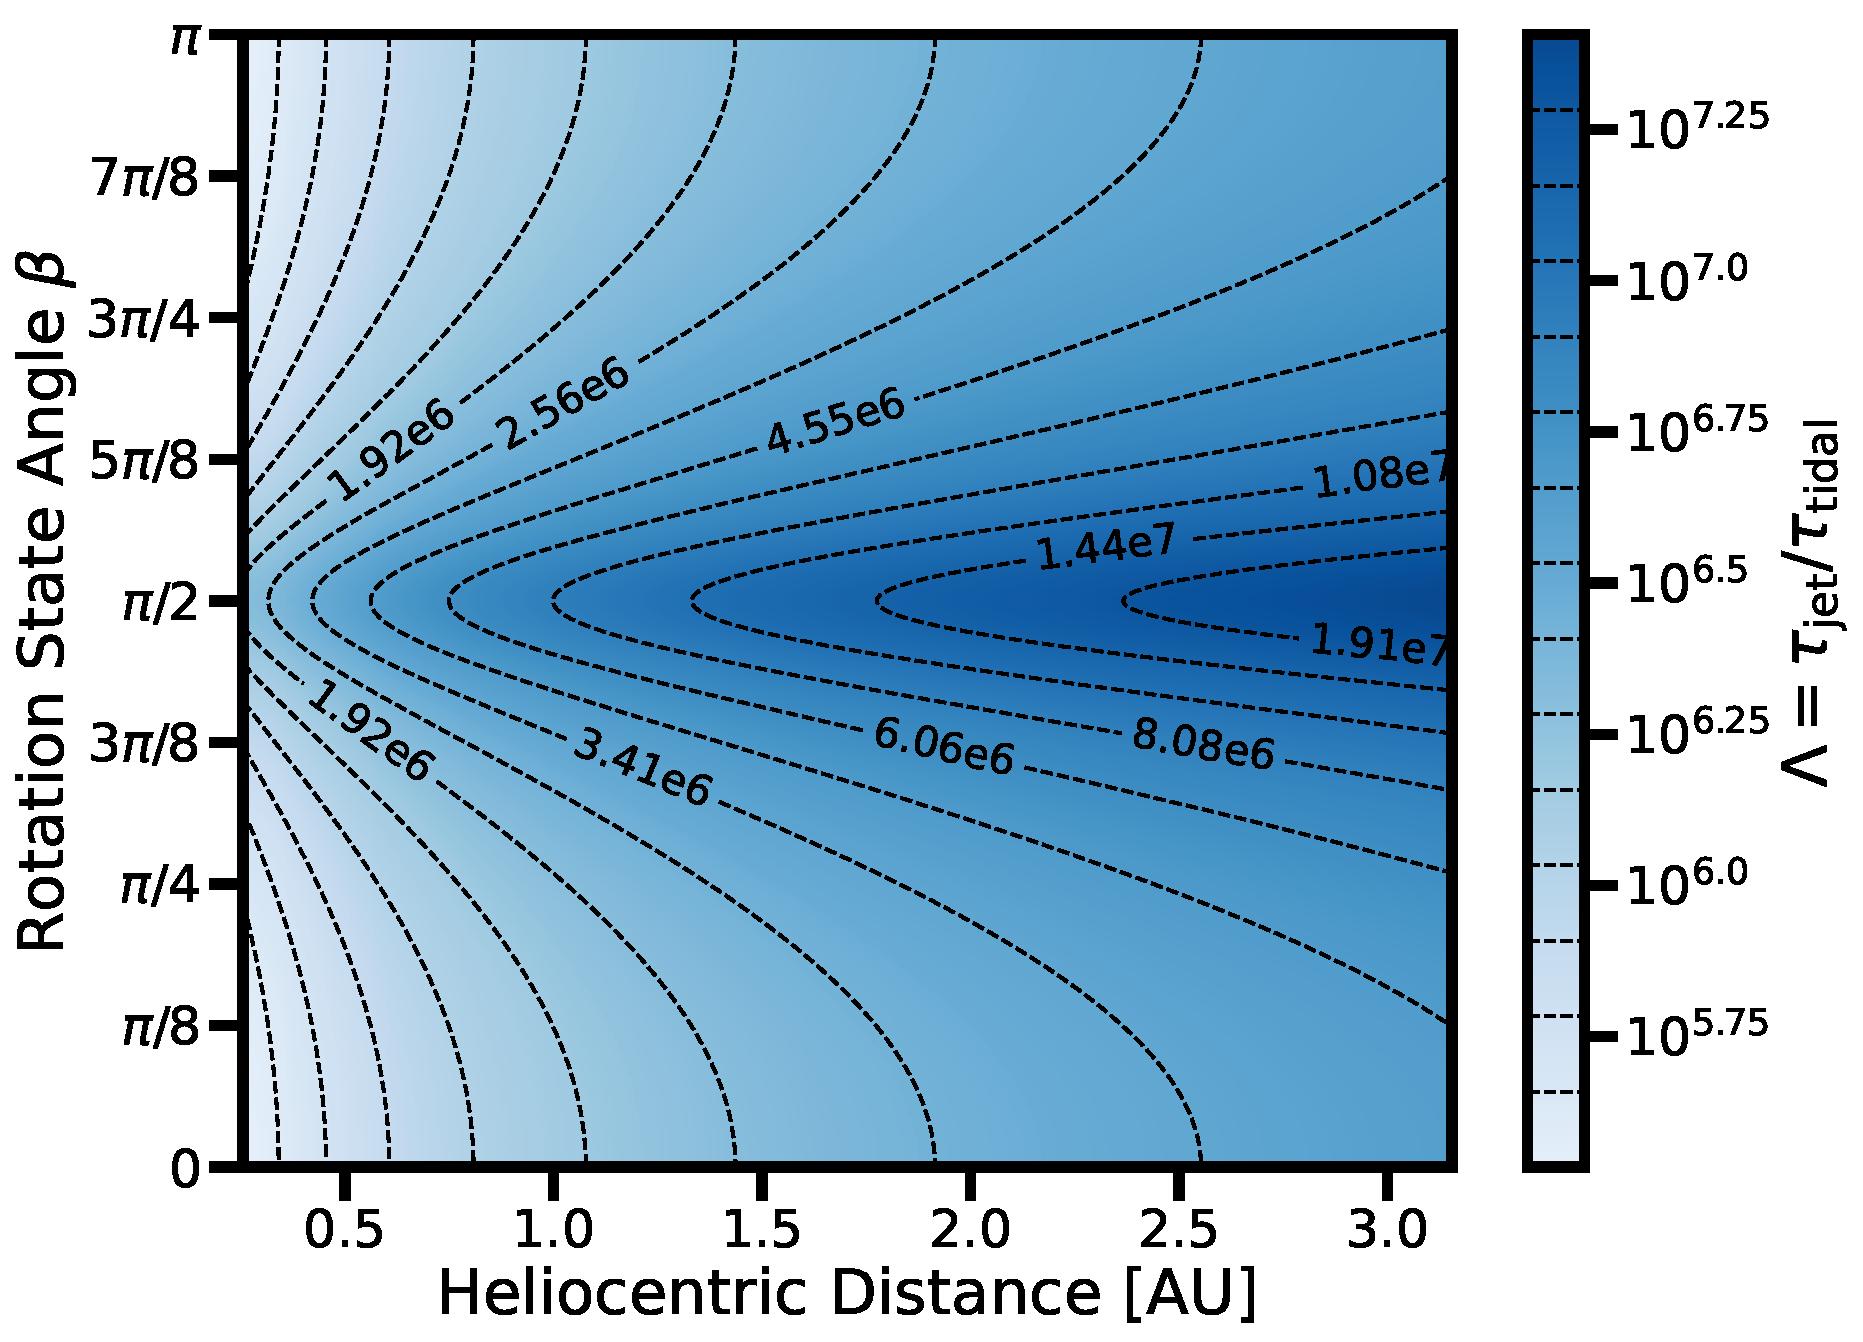
\includegraphics[width=\linewidth,angle=0]{torque_ratio.pdf}
    \caption{The ratio of outgassing to tidal torques, with the color representing the ratio and the contours showing the shape of the ratio space.}
    \label{fig:analytic_ratio}
\end{figure}

\subsection{Comparison of Outgassing and Tidal Torque}\label{sec:torquecomp}

In this subsection, we compare the magnitudes of the outgassing and tidal torques. 

We define $\Lambda\equiv\tau_{\mathrm{jet}}/\tau_{\mathrm{tidal}}$, which can also be written as
\begin{equation}
    \Lambda(a,c,r_H,\theta)=\frac{5B}{4GM_\Sun}\left(\frac{(r_H^2-(a^2-c^2)\cos^2{\beta})^2}{r_H^3\sqrt{(a\cos\beta)^2+(c\sin\beta)^2}}\right)\,.
\end{equation}

The ratio of outgassing to tidal torques for a range of $r_H$ and $\beta$ is shown in Figure \ref{fig:analytic_ratio}. For these values, the maximum value of $\Lambda$ is $2.54\cdot10^7$, and the minimum value is $3.43\cdot10^5$. Clearly, the outgassing torque dominates the rotational dynamics under these idealized assumptions.

\begin{figure}
\centering
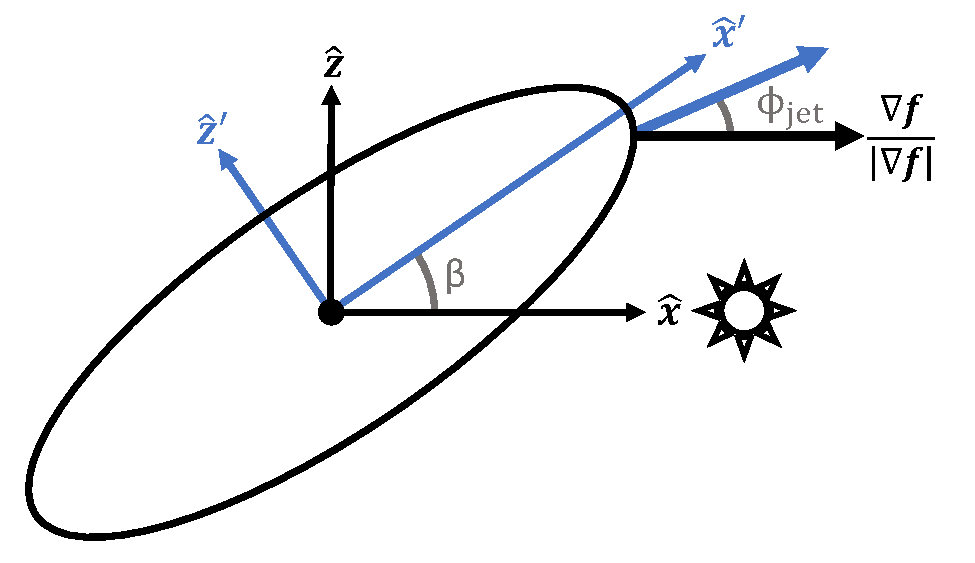
\includegraphics[width=\linewidth,angle=0]{outgassing_diagram.pdf}
\caption{Structure of the non-normal outgassing torques.}
\label{fig:outgas_rot}
\end{figure}

\subsection{Variations in Outgassing Angle}\label{sec:angleana}

In this subsection, we calculate the outgassing torque with more general assumptions. Specifically, we relax the assumption that the outgassing vents normal to the surface, instead setting the direction of the outgassing to be offset from the normal by an angle $\phi_{\rm jet}\in[-\pi/2,\pi/2]$ (Figure \ref{fig:outgas_rot}). The force is then along the direction $\boldsymbol{\hat{F}}=\cos{\phi_{\rm jet}}\,\boldsymbol{\hat{x}}+\sin{\phi_{\rm jet}}\,\boldsymbol{\hat{z}}$. 

We take the cross product of the substellar point ($x'_{ss}$, $y'_{ss}$, $z'_{ss}$) with this force to obtain the torque. We substitute Equations \ref{eq:ssprimepoints} and \ref{eq:f_def} to obtain the magnitude of the torque $\tau_{\text{rotjet}}$, given by
\begin{equation}\label{eq:rotjettorque}
\begin{split}
    \tau_{\text{rotjet}}=\,\bigg(\,\frac{2\pi}{3}\frac{\rho a^4\epsilon B}{r_H^2}\,\bigg)\,\bigg(\frac{(1-\epsilon^2)\sin(2\beta)}{\sqrt{\cos^2(\beta)+\epsilon^2\sin^2(\beta)}}\,\bigg)\,\cos\phi_{\rm jet}\\
    +\,\bigg(\, 2\,\sqrt{\cos^2(\beta)+\epsilon^2\sin^2(\beta)}\,\bigg)\, \sin\phi_{\rm jet}\,.
\end{split}
\end{equation}

\begin{figure}
\centering
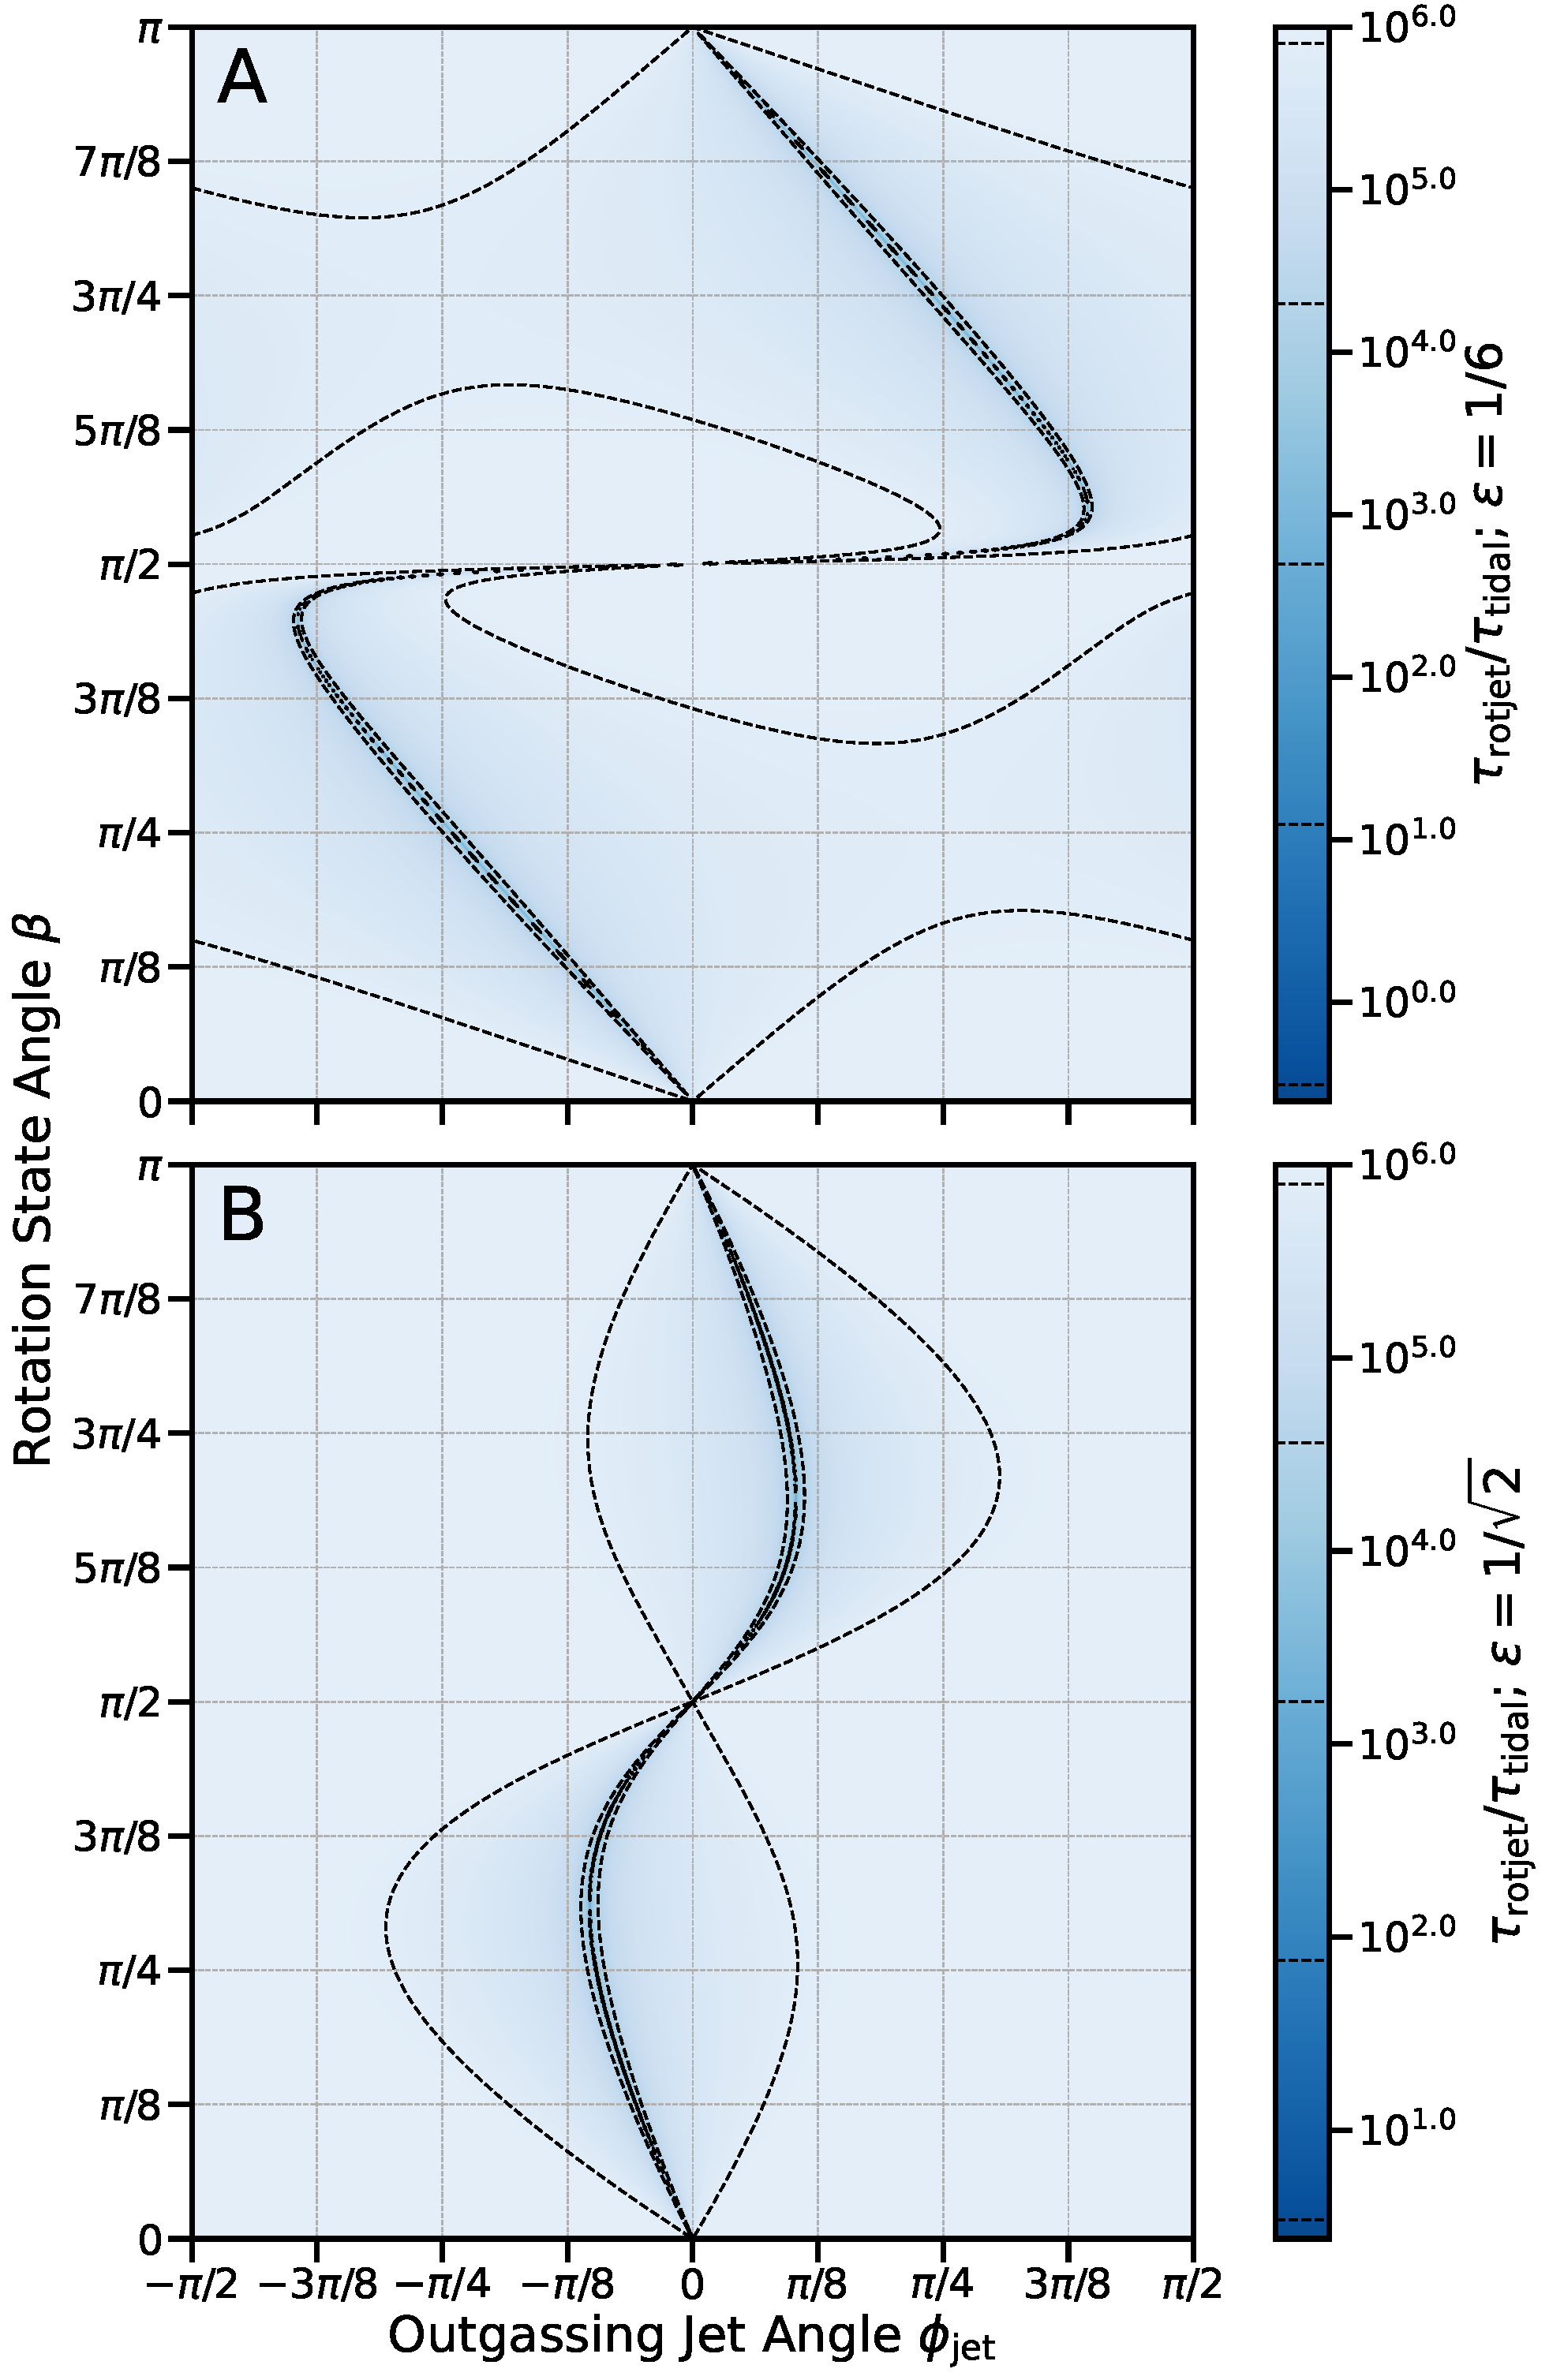
\includegraphics[width=\linewidth,angle=0]{rot_torque_ratio.pdf}
\caption{Ratio of the non-normal outgassing torque to the tidal torque (Equation \ref{eq:rotjettorque}), with $a=115$ m and $r_H=0.256$ au. A) $\epsilon=1/6$. B) $\epsilon=1/\sqrt{2}$.}
\label{fig:rot_ratio}
\end{figure}

In Figure \ref{fig:rot_ratio}, we show the magnitude of the ratio of the outgassing to tidal torque for a range of $\beta\in[0,\pi)$ and $\phi\in[-\pi/2,\pi/2]$, with $\epsilon=1/6,\sqrt{2}$ and $r_H=0.26$ au. For $\epsilon=1/6$, the minimum value of the ratio is $\Lambda\simeq 1/4$, at $(\beta,\, \phi_{\rm jet})=(0.83,-0.79)$. Therefore, while it is possible to construct a pathological scenario where both torques are comparable, the outgassing torque dominates the dynamics for most of the parameter space. 
\begin{figure*}
\centering
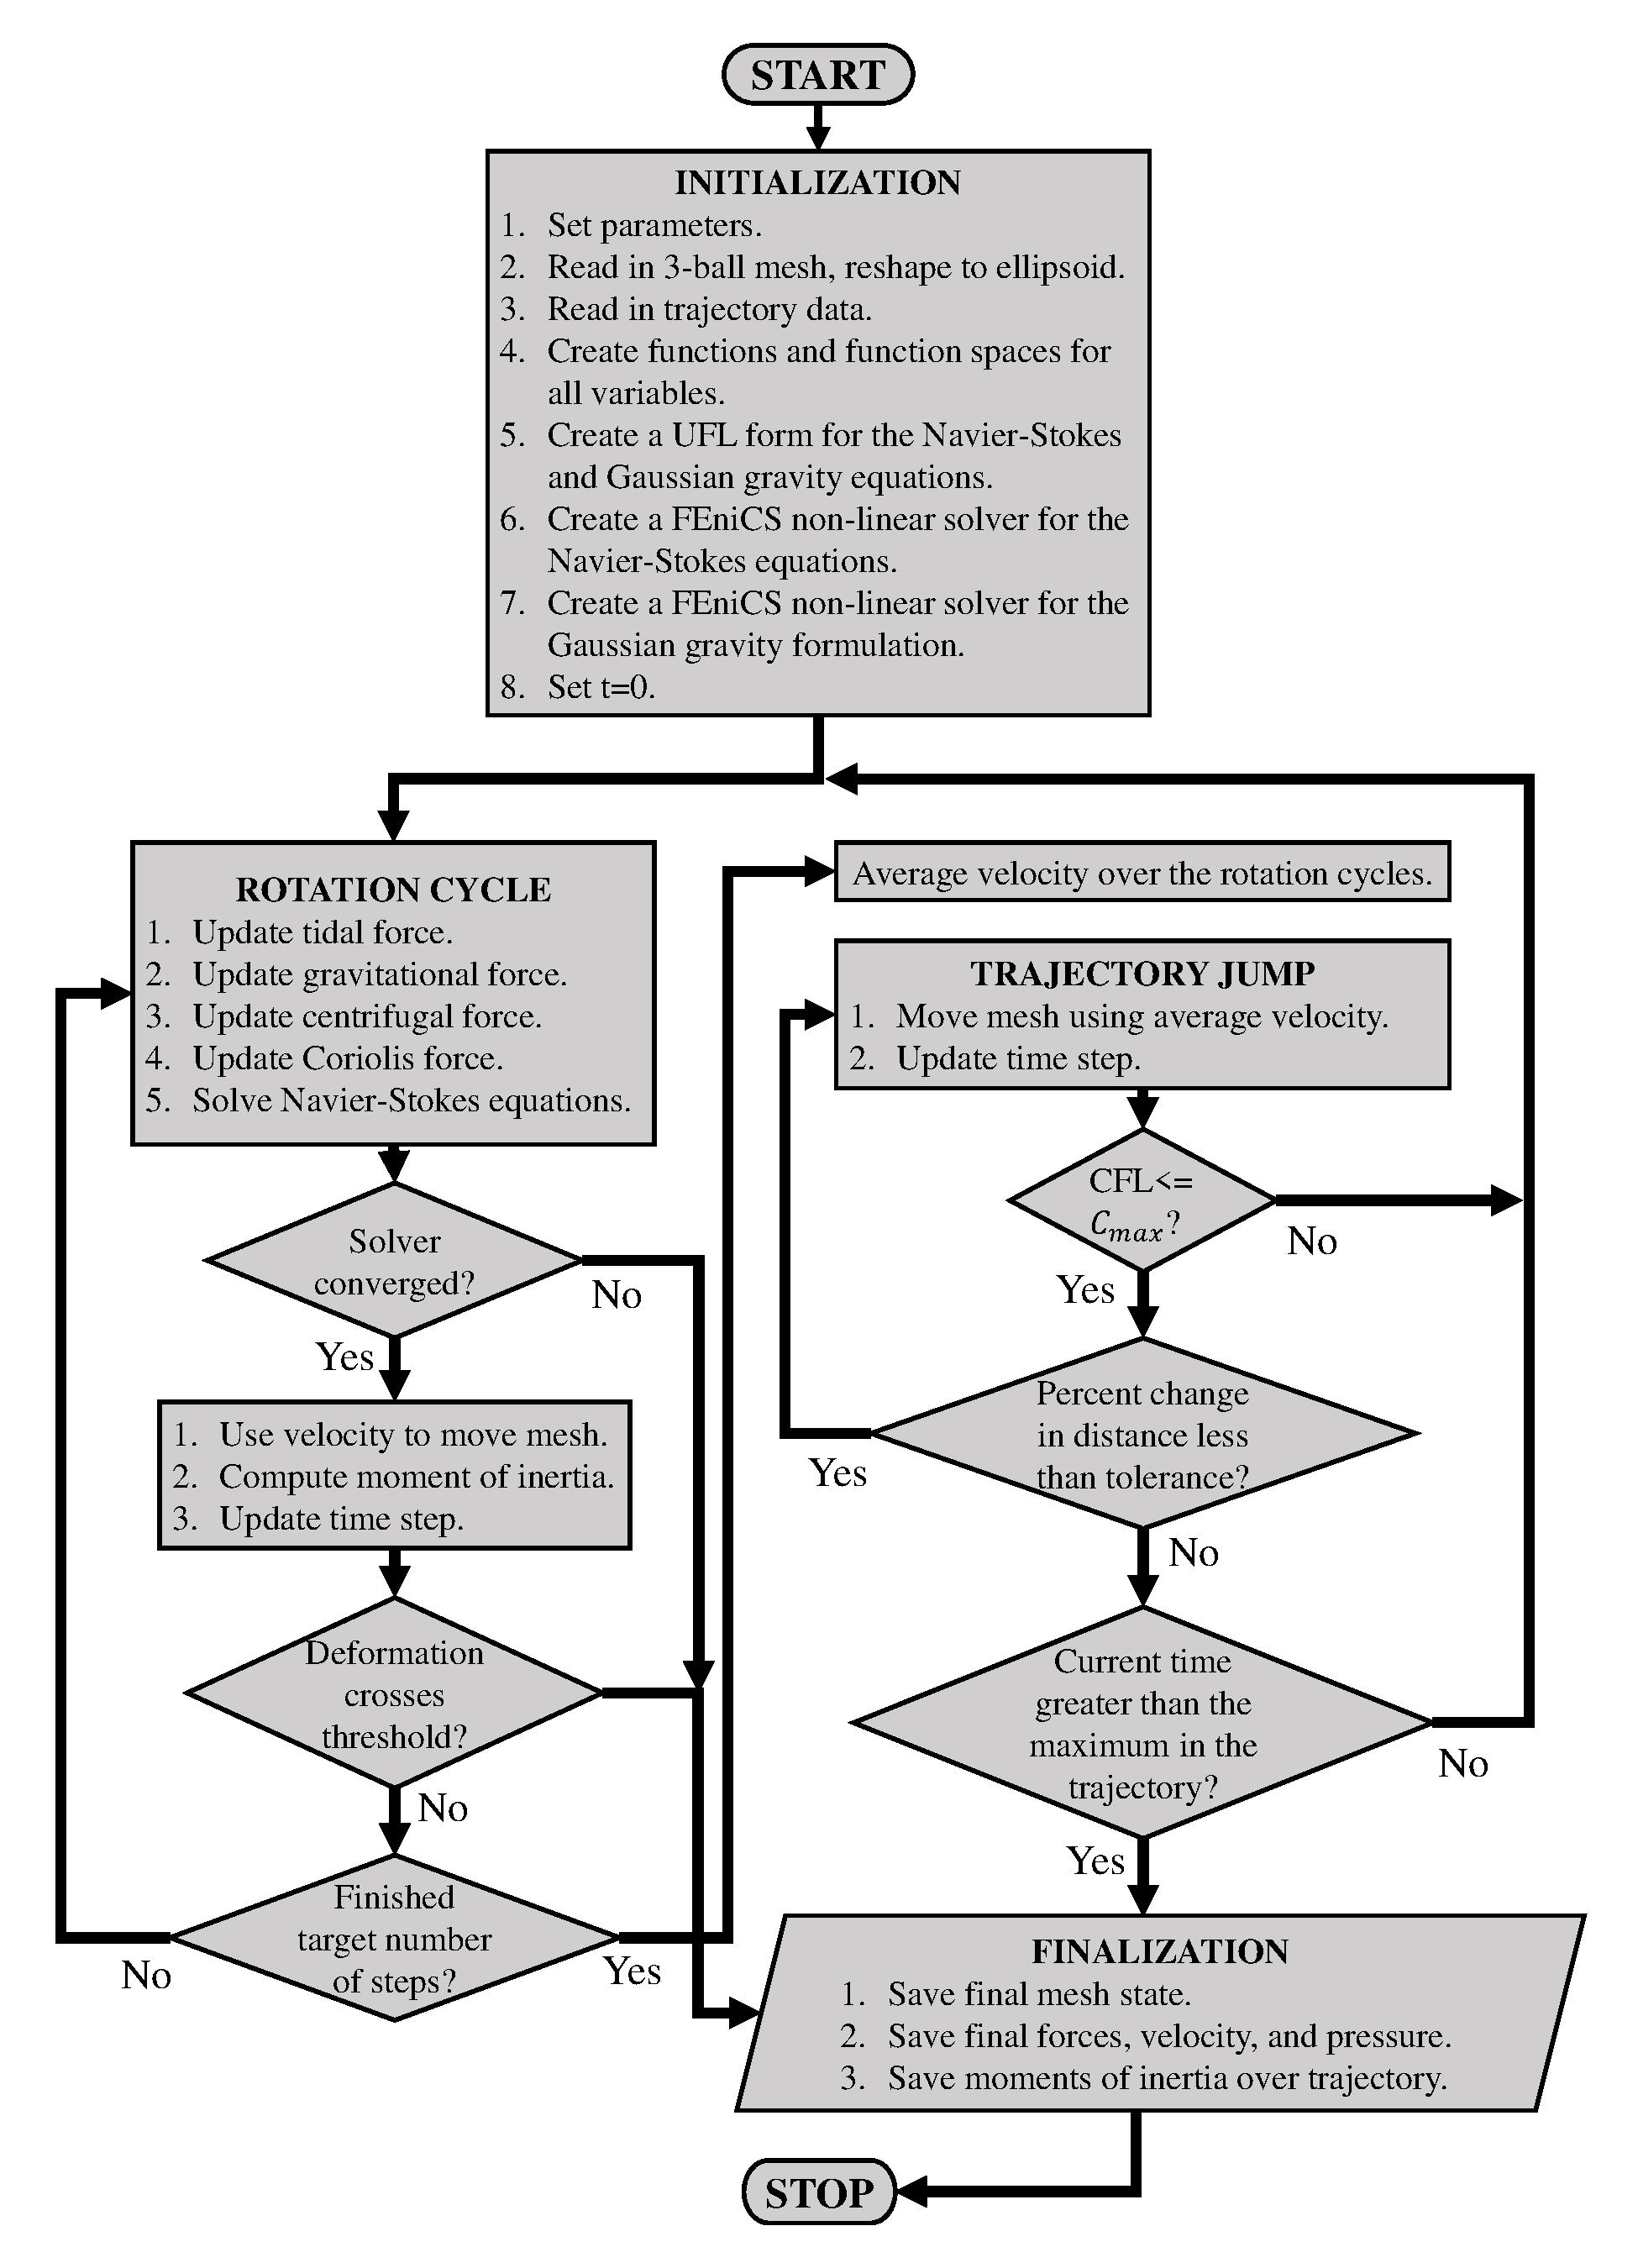
\includegraphics[width=.89\textwidth,angle=0]{SAMUSfig.pdf}
\caption{Structure of \texttt{SAMUS}.}
\label{fig:SAMUSstruct}
\end{figure*}
 
\section{Numerical Simulations of Tidal Deformation}\label{sec:numerics}

In this section, we present a generalized software, Simulator of Asteroid Malformation Under Stress (\texttt{SAMUS}), which simulates the deformation of constant-density liquid-body ellipsoids under forcing pressures, which we apply to constrain the dynamic viscosity and size of `Oumuamua. \texttt{SAMUS} incorporates tidal, centrifugal, Coriolis, and self-gravitational forces for minor bodies, and allows for customized trajectory, principal axes, rotational period, density, dynamic viscosity, rotational axis, and simulation cutoffs. It is accessible on \href{https://pypi.org/project/SAMUS/1.0.0/}{PyPi} and \href{https://github.com/astertaylor/SAMUS}{GitHub} and can be installed via \texttt{pip}.
 
\subsection{Numerical Calculations}
 
The \texttt{SAMUS} simulation software is written in Python 3.8.10 \citep{python3}, and is primarily based on the \texttt{FEniCS} \citep{fenics1,fenics2}, \texttt{UFL} \citep{UFL}, and \texttt{DOLFIN} \citep{dolfin1,dolfin2} packages. It also has dependencies on \texttt{NumPy} \citep{numpy}, \texttt{SciPy} \citep{scipy}, \texttt{pandas} \citep{pandas1,pandas2}, \texttt{quaternion} \citep{quaternion}, and \textit{MPI for Python} \citep{mpi1,mpi2,mpi3,mpi4}. All of these must be installed in the user's distribution. \texttt{SAMUS} is primarily structured as a Python class, and solves the weak formulation of the partial differential Navier-Stokes equations over a finite-element mesh.

The domain used by \texttt{SAMUS} is an $\mathcal{S}_3$ (3-ball) domain (created by Gmsh \citep{gmsh} and loaded into \texttt{DOLFIN}), distorted into an ellipsoid with principal axes $a,b,c$. After reading in the provided trajectory data, body parameters, and simulation parameters, \texttt{SAMUS} uses an Euler finite-difference approximation to iteratively solve the Navier-Stokes equations. The mesh is advectively updated at each time step to simulate the tidal deformation, where the computed fluid velocity is used to find the displacement vector. 

\texttt{FEniCS} is used to solve the weak formulation of the incompressible Navier-Stokes equations with Dirichlet boundary conditions. In the following equations, $\boldsymbol{u}=\partial\boldsymbol{r}/\partial t$ is the velocity, $\boldsymbol{r}$ is the position in the co-moving, non-inertial frame, $\rho$ is the density, $\mu$ is the dynamic viscosity, $p$ is the pressure, and $\boldsymbol{\Omega}$ is the angular velocity vector. $V$ and $Q$ are function spaces over $\mathds{R}^3$ and $\mathds{R}$ respectively,\footnote{Defined as continuous Galerkin domains.} with $\boldsymbol{u},\boldsymbol{v}\in V$ and $p,q\in Q$, and $\boldsymbol{v},q$ are test functions. The differential `$\text{d}x$' represents a volume integral over the body domain. 

The strong momentum equation is 
\begin{equation}
    \rho\frac{\partial\boldsymbol{u}}{\partial t}+\rho(\boldsymbol{u}\cdot\nabla)\boldsymbol{u}-\nabla\cdot\boldsymbol{\sigma}(\boldsymbol{u},p)=\boldsymbol{f}\,.
\end{equation}
\texttt{SAMUS} uses the weak form, which is
\begin{equation}\label{eq:momentum}
\begin{aligned}
    &\rho\frac{\partial\boldsymbol{u}}{\partial t}\cdot\boldsymbol{v}\ \text{d}x + \mu \nabla\boldsymbol{u}\cdot\nabla\boldsymbol{v}\ \text{d}x\\
    +&\rho(\boldsymbol{u}\cdot\nabla)\boldsymbol{u}\cdot\boldsymbol{v}\ \text{d}x-p\nabla\cdot\boldsymbol{v}\ \text{d}x\\
    =&\boldsymbol{F}_{\text{tidal}}\cdot\boldsymbol{v}\ \text{d}x+\boldsymbol{g}\cdot\boldsymbol{v}\ \text{d}x\\
    -&\rho (\boldsymbol{\Omega}\times(\boldsymbol{\Omega}\times\boldsymbol{r}))\cdot\boldsymbol{v}\ \text{d}x\\
    -&2\rho(\boldsymbol{\Omega}\times\boldsymbol{u})\cdot\boldsymbol{v}\ \text{d}x\ \ \ \forall\boldsymbol{v}\in V.
\end{aligned}
\end{equation}
The mass continuity equation, in its strong form, is
\begin{equation}
    \nabla\cdot\boldsymbol{u}=0,
\end{equation}
and \texttt{SAMUS} again uses the weak form,
\begin{equation}\label{eq:masscont}
    q\nabla\cdot\boldsymbol{u}\ \text{d}x=0\ \ \ \forall q\in Q.
\end{equation}

The derivation of the weak form from the strong form of the Navier-Stokes equations is given in \citet{quarteroni2014}. The right hand side of the momentum equation represents the forcing, each term of which is defined in Table \ref{table:forcing}.
 
\begin{table}[ht]
\begin{tabular}{ |l|c| } 
 \hline
 \multicolumn{2}{||c||}{FORCING TERMS} \\
 \hline\hline
 Tidal force:&$\boldsymbol{F}_{\text{tidal}} $\\ 
 \hline
 Self-gravitational force:&$\boldsymbol{g} $\\
 \hline
 Centrifugal force:&$-\rho(\boldsymbol{\Omega}\times(\boldsymbol{\Omega}\times\boldsymbol{r}))$\\
 \hline
 Coriolis force:&$-2\rho(\boldsymbol{\Omega}\times\boldsymbol{u})$.\\
 \hline
\end{tabular}

\caption{The forcing terms in the Navier-Stokes equations.}

\label{table:forcing}
\end{table}
 
In \texttt{SAMUS}, the acceleration $\partial\boldsymbol{u}/\partial t$ is estimated with an Euler finite-difference method. For a given time step indexed by $i$, the acceleration is approximated as $\partial\boldsymbol{u}/\partial t\simeq(\boldsymbol{u}_i-\boldsymbol{u}_{i-1})/\Delta t$. The time step $\Delta t$ is adaptively modified to ensure that the Courant–Friedrichs–Lewy (CFL) condition ($|\boldsymbol{u}|\Delta t/\Delta x<C_{\text{max}}$) is met \citep{CFL}. $C_{\text{max}}$ can be user-defined and is set to a default of 1, which is the standard limit. We performed extensive stability and convergence tests, which are available in the \texttt{SAMUS} package (and not described in this paper).

\texttt{SAMUS} additionally uses \texttt{FEniCS} to rapidly solve the weak form of the self-gravitational force as given by Gauss, 
\begin{equation}\label{eq:gaussgrav}
    c\nabla\cdot\boldsymbol{g}\ \text{d}x=-4\pi G\rho\ c\ \text{d}x\ \ \ \forall c\in Q\,,
\end{equation}
where $c$ is a scalar test function in $Q$. This method is relatively rapid and allows for efficient computation of self-gravity for even highly distorted bodies.
 
\texttt{SAMUS} produces a \verb|csv| file containing timestamps, the maximum size of the body on each axis, and the moment of inertia $I$ at each step, which is calculated using
\begin{equation}\label{eq:MOI}
    I=\int_S\rho\,\,\bigg(\,\frac{\|\boldsymbol{r}\times\boldsymbol{\Omega}\|^2}{\|\boldsymbol{\Omega}\|^2}\ \bigg)\, \text{d}x\,.
\end{equation}
Further, \texttt{SAMUS} is capable of incorporating a broad class of user-defined functions in these outputs.
 
 \subsection{Trajectory Jump Method}\label{subsec:trajjump}
 
\texttt{SAMUS} uses a ``trajectory jump" method for efficiency, reducing the number of computations necessary over the trajectory. \texttt{SAMUS} first computes the time-averaged deformation over a (user-defined) number of rotational periods. It then performs a linear extrapolation of this average and steps forward in simulation time until either (i) the CFL condition is violated or (ii) the heliocentric distance changes by 1\% (this threshold is similarly user-defined). This method assumes that the rotational period of the body is significantly shorter than the timescale within which the object moves through its trajectory significantly. The quality of this first-order linear approximation of the distortion was validated with convergence tests, using halved tolerances (available in the package). However, for bodies with slower rotation, further testing should be performed to confirm the validity of this methodology.
 
 \subsection{Tidal Force Computation}\label{subsec:SAMUStidalforce}
 
 In \texttt{SAMUS}, \texttt{quaternion} is used to rotate points to the stationary frame, a necessary step to compute the the continuum tidal force over $\mathcal{S}_3$. Quaternions allow for rapid computation of rotation by an arbitrary angle about an arbitrary axis, without gimbal locking \citep{kuipers2007}. For a given point $\boldsymbol{r}$ and quaternion $\boldsymbol{q}$, the rotated point is $\boldsymbol{r}'=\boldsymbol{q}\boldsymbol{r}\boldsymbol{q}^*$. A rotation by an angle $\theta$ about an axis $\boldsymbol{\hat{\Omega}}=(\Omega_x,\Omega_y,\Omega_z)$ is described by $\boldsymbol{q}=\cos{(\theta/2)}+\Omega_x\sin{(\theta/2)}\boldsymbol{i}+\Omega_y\sin{(\theta/2)}\boldsymbol{j}+\Omega_z\sin{(\theta/2)}\boldsymbol{k}$ and conjugate $\boldsymbol{q^*}=\cos{(\theta/2)}-\Omega_x\sin{(\theta/2)}\boldsymbol{i}-\Omega_y\sin{(\theta/2)}\boldsymbol{j}-\Omega_z\sin{(\theta/2)}\boldsymbol{k}$. Here, $\boldsymbol{i}$, $\boldsymbol{j}$, and $\boldsymbol{k}$ are the imaginary unit quaternions. 
 

 The position quaternion $\boldsymbol{r}'=x'\boldsymbol{i}+y'\boldsymbol{j}+z'\boldsymbol{k}$ in the co-rotating frame is given by $\boldsymbol{r}=\boldsymbol{q^*}\boldsymbol{x'}\boldsymbol{q}$ in the non-rotating frame. The tidal force at each point on the body is then computed by \texttt{SAMUS} using 
\begin{equation}\label{eq:samustide}
    \boldsymbol{F}_{\text{tidal}}(\boldsymbol{r}')=-\boldsymbol{\hat{x}}GM_{\Sun}\rho\left(\frac{1}{(r_H-(\boldsymbol{q^*}\boldsymbol{r}'\boldsymbol{q})_x)^2}-\frac{1}{r_H^2}\right)\,,
\end{equation}
for an object with constant density $\rho$. 
 
\subsection{Pseudocode}
 
In this subsection we present a pseudocode which demonstrates the most basic functionality of \texttt{SAMUS}. As a class method, \texttt{SAMUS} is capable of running in a modular format with complex function call patterns. In steps 1-8, we initialize the simulation. In steps 9.a-9.d, we compute the forcing functions described in \S\ref{subsec:SAMUStidalforce}, Table \ref{table:forcing}, and Equation \ref{eq:gaussgrav}. In steps 9.e-9.i, we update the model for a single time step. In steps 10 and 11, we implement the trajectory jump method described in \S\ref{subsec:trajjump}, and in step 12, we save and output simulation products. A script to replicate this example is available in the \texttt{SAMUS} package. 

\begin{enumerate}
\itemsep0em
    \item[]\texttt{SAMUS Pseudocode}
    \item\texttt{Set parameters. }
    \item\texttt{Read in 3-ball mesh and reshape to ellipsoid.}
    \item\texttt{Read in trajectory data.}
    \item\texttt{Create functions and function spaces for all variables.}
    \item\texttt{Create a UFL form for the Navier-Stokes equations.}
    \item\texttt{Create a FEniCS non-linear solver for the Navier-Stokes equations.}
    \item\texttt{Create a FEniCS non-linear solver for the Gaussian gravity formulation.}
    \item\texttt{Set t=0.}
    \item\begin{description}
            \item[WHILE]\verb|Number of cycles < number in loop:|
            \begin{enumerate}
                \item\texttt{Update tidal force, computed using Eqn }\ref{eq:samustide}.
                \item\texttt{Update gravitational force, computed using Eqn }\ref{eq:gaussgrav}.
                \item\texttt{Update Coriolis force, computed using the relevant term from Table }\ref{table:forcing}.
                \item\texttt{Update centrifugal force, computed using the relevant term from Table }\ref{table:forcing}.
                \item\texttt{Solve Navier-Stokes equations. If this diverges, STOP.}
		\item\texttt{Move mesh with velocity.}
                \item\texttt{Check if deformation crosses threshold. If it does, STOP.}
		\item\texttt{Compute moment of inertia using Equation \ref{eq:MOI}.}
		\item\texttt{Update time step.}
            \end{enumerate}
	\end{description}
    \item\texttt{Average velocities over the rotation cycles.}
    \item\begin{description}
            \item[WHILE]\texttt{Change in the heliocentric distance is less than tolerance:}
            \begin{enumerate}
                \item\texttt{Check to ensure that CFL<C}$_{\texttt{max}}$.
                \item\texttt{Move mesh using average velocity}.
                \item\texttt{Update time step.}
            \end{enumerate}
	\end{description}
    \item[\textbf{IF}:]\texttt{The number of steps is less than the upper limit, then repeat Steps 8-11.}
    \item\texttt{Save the mesh, the functions, and the moments of inertia over the path.}
\end{enumerate}

This pseudocode structure is also shown in Figure \ref{fig:SAMUSstruct}.

\begin{figure}
\centering
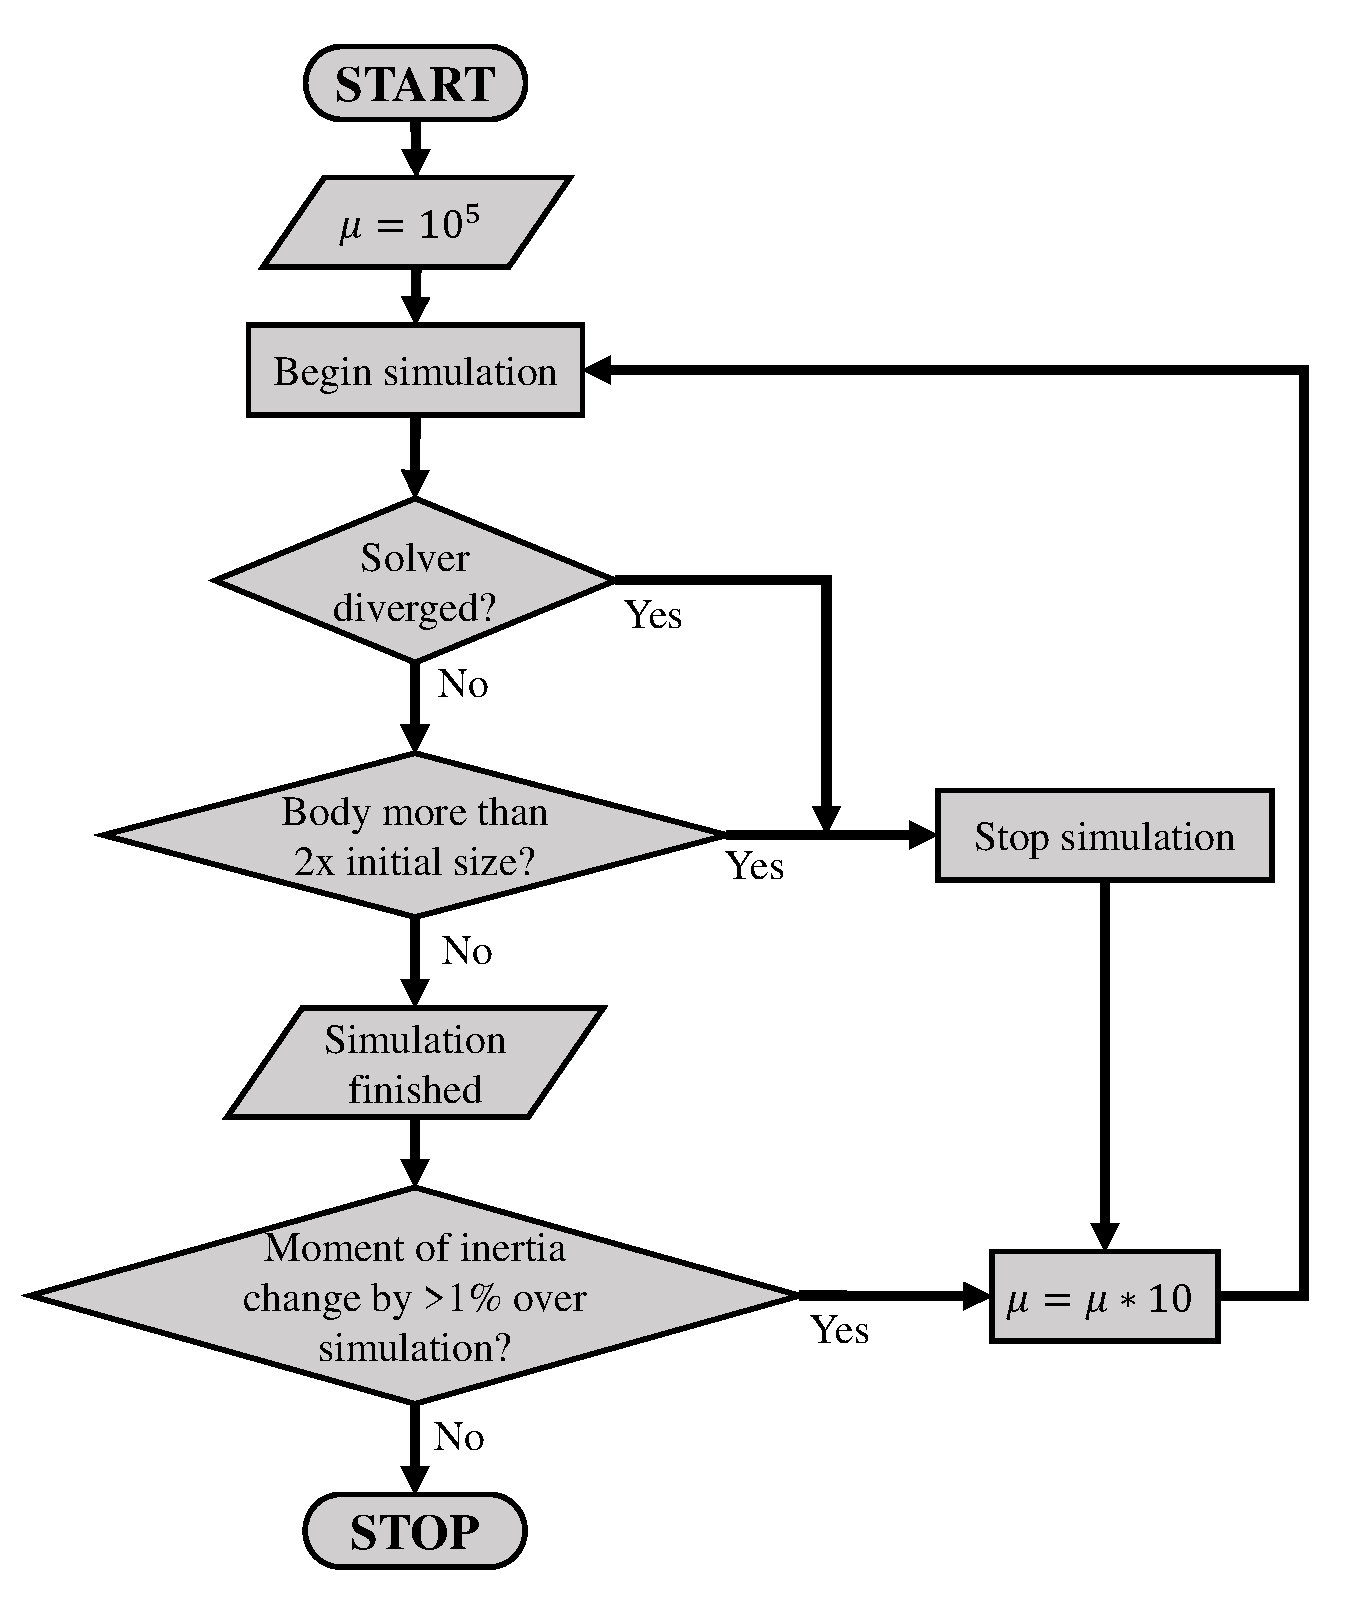
\includegraphics[width=\linewidth,angle=0]{simflowchart.pdf}
\caption{Flowchart showing the structure of the simulation runs used to model `Oumuamua.}
\label{fig:simstruct}
\end{figure}
\begin{figure}
\centering
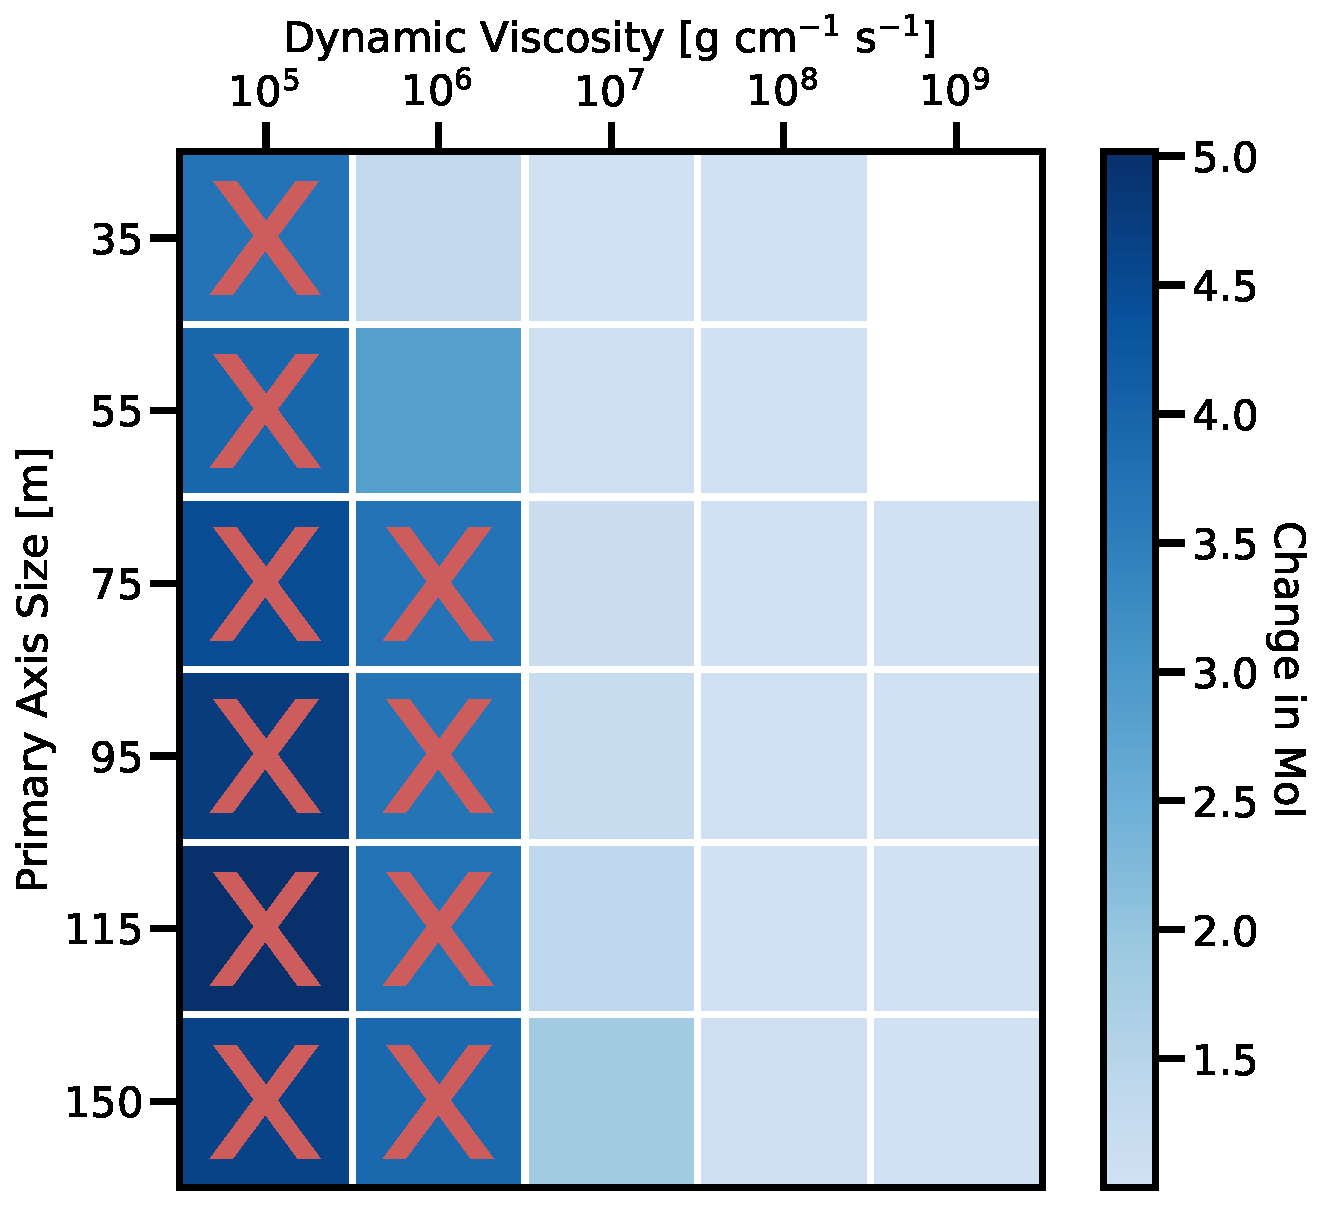
\includegraphics[width=\linewidth,angle=0]{optimal_axis_heatmap.pdf}
\caption{Simulated change of `Oumuamua's moment of inertia from 2017 May 4 to 2018 January 16. Red X's indicate simulations that were halted because of disintegration or numerical divergence. Empty squares indicate parameters for simulations that were not run, as convergence was achieved for lower dynamic viscosity values. }
\label{fig:optimalaxisheatmap}
\end{figure}

\section{`Oumuamua Simulation}\label{sec:oumuamuasim}

In this section, we implement \texttt{SAMUS} to constrain the size and dynamic viscosity of `Oumuamua. We adopt axes of 6:6:1 and a bulk density of $\rho=0.5$ g cm$^{-3}$, which is typical for Solar System comets \citep{britt2006}. We run simulations with an initial primary axis of $a=35,55,75,95,115$, and 150 meters in diameter, using the optimal single-axis rotation described in \S\ref{subsec:gettingaxis}. The rotation axis is $\boldsymbol{\hat{\Omega}}=0.1509\boldsymbol{\hat{x}}+0.3075\boldsymbol{\hat{y}}+0.9395\boldsymbol{\hat{z}}$, and we assume a constant rotational period of $p=7.3975$ hours. While these are held constant in each simulation, the simulated body undergoes significant deformation which produces a change in the spin period, assuming conservation of angular momentum. The simulations are run from 2017 May 4 to 2018 January 16, using trajectory data obtained from the \href{https://ssd.jpl.nasa.gov/horizons.cgi}{JPL Horizons database}.

We also ran simulations with rotations about each principal axis, and verified that this does not significantly affect the results, validating our use of the optimal rotation axis. These simulations are not shown. 

We initialize each simulation with a dynamic viscosity of $\mu=10^5$ g cm$^{-1}$ s$^{1}$, approximately equal to that of peanut butter under high pressure \citep{citerne2001}. The simulation is halted if the body is distorted to more than twice its initial size, as the cometary materials should disintegrate with such significant force, although shear tolerances are unknown. The simulation is reset and the viscosity increased by an order of magnitude if (i) the solvers for the Navier-Stokes equations fail to converge or (ii) the moment of inertia changes by more than 1\% over the path. These simulations are run with a trajectory jump tolerance of 1\% (see \S \ref{subsec:trajjump}), and $C_{\text{max}}=1$. We compute 10 time steps over each rotational period, which fully samples the force over the rotation. For clarity, a flowchart describing this structure is shown in Figure \ref{fig:simstruct}, and the code used to create these simulations is available on \href{https://github.com/astertaylor/Oumuamua}{GitHub}.

\begin{figure}
\centering
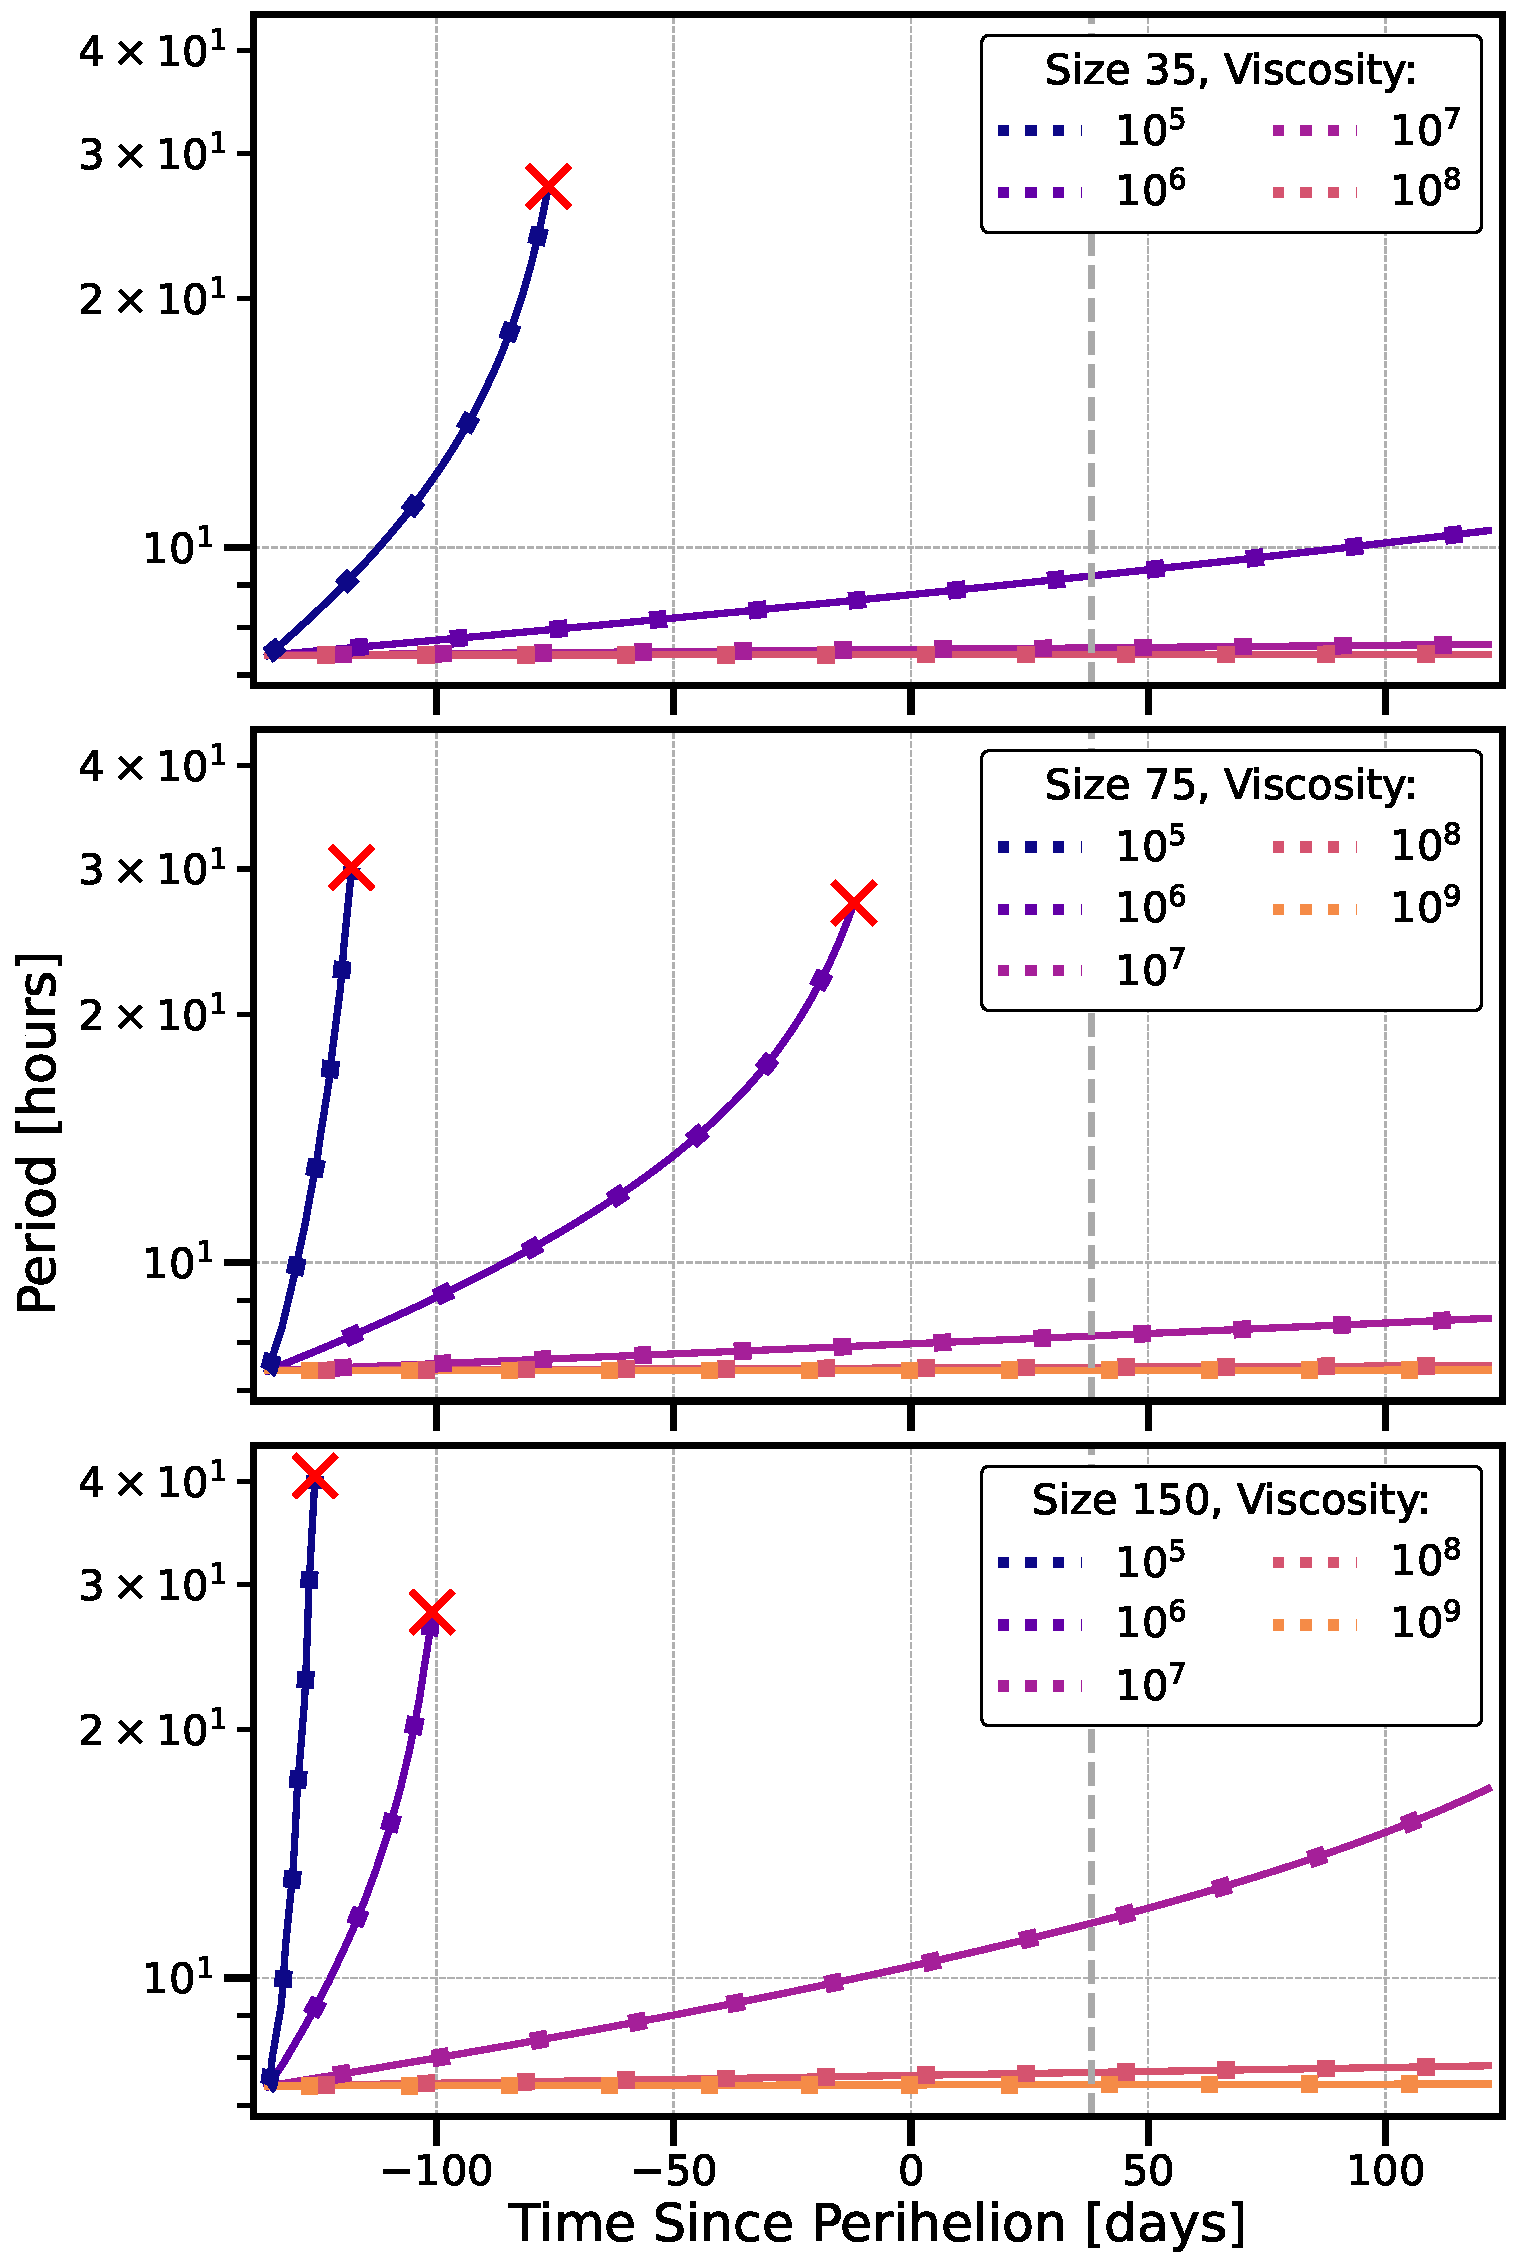
\includegraphics[width=\linewidth,angle=0]{optimal_axis_periods.pdf}
\caption{Evolution of `Oumuamua's spin period due to modulation in the moment of inertia. The period is initialized at $p=7.3906$, ensuring that $p=7.3975$ hours at discovery (vertical dashed line) for the optimal fit. Rows represent different initial sizes. }
\label{fig:optimalaxisperiods}
\end{figure}

\begin{figure*}
\centering
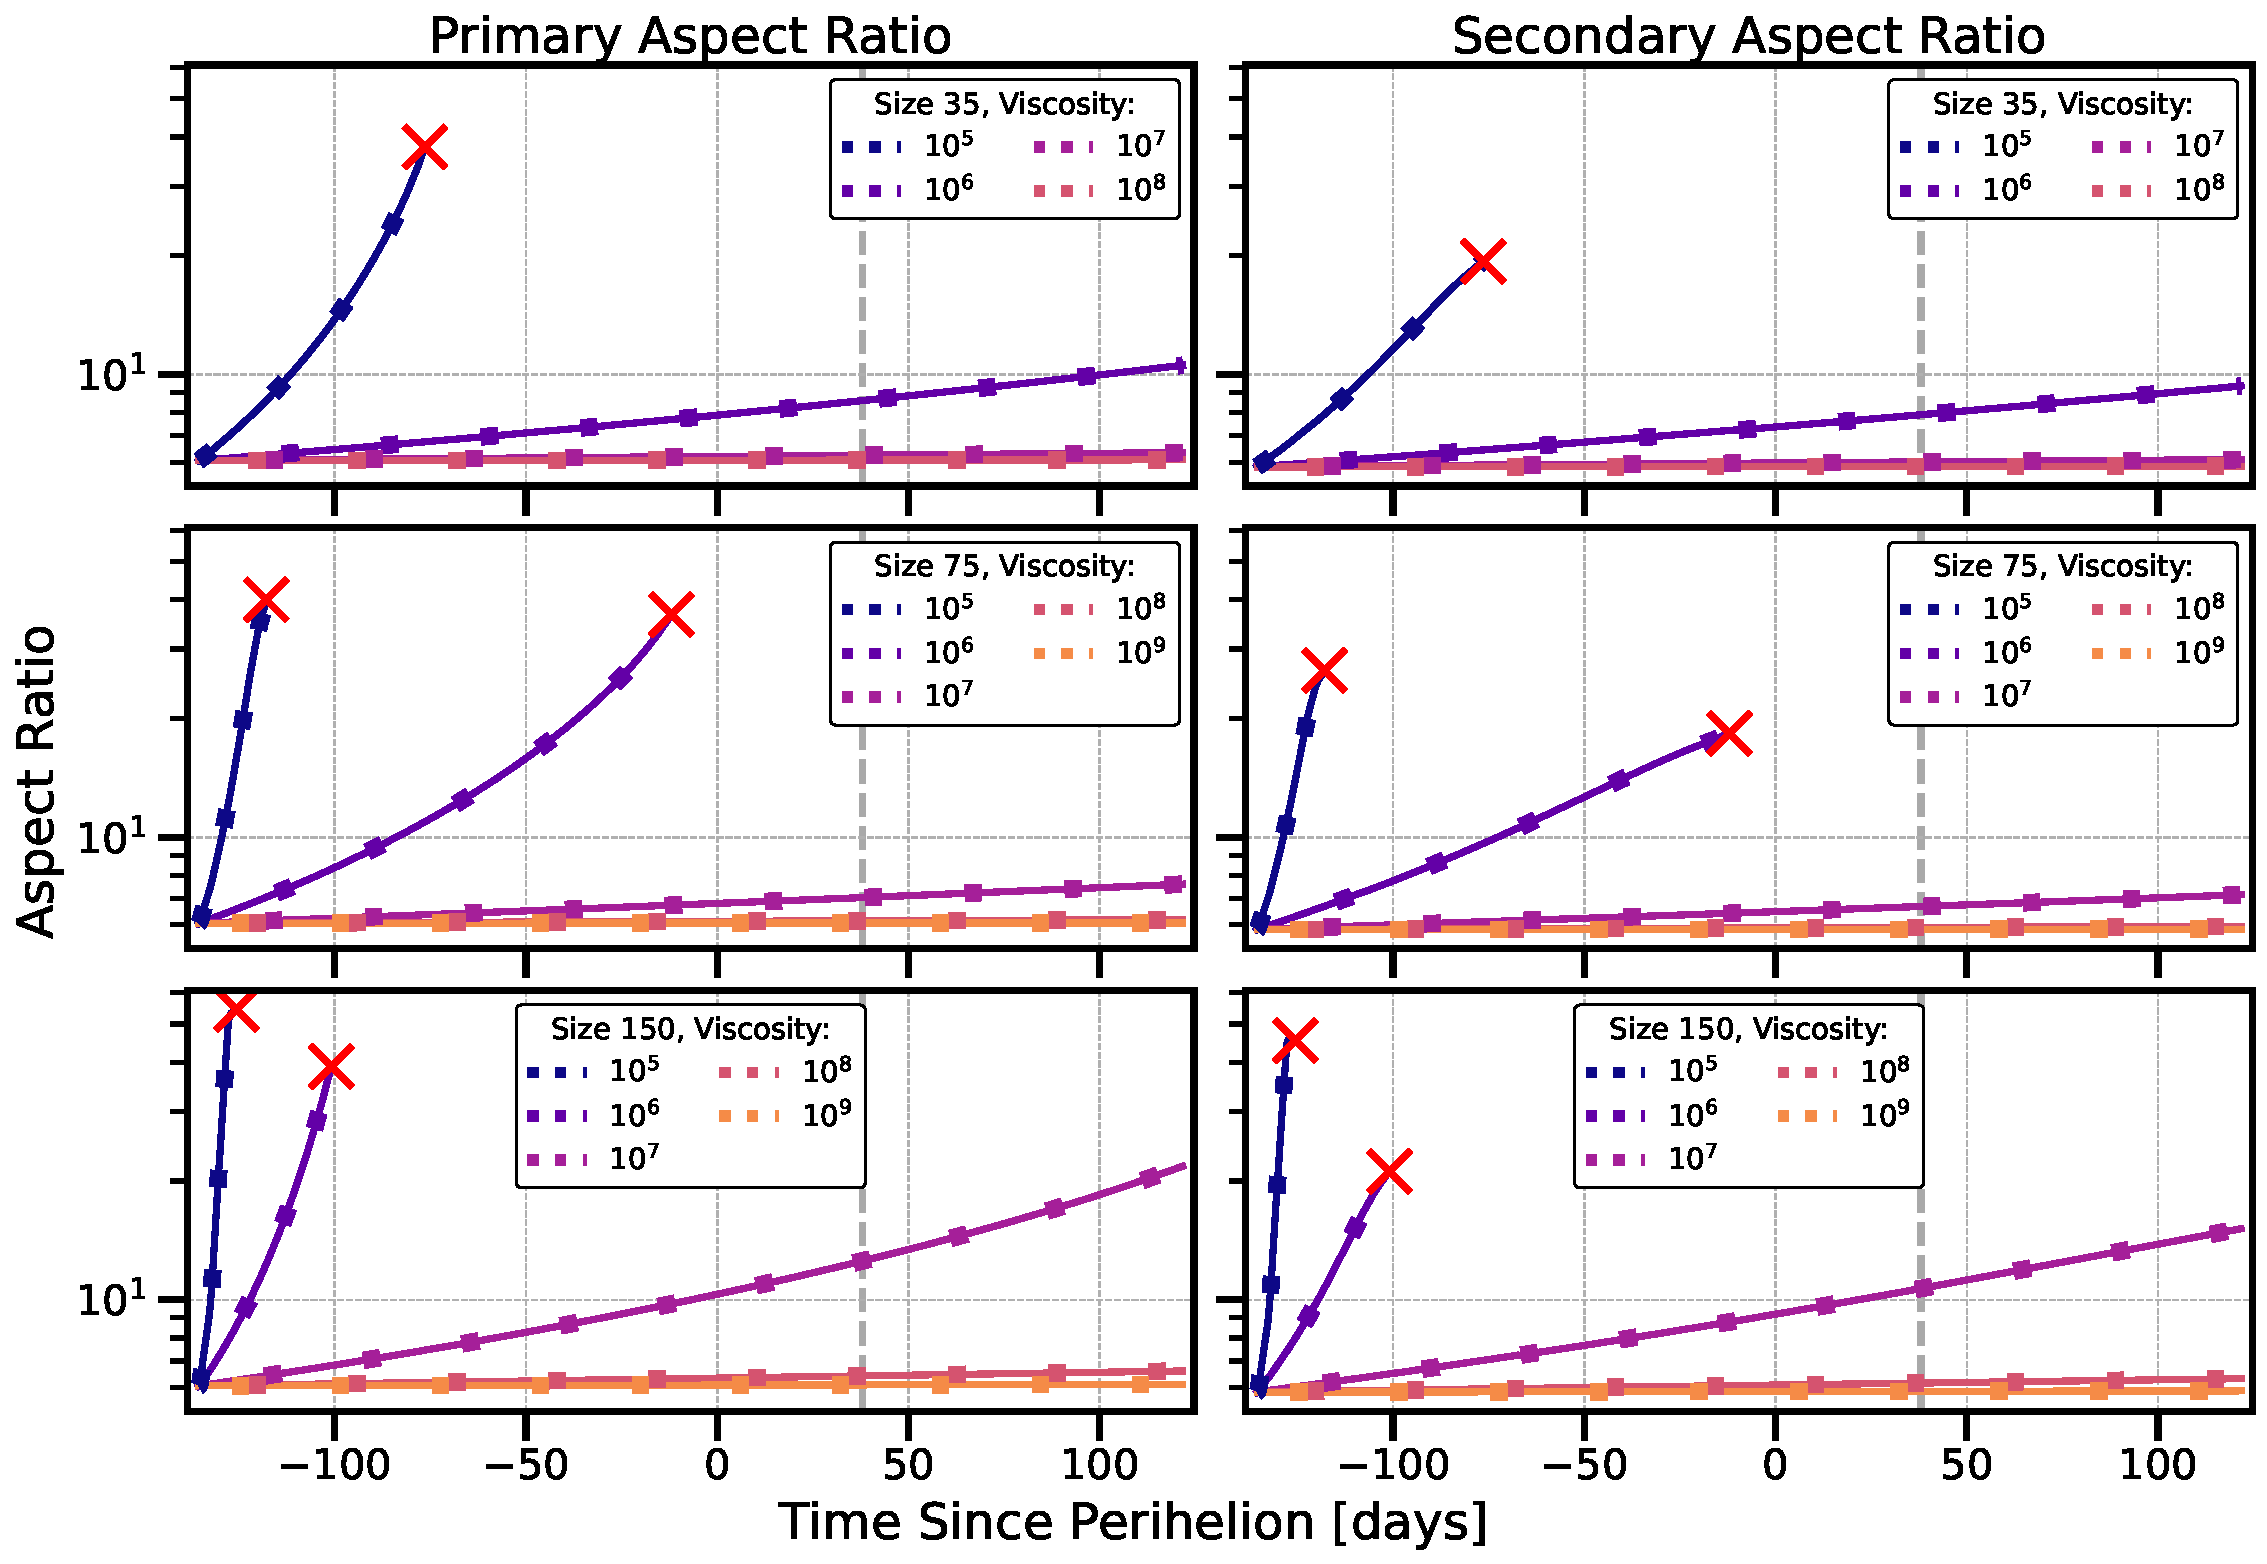
\includegraphics[width=\linewidth,angle=0]{optimal_axis_aspect_ratio.pdf}
\caption{Evolution of `Oumuamua's aspect ratios due to tidal deformation. The primary aspect ratio (left column) is the ratio of the largest to the smallest axis, while the secondary (right column) is the ratio of the intermediate to the smallest axis. At $t=0$, both aspect ratios are 6. The time of discovery is plotted as a vertical dashed line.}
\label{fig:optimalaxisaspectratio}
\end{figure*}

\begin{figure*}
\centering
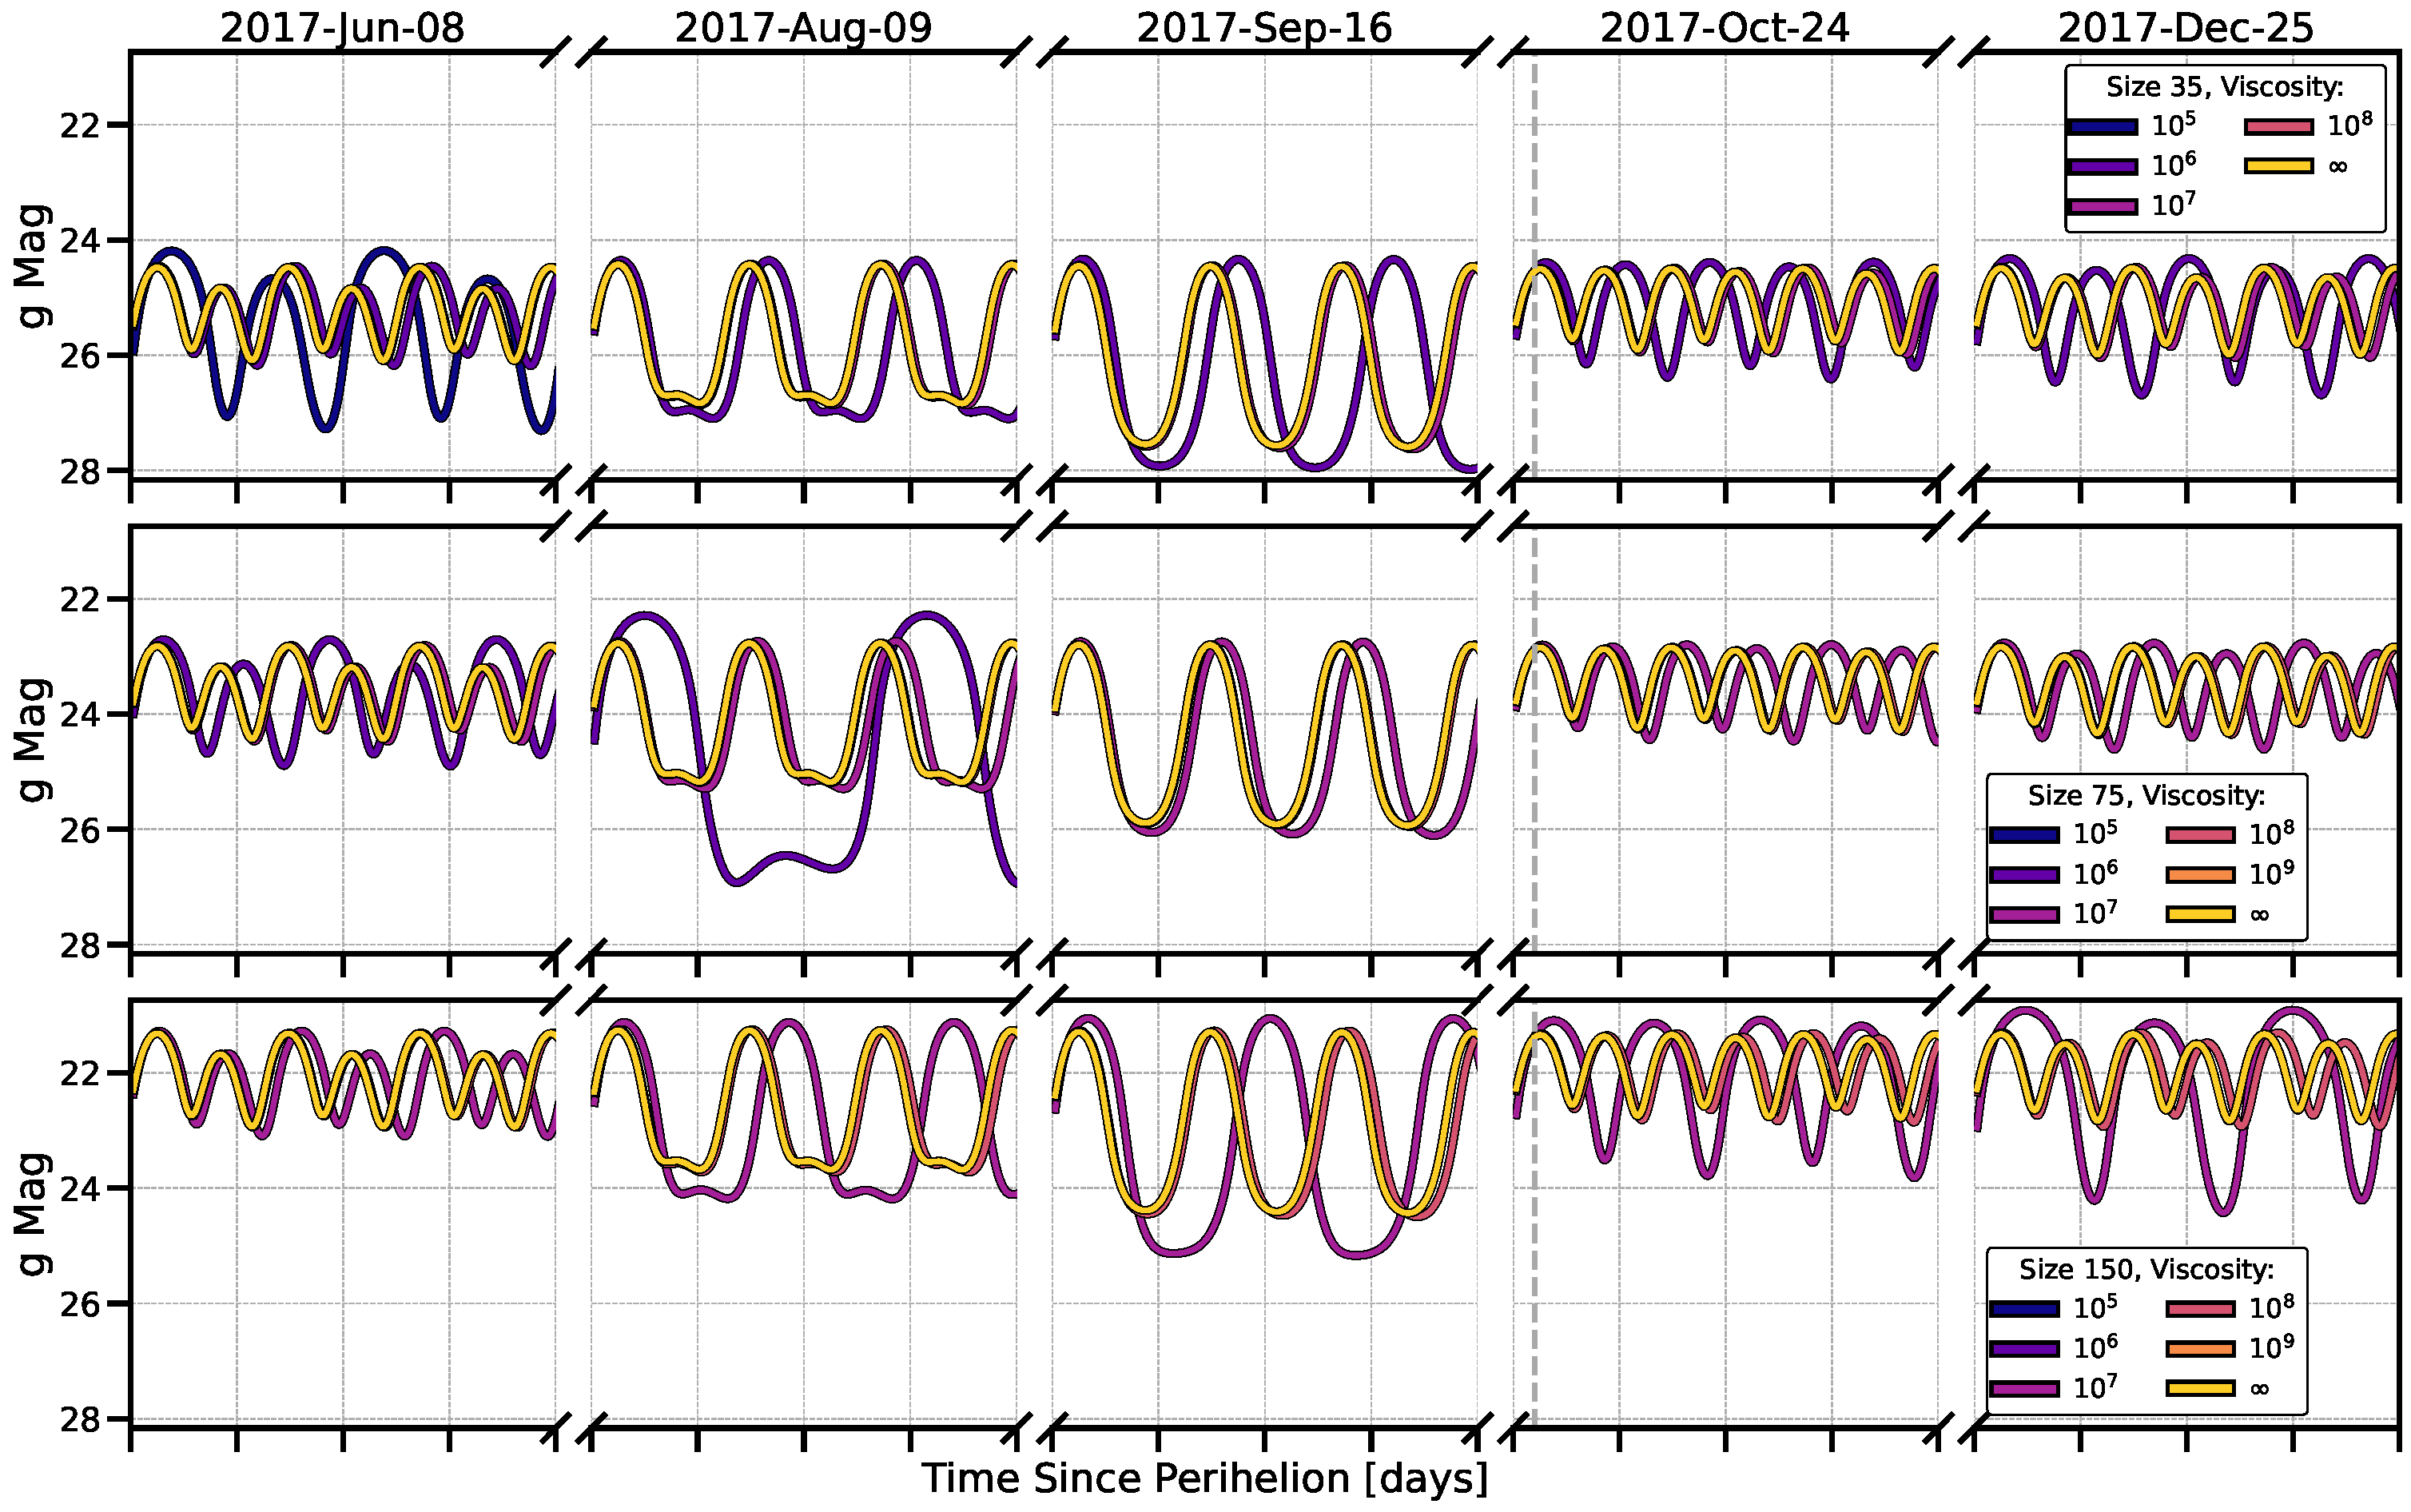
\includegraphics[width=\linewidth,angle=0]{optimal_axis_lightcurve_sims.pdf}
\caption{Synthetic light curves of `Oumuamua which incorporate simulated changes in period and aspect ratio from tidal deformation. Rows correspond to the initial sizes and colors correspond to the dynamic viscosities of the body in the simulations. The time of discovery is indicated with a vertical dashed line.}
\label{fig:optimalaxislightcurvesims}
\end{figure*}

In Figure \ref{fig:optimalaxisheatmap}, we present an overview of all of the simulations. The moment of inertia is calculated as $I(t)=\int\rho \boldsymbol{r}(t)^2\text{d}x$, and we show $I(t_\text{max})/I(0)$. These changes in the moment of inertia will also affect the spin period. 

To quantify this effect, we assume an idealized scenario in which the spin period only changes in response to tidal deformation and subsequent changes in the moment of inertia. This is not realistic, because outgassing torques should dominate the rotational state. We assume that the angular momentum is conserved such that $L(0)=L(t)$, where $L(t)=I(t) \omega(t)$ and $\omega(t)$ is the angular frequency. We additionally set $p(0)=7.3906$ hours, chosen such that the object has $p=7.3975$ hours at the time of detection, for the simulation which produced an optimal fit to the photometric data. The evolution of the spin period is shown in Figure \ref{fig:optimalaxisperiods} and the aspect ratios in Figure \ref{fig:optimalaxisaspectratio}. For high viscosities, the aspect ratios and the spin period are approximately constant, as the viscous forces are much stronger than the deformation forces. The rotational period increases in every case, since tidal deformation only increases the moment of inertia. Therefore, this effect cannot explain the spin-up detected in the photometric data between October and November. However, it could contribute to the October spin-down reported by \citet{flekkoy2019}. Although these simulations are highly idealized and do not incorporate outgassing torques, it is clear that tidal deformation can change the rotational state and light curve amplitude. 

\begin{table*}[t]
\begin{tabular}{ |c||c|c|c|c|c|c| } 
 \hline
 \multicolumn{7}{||c||}{$\chi^2$ of SIMULATED LIGHT CURVES vs DATA} \\
 \hline\hline
 \multicolumn{1}{|c}{Size [m]} & \multicolumn{6}{|c|}{Dynamic Viscosity [g cm$^{-1}$ s$^{-1}$]} \\
 \hline\hline
 \multicolumn{1}{|c||}{} & $10^5$ & $10^6$ & $10^7$ & $10^8$ & $10^9$ & $\infty$ \\
 \hline\hline
 35 & - & 5.038e+04 & 3.882e+04 & 3.833e+04 & - & 3.831e+04 \\
 \hline
 55 & - & 1.078e+05 & 3.981e+04 & 3.840e+04 & - & 3.835e+04 \\
\hline
75 & - & - & 4.175e+04 & 3.851e+04 & 3.830e+04 & 3.829e+04 \\
\hline
95 & - & - & 4.539e+04 & 3.867e+04 & 3.832e+04 & 3.830e+04 \\
\hline
115 & - & - & 5.217e+04 & 3.886e+04 & 3.833e+04 & 3.831e+04 \\
\hline
150 & - & - & 8.213e+04 & 3.935e+04 & 3.837e+04 & 3.833e+04 \\
\hline
\end{tabular}
\caption{ $\chi^2$ values for each synthetic light curve fit to the photometric data. '-'s indicate simulations which were numerically unstable.}
\label{table:simdatachi2}
\end{table*}

Overall, objects with larger sizes undergo significantly more deformation and require larger viscosities to maintain stability. A dynamic viscosity of $\mu=10^7$ g cm$^{-1}$ s$^{-1}$ is sufficient for all sizes to be non-divergent over the trajectory. For initial sizes of 35 and 55 meters, $\mu=10^8$ g cm$^{-1}$ s$^{-1}$ lead to only small-scale changes in the body over its trajectory. For the remaining sizes (75, 95, 115, and 150 meters), $\mu=10^9$ g cm$^{-1}$ s$^{-1}$ similarly allows only minor changes. 

\section{Synthetic Light Curves Incorporating Tidal Effects}\label{sec:lightcurvesim}

In this section, we present synthetic light curves for `Oumuamua over 5 1-day periods which incorporate the effects of tidal deformation. These 5 1-day periods begin on 2017 May 4, 2017 August 9, 2017 September 15 (perihelion), 2017 October 24 (detection), and 2018 January 29 (final simulated point). As before, trajectory and phase angle data are obtained from \href{https://ssd.jpl.nasa.gov/horizons.cgi}{JPL's Horizons database}. 

The light curves are computed with Equation \ref{eq:MLmodel} (the ML15 model) assuming optimal axis parameters (\S \ref{subsec:gettingaxis}). The ML15 model incorporates a Lommel-Seeliger scattering surface for an ellipsoidal body, phase angle effects, and an arbitrary orientation and rotation. We compute the period evolution using the time evolution of the aspect ratio and moment of inertia (Figures \ref{fig:optimalaxisperiods} and \ref{fig:optimalaxisaspectratio}) computed in \S\ref{sec:oumuamuasim}. This period is used to compute the orientation, $\beta$, as $\beta=2\pi\,(t\%p)/p$. The ML15 model also incorporates the instantaneous aspect ratio into the light curve. The final synthetic light curves that incorporate amplitude and period modulations are presented in Figure \ref{fig:optimalaxislightcurvesims}. For comparison, we also show light curves with constant period and aspect ratio, which correspond to the dynamic viscosity $\mu\rightarrow\infty$.

Each model is initialized on 2017 May 4 with period $p=7.3975$ and aspect ratio 6:6:1. The parameters for the observation vector and the rotation axis are the optimal results from \S\ref{subsec:gettingaxis}. As these simulations use initial sizes which were obtained from data measured in October 2017, these light curves do not match up well with available photometric data, but instead provide qualitative examples of an evolving light curve due to tidal effects. 

These light curves are corrected for brightness variation due to the object's helio- and geo-centric distances. Therefore, amplitude variations are due to modulations of the aspect ratio and/or phase angle. Larger objects have brighter average magnitudes because the albedo is constant in all simulations. There are curious features in the light curves in August, which are due to changes in phase angle (\S \ref{subsec:phaseaspectanalysis}). 

Aside from the effects of phase angle and period modulations, there is little variation in the shape of these light curves. Additionally, there is a notable decrease in amplitude post-perihelion. While the aspect ratio does increase during this time period, this feature in the light curve is entirely due to the phase angle. This effect is most obvious for the low-viscosity simulations. This implies that the evolving aspect ratio does not produce an observable signature in the amplitude for these simulation parameters. While tidal deformation can significantly alter the spin period, its effect on the amplitude of the light curve is not detectable for `Oumuamua. Period and amplitude changes in light curves of future interstellar objects may result from tidal deformation, and could be used to constrain the material composition. 

\begin{figure}[ht]
\centering
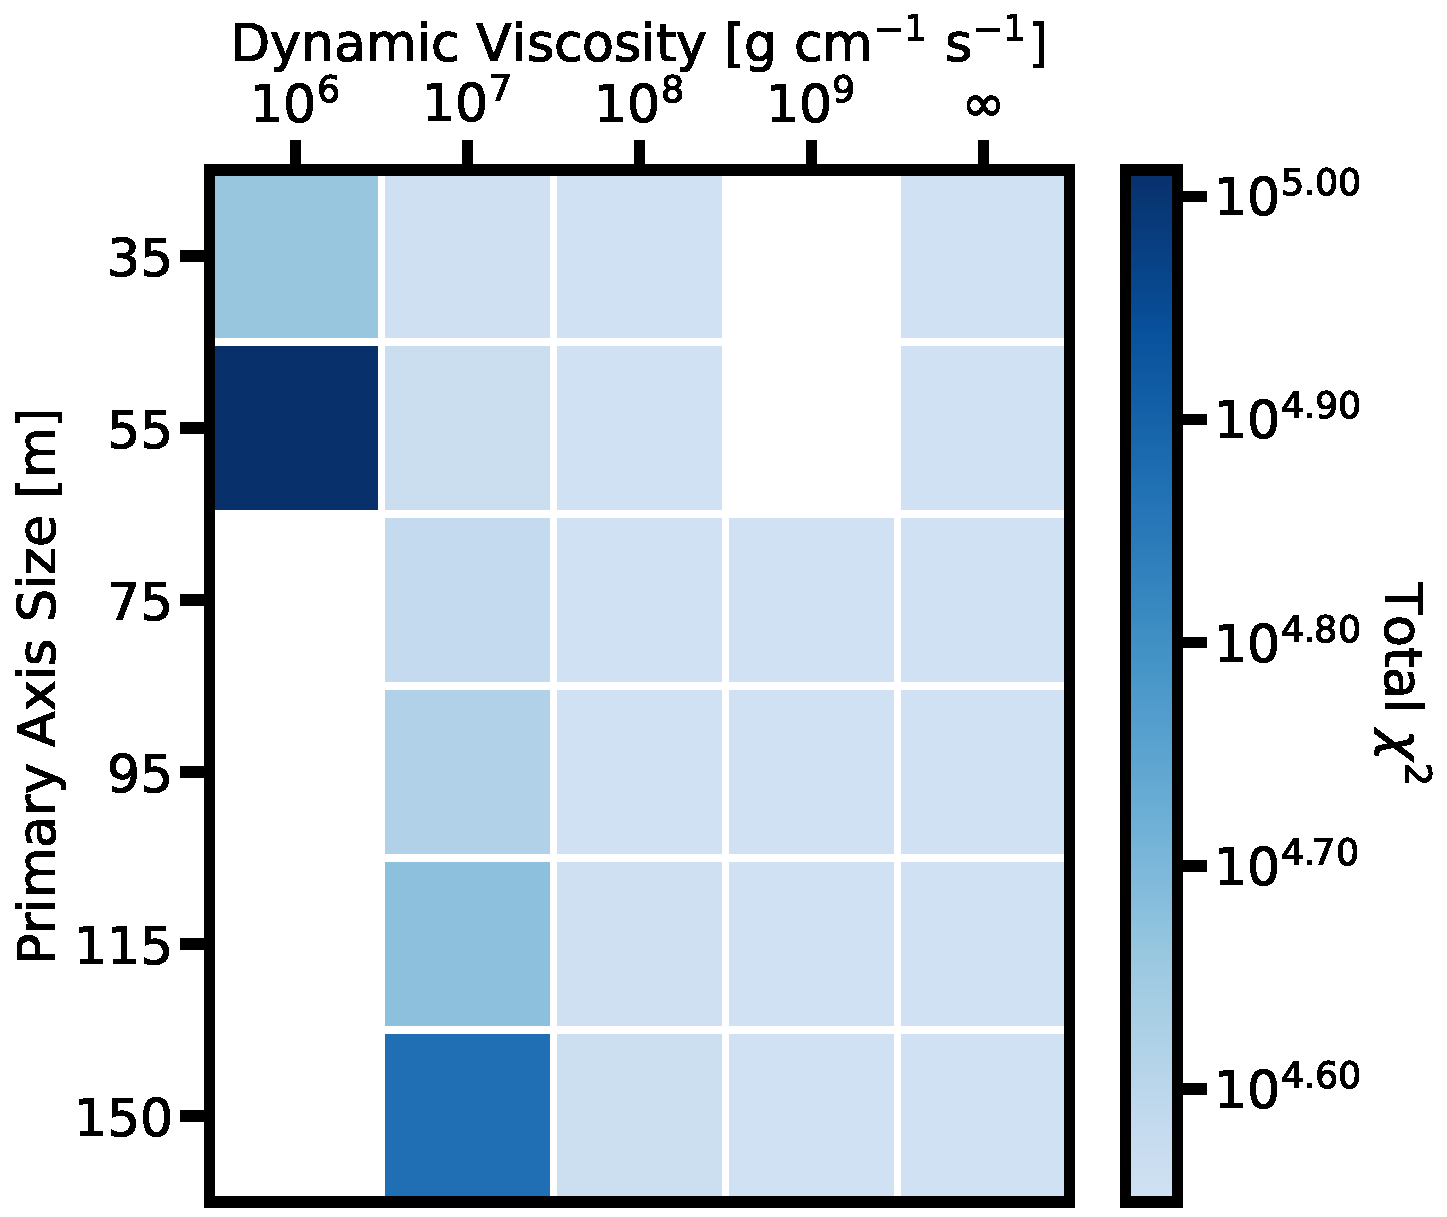
\includegraphics[width=.98\linewidth,angle=0]{sim_chi2_heatmap.pdf}
\caption{Best fit $\chi^2$ values between synthetic and photometric data. Empty spaces indicate parameter choices for simulations that were not run.}
\label{fig:simdatachi2heatmap}
\end{figure}

\begin{figure*}
\centering
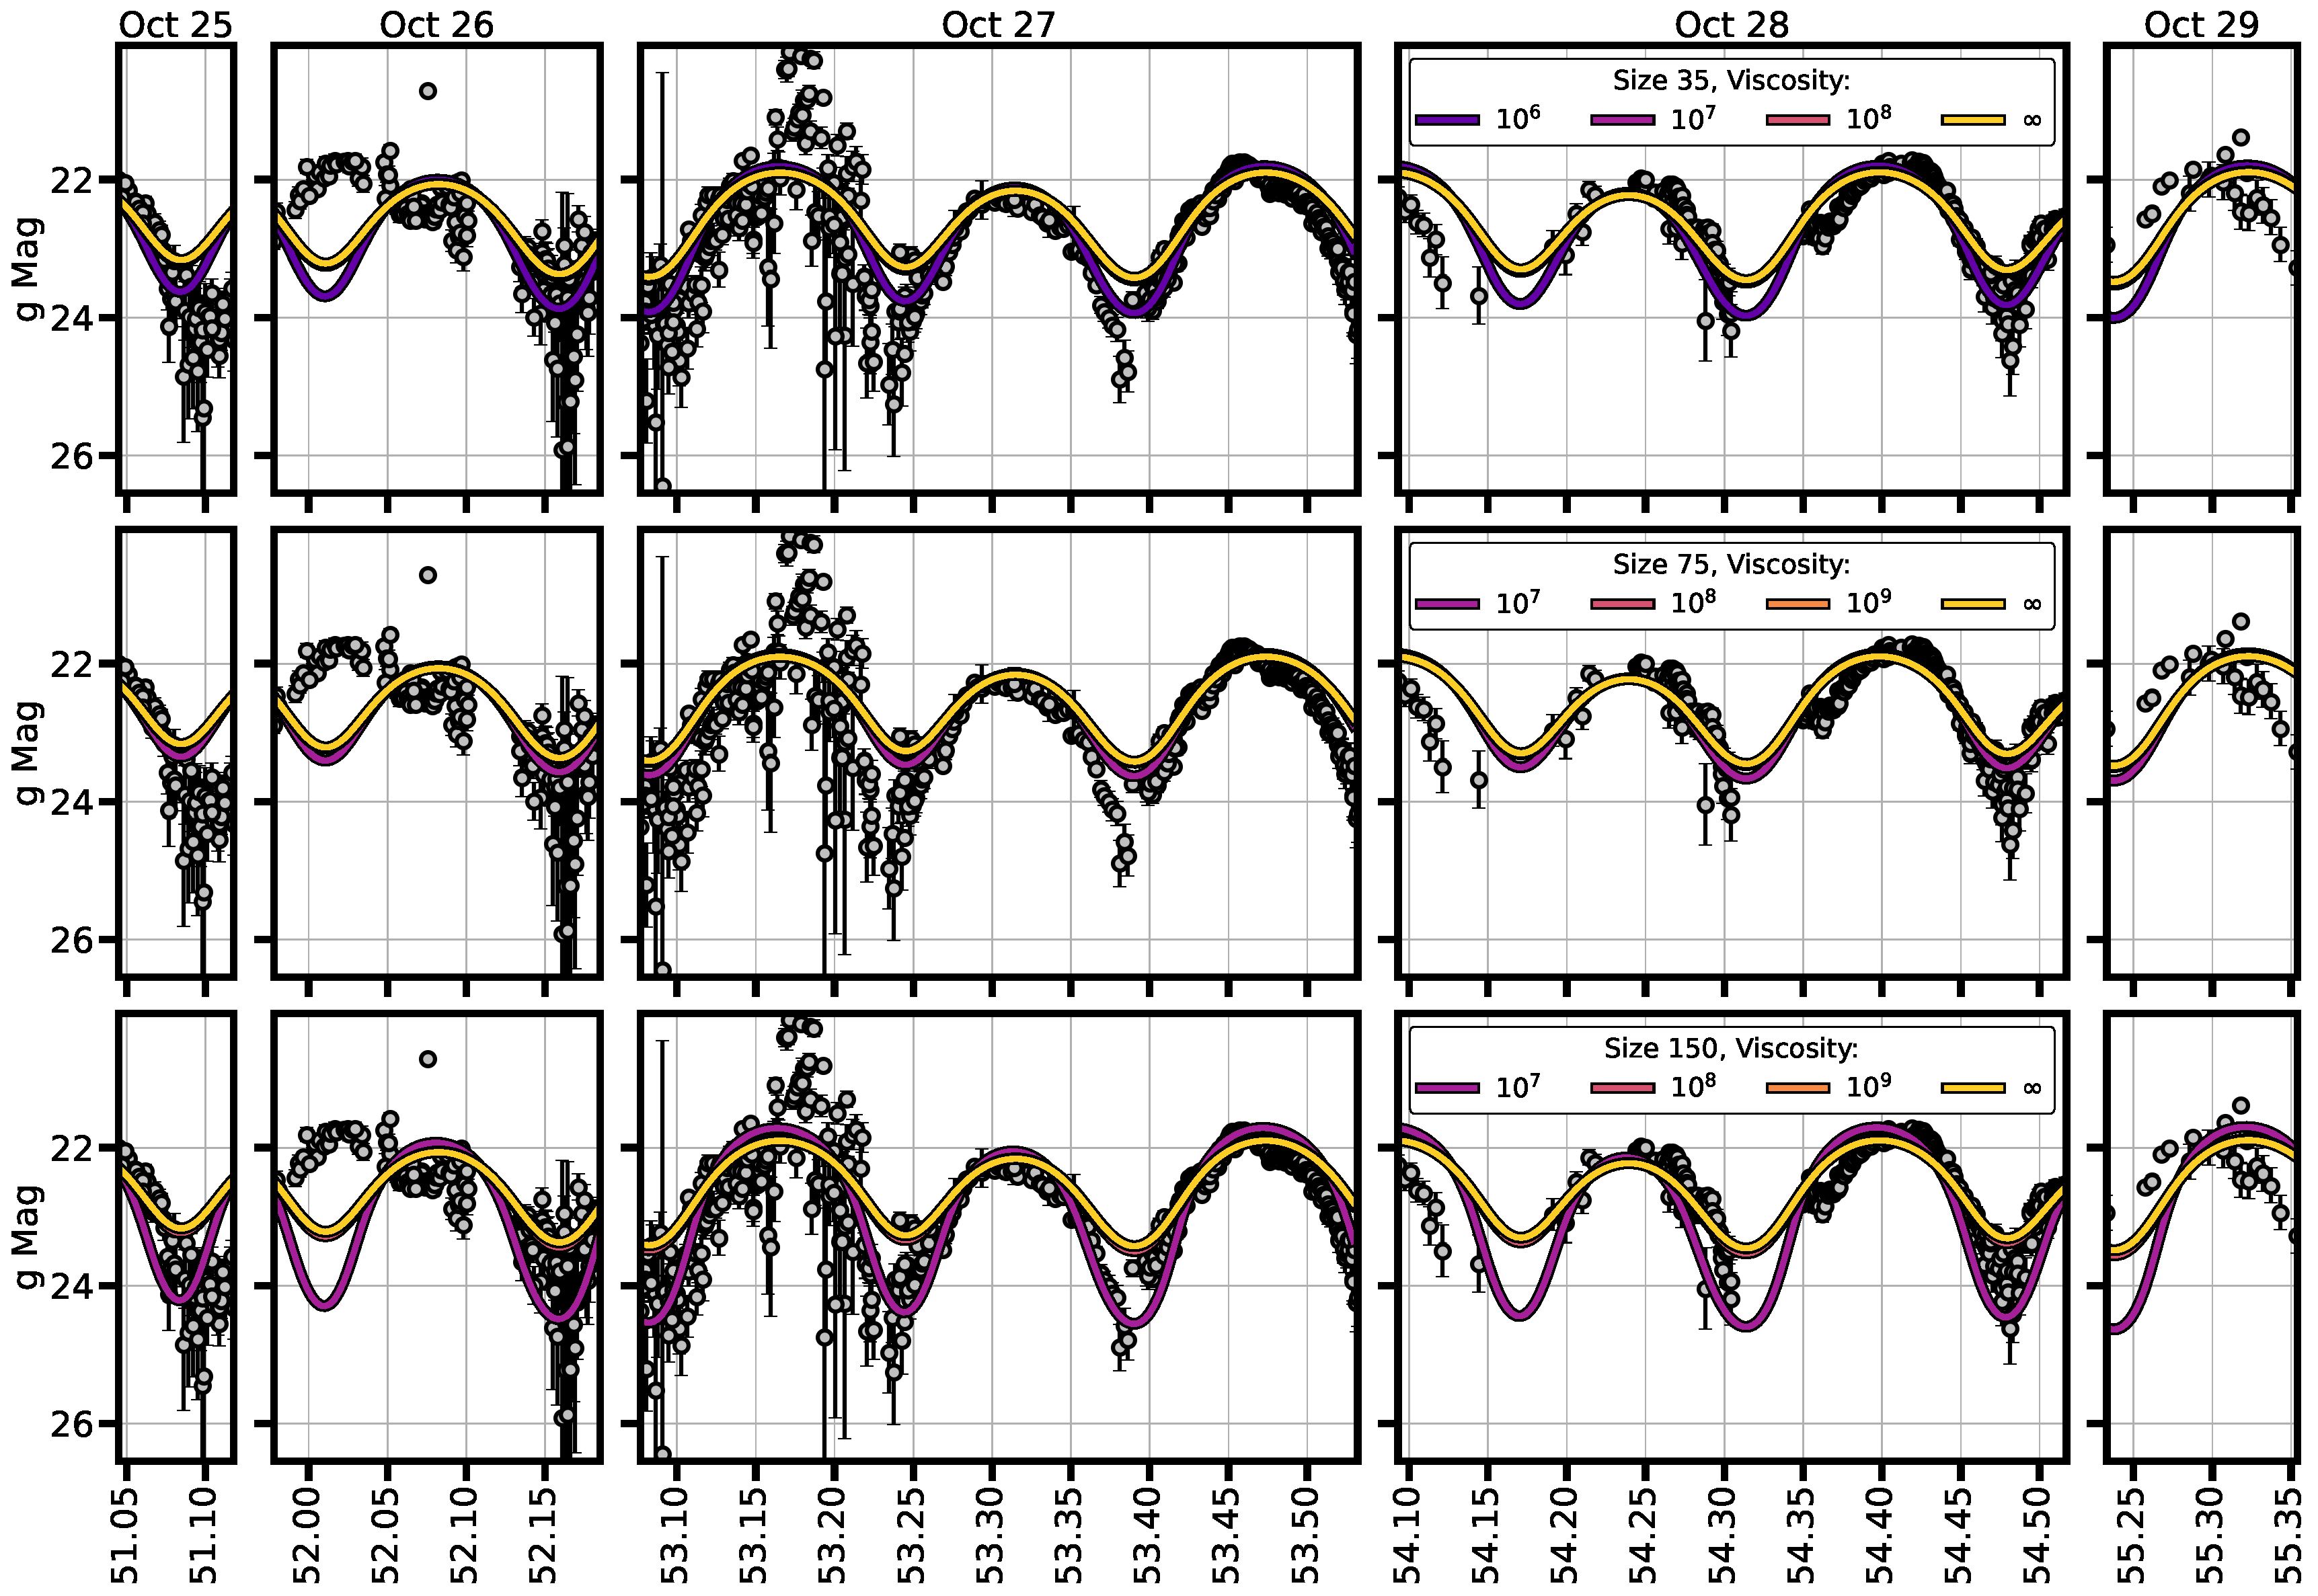
\includegraphics[width=.94\textwidth,angle=0]{optimal_sims_lightcurve_comp.pdf}
\caption{Synthetic light curves for `Oumuamua which incorporate simulated aspect ratio changes and constant period. Colored lines indicate the dynamic viscosity and photometric data are shown in grey points. These fits use optimized values of $\beta_0$ and $\Delta V$.}
\label{fig:optimalaxiscurvesimdata}
\end{figure*}

We also compare the synthetic light curves with the photometric data, assuming the optimal period of $p=7.3975$ hours. As in \S \ref{sec:lightcurvefits}, we optimize the initial rotation state $\beta_0$ and constant $\Delta V$ with \texttt{scipy.optimize.curve\_fit}, although we keep the remaining parameters constant. It is important to note that the spin-up between October and November (\S\ref{sec:lightcurvefits}) could not have been caused by tidal deformation. Therefore, the November data is optimized independently, assuming $p_\text{Nov}=7.1910$. In order to evaluate the validity of each fit, the $\chi^2$ values for both months are added together, which we present for each simulation in Table \ref{table:simdatachi2} and Figure \ref{fig:simdatachi2heatmap}. The resulting synthetic light curves along with the photometric data are shown in Figure \ref{fig:optimalaxiscurvesimdata} for October nights. 

\begin{figure*}
\centering
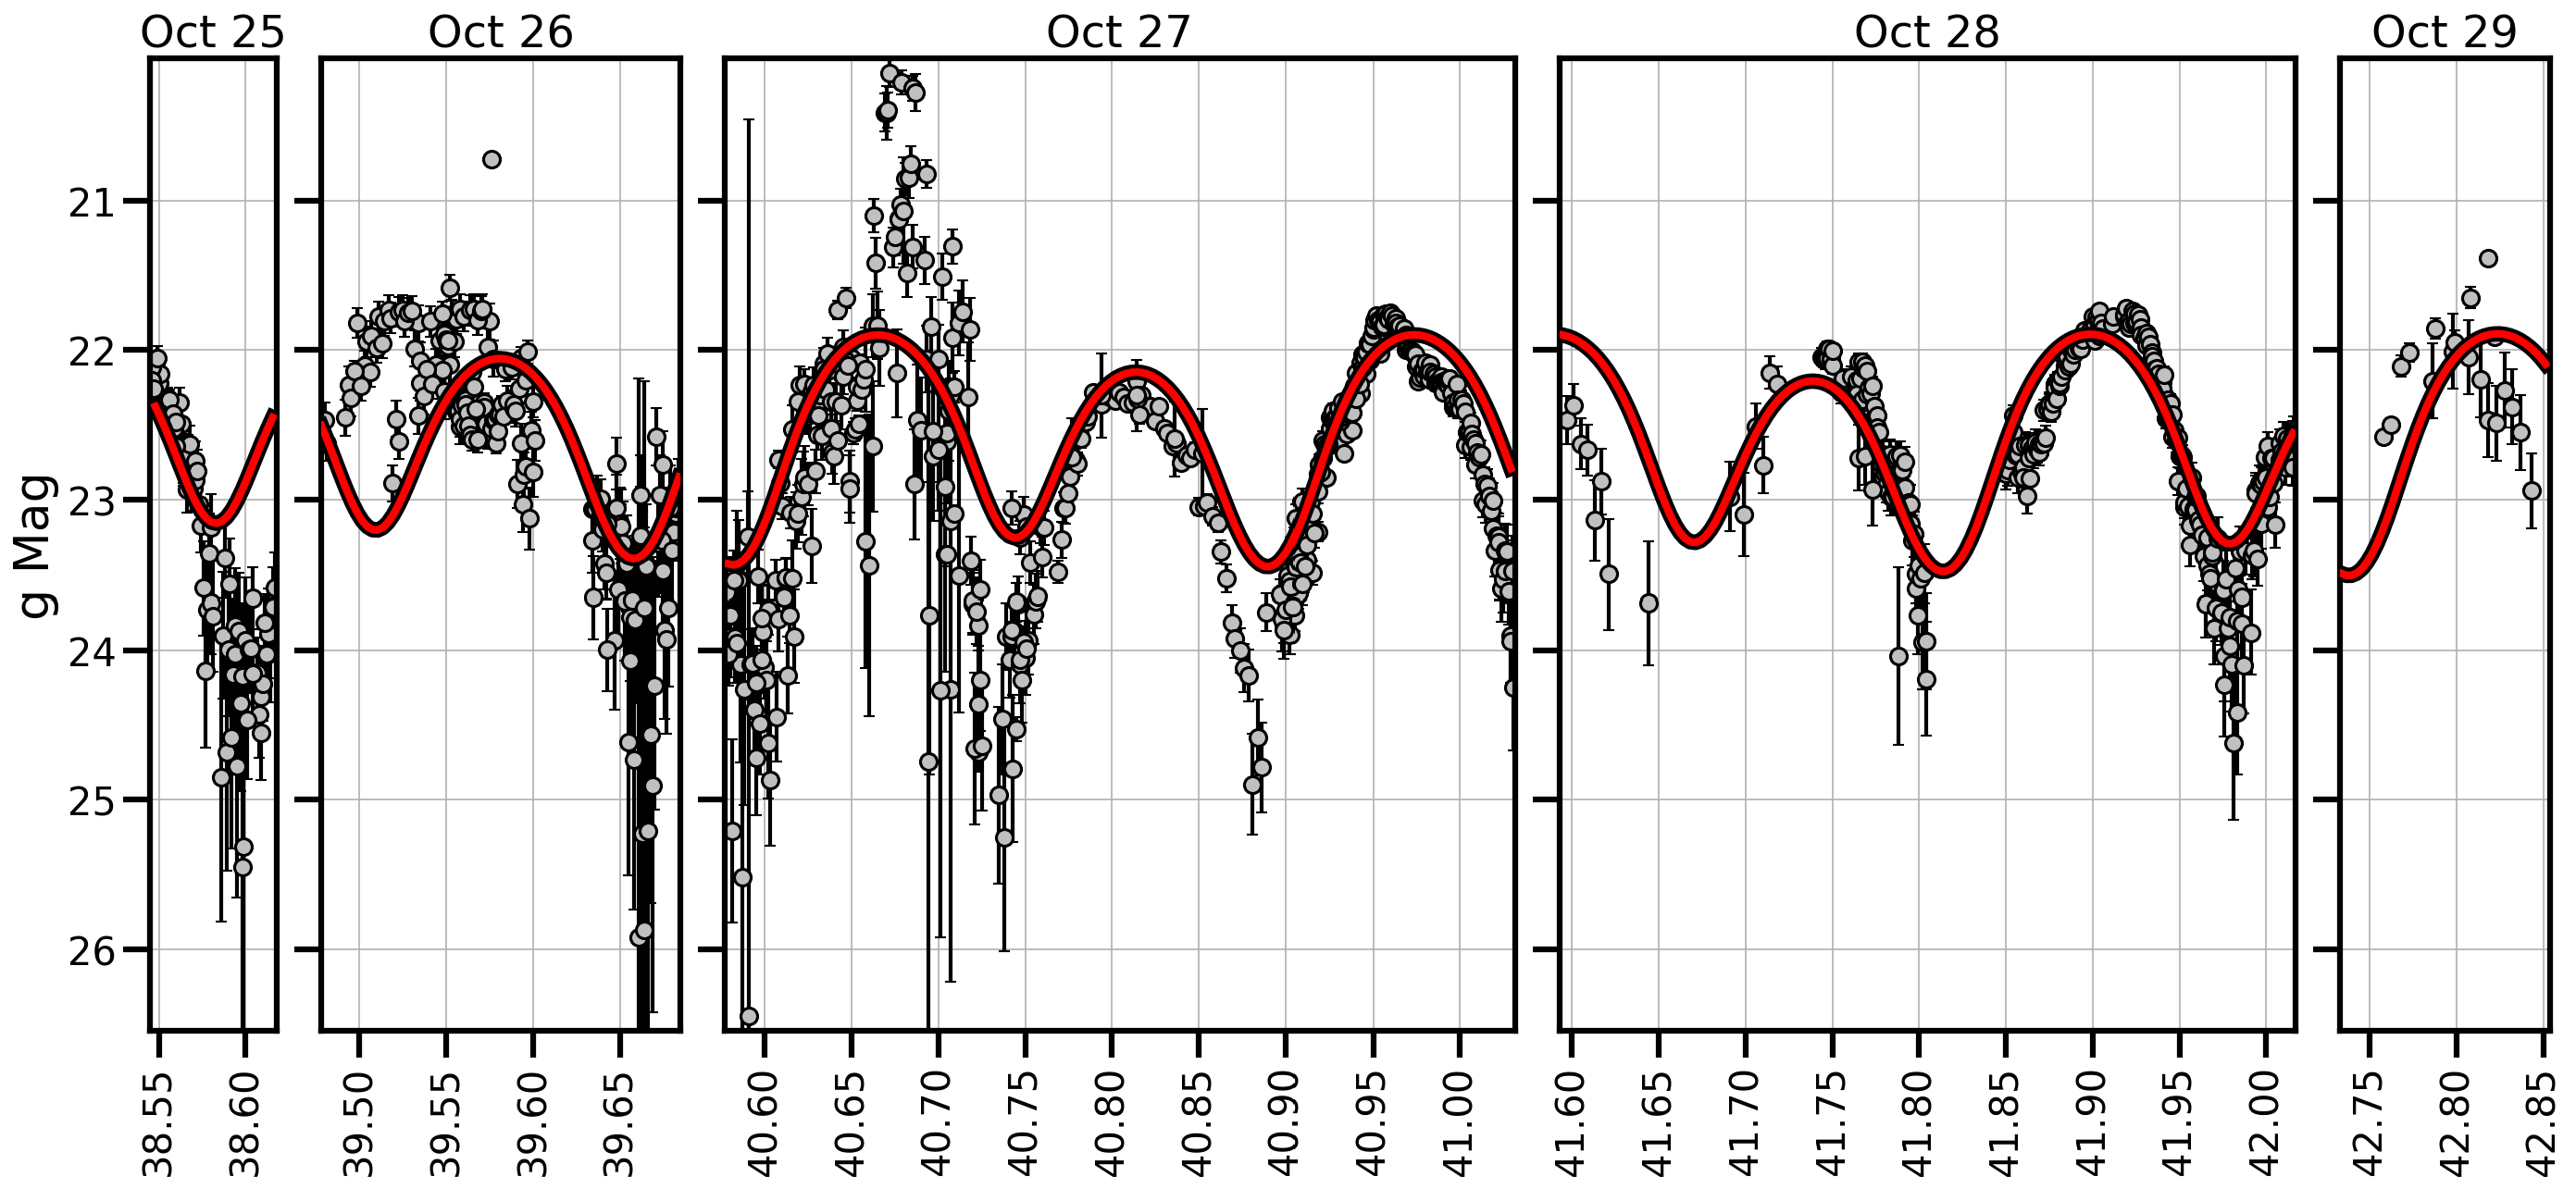
\includegraphics[width=\linewidth,angle=0]{optimal_sims_best_fit_lightcurve_comp.pdf}
\caption{The best-fit synthetic light curve (red line) and photometric data (grey points). This model incorporates the simulated changes in aspect ratio. Here $\mu=10^9$ g cm$^{-1}$ s$^{-1}$ and the body is initially 75 meters.}
\label{fig:optaxbestfitlightcurvesims}
\end{figure*}

A dynamic viscosity of $10^9$ g cm$^{-1}$ s$^{-1}$ and initial size of 75:75:12.5 meters produce optimal fits (discounting $\mu=\infty$), and this best-fit synthetic light curve is plotted along with the photometric data in Figure \ref{fig:optaxbestfitlightcurvesims}. It is worth noting that higher viscosity always produces a better fit for every initial size, therefore, no deformation provides the optimal explanation for `Oumuamua's light curve. 
 
\section{Discussion}\label{sec:discussion}
 
In this paper, we reported a spin-up in the photometric data of `Oumuamua between October and November. This change in spin period is distinct from and not in tension with the October spin-down reported by \citet{flekkoy2019}. We additionally argued that tidal deformation and outgassing could both contribute to the modulating periodicity in the observations. Although order-of-magnitude scaling analysis suggests that outgassing is the dominant contributing factor, we identify pathological cases where both forces are comparable. 

We further demonstrated that tidal deformation could produce observable spin-down for `Oumuamua. While our simulations show that deformation would not cause measurable amplitude variations for `Oumuamua, it is possible that this could be detected in other objects, depending on their bulk properties and albedo. It is feasible that the October spin-down was in part due to tidal deformation, while outgassing caused the spin-up between October and November. Dynamical simulations incorporating both of these effects would be worthwhile to perform in future work.

We presented simulations which incorporate tidal deformation of `Oumuamua, which we used to constrain its bulk viscosity and size. For the optimal 115:111:19 meter size found by \citet{mashchenko2019}, the dynamic viscosity must be $\mu\geq10^9$ g cm$^{-1}$ s$^{-1}$, roughly equivalent to the viscosity of bitumen pitch ($\mu\simeq 3\cdot10^9$ g cm$^{-1}$ s$^{-1}$) \citep{edgeworth1984}. Allowable dynamic viscosities are provided for different initial sizes in Table \ref{table:allowedviscosities}. `Stability' here describes cases with $<1\%$ change in the moment of inertia over the trajectory. These are extremely high viscosities --- for comparison, terrestrial fluids such as water or olive oil have viscosities of $\mu\simeq10^{-2}$ and $\mu\simeq1$ g cm$^{-1}$ s$^{-1}$, respectively \citep{crc2022,fellows2022}. However, the allowable viscosity range is compatible with a variety of terrestrial materials, including water ice ($\mu\simeq 10^{13}$ g cm$^{-1}$ s$^{-1}$) \citep{fowler1997} and the terrestrial mantle ($\mu\simeq 10^{22}$ g cm$^{-1}$ s$^{-1}$).

\begin{table}
\begin{tabular}{ |c|c| } 
 \hline
 \multicolumn{2}{||c||}{MINIMAL STABLE VISCOSITY} \\
 \hline\hline
 Primary Axis [m] & Viscosity [g cm$^{-1}$ s$^{-1}$] \\
 \hline\hline
 35 & $10^8$ \\
 \hline
 55 & $10^8$ \\
 \hline 
 75 & $10^9$ \\
 \hline
 115 & $10^9$ \\
 \hline
 150 & $10^9$ \\
 \hline
\end{tabular}
\caption{Stable dynamic viscosities for initial sizes of `Oumuamua.}
\label{table:allowedviscosities}
\end{table}

The second-largest dynamic viscosity remains relatively stable in all cases, with small changes in moment of inertia slightly larger than the $<1\%$ simulation cutoff. These viscosities allow for changing period and amplitude, while preventing nonphysical divergence of the body. It should be noted, however, that the highly stable viscosity of $10^9$ g cm$^{-1}$ s$^{-1}$ is orders of magnitude lower than the $10^{13}$--g cm$^{-1}$ s$^{-1}$ viscosity of water ice. Therefore, this constraint provides little differentiation between various solid ices.

Despite the limited constraints provided for the bulk composition of `Oumuamua, analyses of tidal deformation with these simulations may be useful for other small bodies. For objects with high rotation rates and closer solar approaches (such as 3200 Phaethon or 1866 Sisyphus), tidal and centrifugal forces will have a larger effect. This may be detectable in photometric data, and would enable more strenuous constraints on the physical properties of those objects. 

We have demonstrated that for simulated deformation, an initial size of 75 meters and a dynamic viscosity of $10^9$ g cm$^{-1}$ s$^{-1}$ provides an optimal match to the photometric data. For simulations with no deformation, a primary axis of 95 meters produces an equally good fit. 

`Oumuamua left many unanswered questions as it exited the Solar System, and despite intense scrutiny, there is still no general consensus regarding the provenance of the object. The discovery implies a spatial number density of similar objects of order $n_{o}\sim1-2\times 10^{-1}\,$au$^{-3}$ \citep{Trilling2017,Laughlin2017,jewitt2017,moro2018,Zwart2018,Do2018,moro2019a}. Detection and characterization of future interstellar objects offer the most promising avenue for resolving these questions. 

The forthcoming Rubin Observatory Legacy Survey of Space and Time (LSST) \citep{jones2009lsst,Ivezic2019} will effectively detect such transient objects \citep{solontoi2011comet,Veres2017,veres2017b,Jones2018}. The survey should detect $\sim$1 `Oumuamua-like interstellar object every year \citep{Moro2009,Engelhardt2014,Cook2016,Trilling2017,Seligman2018,Hoover2022}. In addition, the forthcoming NEO Surveyor \citep{Mainzer2015} may also detect interstellar objects, and could offer information about outgassing sources via its infrared capabilities. Space based in-situ measurements of an interstellar object would provide valuable information regarding the composition and bulk properties \citep{Hein2017,Seligman2018,Meech2019whitepaper,Castillo-Rogez2019,jones2019,Hibberd2020,Donitz2021,Sanchez2021,Meech2021,Hibberd2022,Moore2021whitepaper,Moore2021}. Additionally, future observations of the amplitude variations (if any) of interstellar objects may be used to constrain their bulk viscosities even without direct compositional measurements, via the techniques developed in this paper.

 \section{Acknowledgements}
This research utilized the University of Chicago’s Research Computing Center for numerical calculations. We thank Adina Feinstein for useful conversations and suggestions.

\bibliography{main}{}
\bibliographystyle{aasjournal}

\appendix

\section{Validation of Light Curve Fitting}\label{sec:lightfitvalid}

In this appendix, we validate our implementation of \texttt{scipy.optimize.curve\_fit} to optimize the rotation axis. We generate random combinations of parameters $p$, $\theta$, $\phi$, $\psi$, $\beta_0$, and $\Delta V$ which are used to generate synthetic light curves with ML15 for a 1-day period. We add Gaussian random errors to the synthetic data, with standard deviations three times the mean of the errors in the photometric data. We also re-scaled the error by the log of the square root of the magnitude to imitate photon noise.

We fit the ML15 model to the randomized data using random initial conditions drawn from Gaussian distributions about the true values. These initial conditions are unrealistically close to the true values compared to what we can achieve when optimizing real data. However, the meta-optimization performed in \S\ref{subsec:gettingaxis} overcomes this drawback and produces high quality fits.

In Figure \ref{fig:light_valid}, we show the true and noise added data and the optimal fit for a randomly drawn parameter set. This fit is extremely high quality, and the true value, optimized value, and statistical difference of the parameters are given in Table \ref{table:lightvalid}. Testing a variety of random parameters provides similar results (not shown). 

\begin{figure}
  \centering
  \begin{minipage}[b]{0.45\textwidth}
    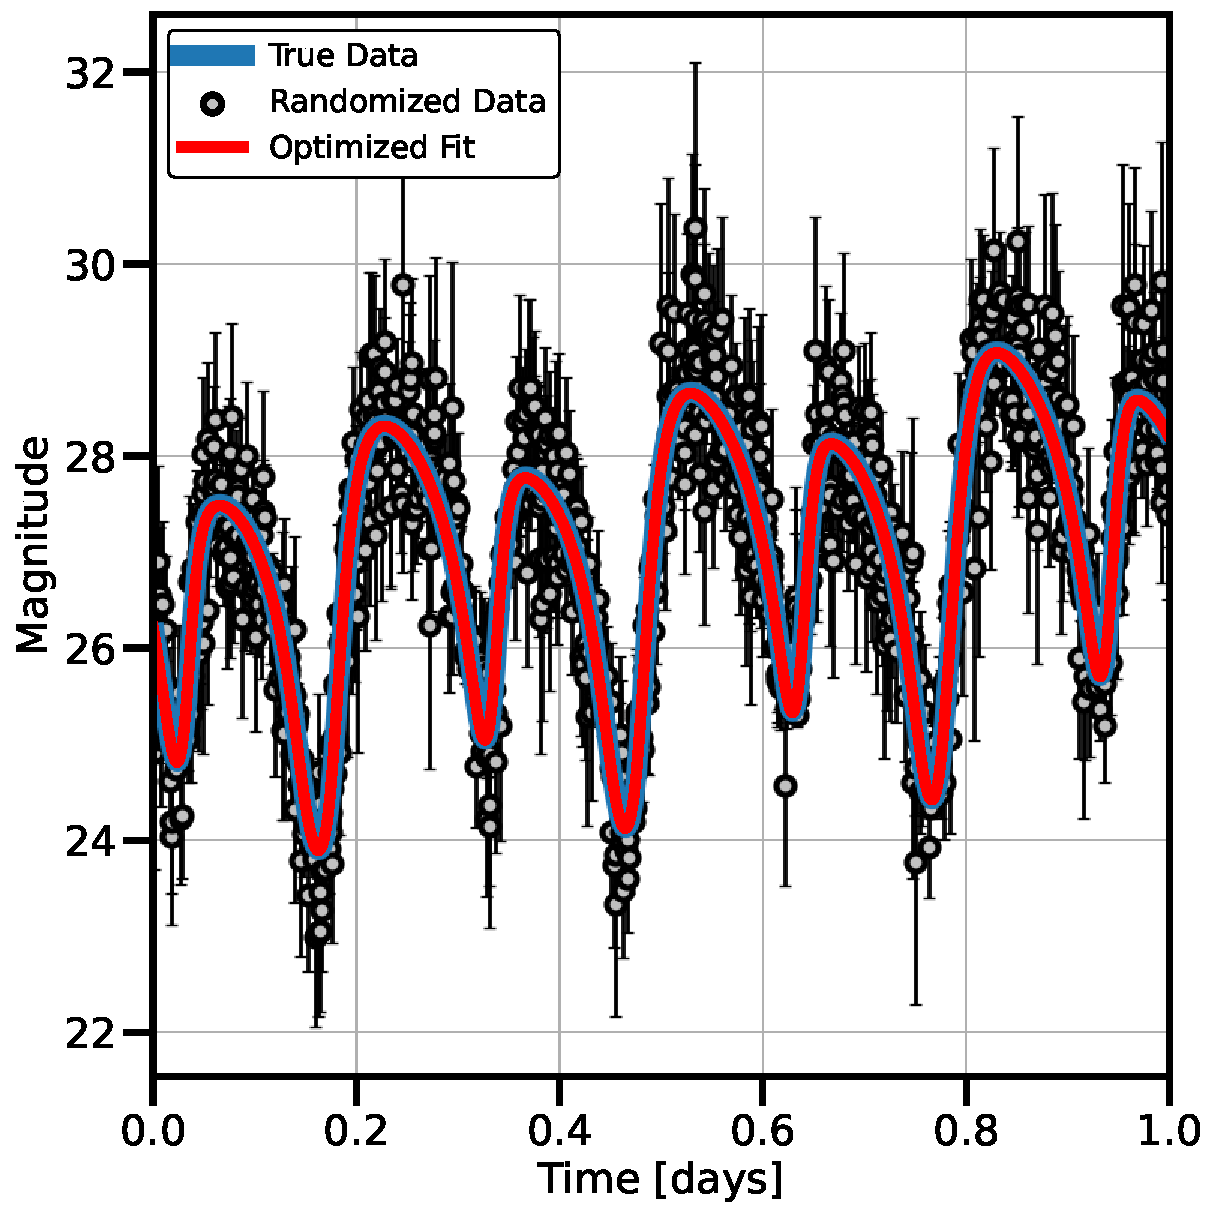
\includegraphics[width=\textwidth]{validation_lightcurve.pdf}
    \caption{Optimized fit (red line) for a random parameter choice. The true (blue line) and noise-added data (grey points) are also plotted for comparison. }
    \label{fig:light_valid}
  \end{minipage}
  \hfill
  \begin{minipage}[b]{0.45\textwidth}
    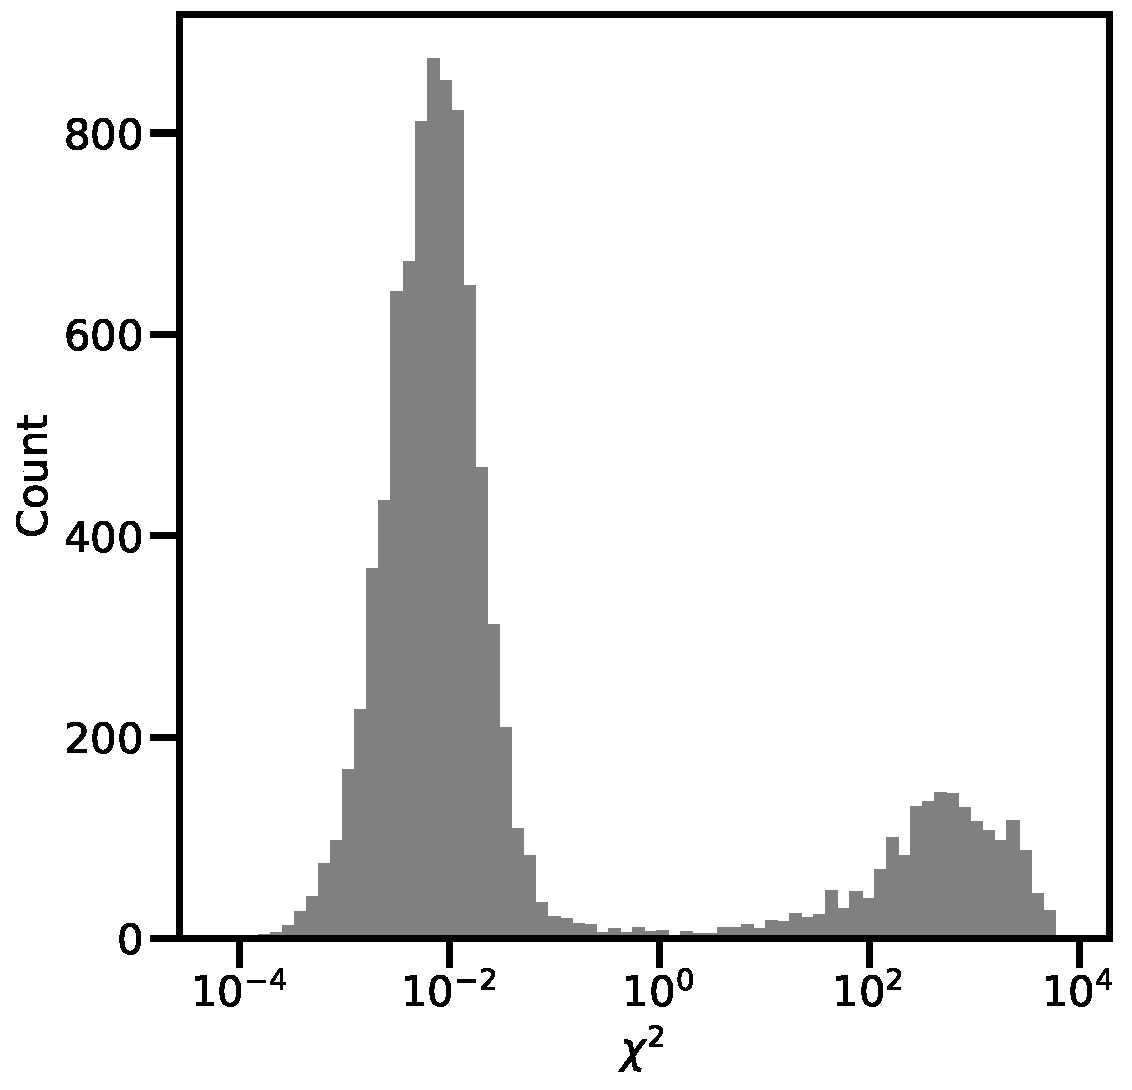
\includegraphics[width=\textwidth]{validation_chi2.pdf}
    \caption{The distribution of $\chi^2$ for $10^4$ synthetic light curves. The histogram marginalizes over all selected parameters, which were randomly chosen. }
    \label{fig:chi2_valid}
  \end{minipage}
\end{figure}

\begin{table}
\centering
\begin{tabular}{|c|c|c|c|}
 \hline
 \multicolumn{4}{||c||}{Parameters} \\ \hline\hline
 Parameter & True Value & Fit Value & Stat. Diff. \\ \hline
 $p$ & 7.2952 & 7.2954 & 0.414 \\ \hline
 $\theta$ & 5.7832 & 5.7832 & 0.022 \\ \hline
 $\phi$ & 0.5935 & 0.5916 & 1.418 \\ \hline
 $\psi$ & 0.2803 & 0.2797 & 1.043 \\ \hline
 $\beta_0$ & 0.3523 & 0.3522 & 0.252 \\ \hline
 $\Delta V$ & 33.3230 & 33.3265 & 1.402 \\ \hline
\end{tabular}
\caption{True and derived parameters for the synthetic light curve shown in Figure \ref{fig:light_valid}.}
\label{table:lightvalid}
\end{table}

We also perform this test for $10^4$ randomly sampled values, and plot their accuracy versus the estimated values in Figure \ref{fig:chi2_valid}. The majority of fits to synthetic data are very high-quality with $\chi^2\simeq10^{-2}$. Importantly, we verified that the distribution of $\chi^2$ shown in this figure is independent of the value of the randomized parameters and of the parameter itself (not shown for the sake of brevity). Clusters close to $\chi^2\simeq10^{-2}$ are nearly perfect fits, similar to those presented in Figure \ref{fig:light_valid}. This indicates that this optimization method is effective for any underlying set of parameters. 

\section{Dumbbell Model Validation}\label{sec:dumbval}

In this appendix, we validate the `dumbbell' model to represent the permanent quadrupole moment of `Oumuamua. We compare the behavior of Equation \ref{eq:tidal} with numerical integrations of tidal torques over a continuous body. 

The continuum force per unit volume is given by 
\begin{equation}
    \boldsymbol{F}_{\text{tidal}}=- GM_{\Sun}\rho\left(\frac{1}{(r_H-x)^2}-\frac{1}{r_H^2}\right) \,\big(\,\boldsymbol{R}*\boldsymbol{\hat{x}}\,\big)\,,
\end{equation}
where `*' indicates matrix multiplication. The torque is then $\boldsymbol{\tau}=\boldsymbol{d}\times\boldsymbol{F}$, where the distance from the rotation axis $\boldsymbol{d}$ is given by
\begin{equation}
    \boldsymbol{d}=\boldsymbol{r}-(\boldsymbol{r}\cdot\boldsymbol{\hat{\Omega}})\boldsymbol{\hat{\Omega}}\,
\end{equation}
for a position vector $\boldsymbol{r}$. 

The torque on `Oumuamua is evaluated with Equation \ref{eq:tidal} on a $100\times500$ grid for $\beta\in[0,\pi)$ and $r_H\in[0.257,3.147]$ au, with $\boldsymbol{\hat{\Omega}}=(0,1,0)$. Numerical integrals are computed over the same grid with the \texttt{quadpy} package \citep{quadpy}. The integral domain is the set of $(u',v',w')$ Cartesian points in the unit 3-ball $\mathcal{S}$, transformed via
\begin{equation}
    \begin{dcases}
        x'=\frac{a}{2}u'\\
        y'=\frac{b}{2}v'\\
        z'=\frac{c}{2}w'\,.
    \end{dcases}
\end{equation}
These relationships define an isomorphic mapping $(x',y',z')\rightarrow(u',v',w')$ from $\mathds{R}^3\rightarrow\mathds{R}^3$. The determinant of the Jacobian is $du'dv'dw'=8abc\,dx'dy'dz'$, which finalizes the transformation. We again define the fractional error as $E_{\rm frac}=|(\text{ana}-\text{num})/\text{ana}|$ for numerical (num) and analytic (ana) values, and show this in Figure \ref{fig:valid_ratio_curve}. We verified that the error had no dependence on $r_H$.

\begin{figure}
\centering
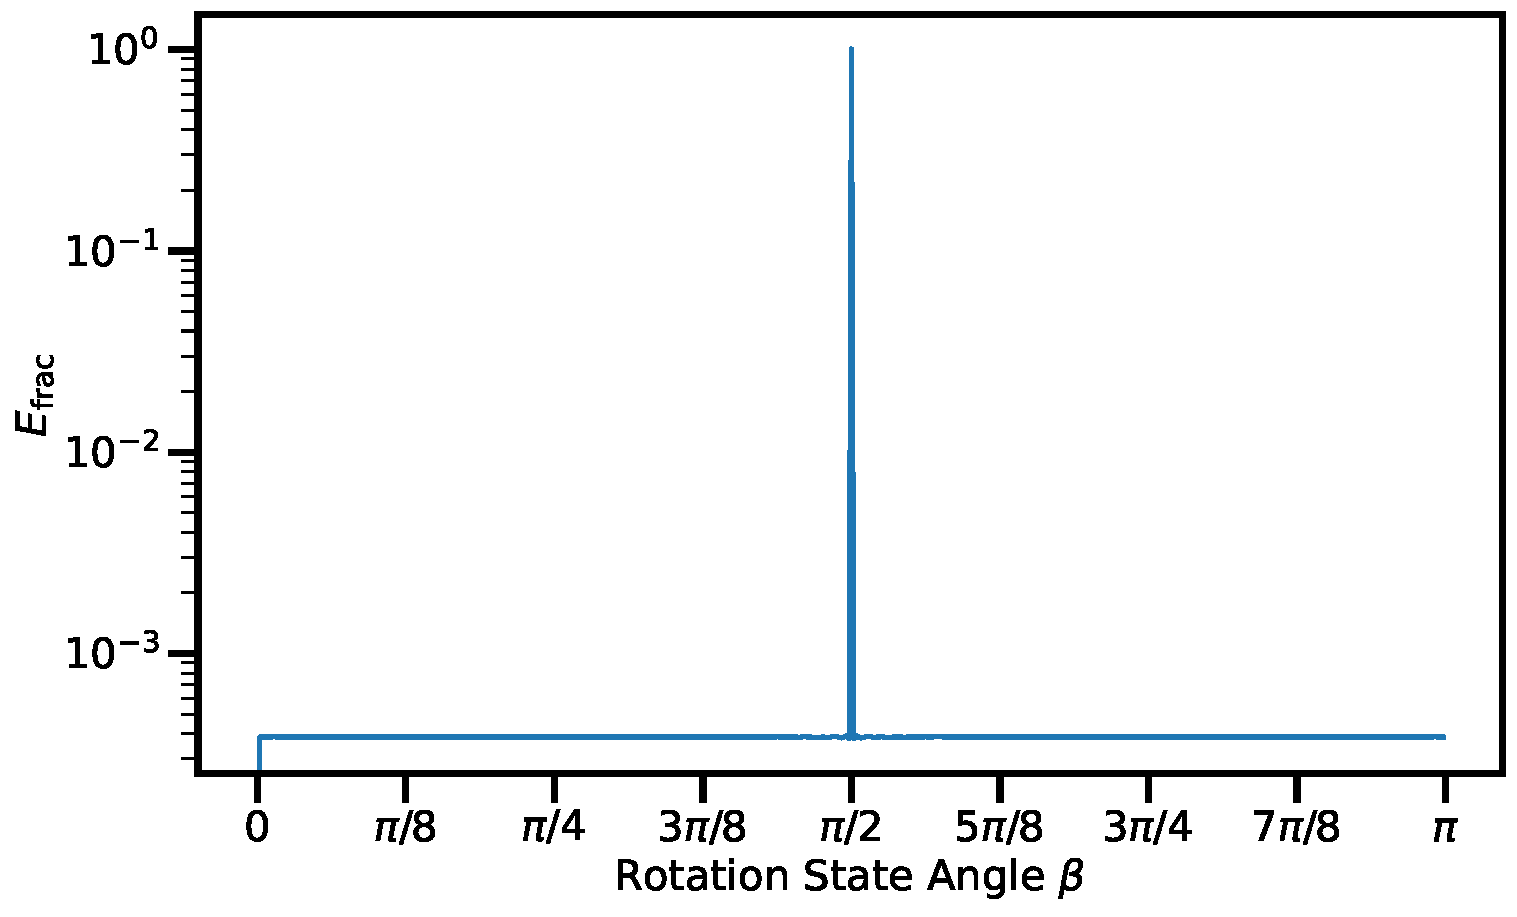
\includegraphics[width=.5\textwidth,angle=0]{validation_ratio_curve.pdf}
\caption{Fractional error of the `dumbbell' model compared to numerical integrations of the total torque at fixed $r_H=1$ au.}
\label{fig:valid_ratio_curve}
\end{figure}

The central spike where $E_{frac}\simeq1$ at $\beta=\pi/2$ in Figure \ref{fig:valid_ratio_curve} corresponds to where the numerical solution is significantly smaller than the analytical solution. The maximum value of the analytic and numerical torques are $\mathcal{O}(10^{-8})$, and $\mathcal{O}(10^{-10})$ respectively. The true value of torque is exactly 0 here due to symmetry, and while both methods are close to the true value, the comparison fails due to rounding errors. Besides this pathological orientation, the `dumbbell' model accurately depicts the torque on an ellipsoidal body with errors $\mathcal{O}(10^{-4})$.

\section{Cigar-shape Tidal Torque}\label{sec:cigtor}

In this appendix, we demonstrate that the tidal torque is equal for a ``cigar"- and ``pancake"-shaped body (\S\ref{sec:tidana}). We assume now that $b=c$, $a>c$. Setting Equations \ref{eq:dumbbellquad} and \ref{eq:ellipsoidquad} equal, the points are at $(\pm R,0,0)$, with $R\equiv\sqrt{a^2-c^2}$ and mass given by $m=(4\pi/15)abc\rho$. We again assume rotation about the y-axis, so when the point masses are rotated about the x-axis by an angle $\beta$, the masses are at $\pm (R\cos\beta,0,-R\sin\beta)$. The acceleration on the center of mass is given by Equation \ref{eq:comacc}, and the acceleration on each of the points is equal to Equation \ref{eq:torqueforce}. The tidal acceleration is the difference in these accelerations, the force is given by Equation \ref{eq:torqueforce}, and the lever arm is $\pm (R\cos(\beta),0,-R\sin(\beta))$ for $m_1$ and $m_2$ respectively. Therefore, the resulting tidal torque is 
\begin{equation} 
\begin{aligned}
\begin{dcases}
    \boldsymbol{\tau}(m_1)=- G M_{\Sun} m \left( \frac{1}{(r_H-R\cos\beta)^2}-\frac{1}{r_H^2} \right) [(1,0,0)\times+(R\cos\beta,0,-R\sin\beta)]\\
    \boldsymbol{\tau}(m_2)=- G M_{\Sun} m \left( \frac{1}{(r_H+ R\cos\beta)^2}-\frac{1}{r_H^2} \right) [(1,0,0)\times-(R\cos\beta,0,-R\sin\beta) ].
\end{dcases}
\end{aligned}
\end{equation} 
The vector component is $\mp R\sin\beta\,\boldsymbol{\hat{y}}$. Simplifying using $m=(4\pi/15)abc\rho$, $R=\sqrt{a^2-c^2}$, $b=c$, and $\epsilon=c/a$, the magnitude of the total torque along the rotation axis ($\boldsymbol{\hat{y}}$) is
\begin{equation}
    \tau=(\frac{8\pi}{15}GM_{\Sun})\left(\frac{r_Ha^5\rho\epsilon^2(1-\epsilon^2)\sin{(2\beta)}}{(r_H^2-a^2(1-\epsilon^2)\cos^2(\beta))^2}\right ).
\end{equation}
Note that apart from an $\epsilon^2$ to account for the different sizes of $b$, this is equivalent to Equation \ref{eq:tidal}.

\end{document}
